% Template for ICIP-2013 paper; to be used with:
%          spconf.sty  - ICASSP/ICIP LaTeX style file, and
%          IEEEbib.bst - IEEE bibliography style file.
% --------------------------------------------------------------------------
\documentclass[a4paper]{article}
\usepackage{spconf,amsmath,graphicx}
%\usepackage{epsfig}
\usepackage{amssymb}
\usepackage{subfigure}
\usepackage{cite}
\usepackage{multirow}
%\usepackage{epstopdf}
\usepackage{amsmath}
\usepackage{geometry}
\usepackage{tikz}
\usepackage{color, soul}
\usepackage[style=base]{caption}
\usepackage{lineno}
\usepackage{comment}
\usepackage{array}  
\usepackage{siunitx}
\usepackage{mathtools}
\usepackage{bm}
\usepackage[version=4]{mhchem}
\usepackage{cite}
\usepackage{amsmath,amssymb,amsfonts}
\usepackage{algorithmic}
\usepackage{graphicx}
\usepackage{textcomp}
\usepackage[ruled, lined, linesnumbered, commentsnumbered, longend]{algorithm2e}
\usepackage{xcolor}
\usepackage{epsfig}
\usepackage[numbers]{natbib}
\usepackage[final]{pdfpages}
\usepackage{multicol}
\usepackage{listings}

\usepackage{hyperref}
%\usepackage[noabbrev]{cleveref} % If you want "figure X" instead of "fig. X"
\usepackage{cleveref}
\usepackage{csquotes}

\begin{document}
\onecolumn
\includepdf[pages=-]{front_page.pdf}

\section*{Foreword}

Denne oppgaven tok ikke 3 måneder å skrive, det tok 5 år med arbeid, læring, møter med fantastiske mennesker, egen læring, og dedikasjon.

Jeg vil ønsker å takke alle mine venner som har støttet meg under skrivingen, og trøstet meg i de tunge tidene. En stor takk til Mahrin Tasfe, Emma Sofie Rikheim \& Celine Hagen, Vegard Eriksen Sæther, Bee, og Sindre Stokke for å passe på at jeg ikke overarbeidet meg, og kunne få en puste pause under denne intense perioden.

jeg vil også strekke ut en takk til Spillforeningen Både Kort og Bredt, og Rollespill gruppen som jeg deltar i for å gi meg noen morsomme øyeblikk og noe å glede meg til når oppgaven er levert inn.

Jeg ønsker også å gi en stor takk til Studentlivssenteret i Ås og Ås Helsestasjon for den hjelpen og de tilbudene de gir til studentene og som jeg fikk bruke. Mental helse er helse og det viste seg under skrivingen, og er evig taknemelig for gratis tilbudene de tilbyr.

Jeg vil også takke veilederne mine; Mareile Wolff, Berit Nordskog, og Brita Linnstad for å ta meg imot og være tolmodig med meg mens jeg fant ut av ting underveis dette semesteret. Dere har vært flinke veiledere.



\section*{Abstract}
This study focuses on 3 models that have been used in the literature to predict soil temperatures. The depths chosen as targets are 10cm, and 20cm in 4 regions; Innlandet, Østfold, Vestfold, and Trøndelag. In each region there are 4 stations spread along the region to get the most coverage of area to be the most representative of the local area. The models chosen had been used in the literature to predict soil temperatures. The data used in this study was collected from \acrshort{ac:kilden} with the features; hourly air temperature from 2m height, soil temperature from 10cm depth, soil temperature from 20cm depth.

The models chosen are LSTM, BiLSTM, GRU, linear regression, and linear regression model modified by \citeauthor{plauborg_simple_2002}. All the models performed within 2$^\circ C$ RMSE and an absolute bias of 1.5|$^\circ C$| except linear regression that had an RMSE of 4.5℃ RMSE  and absolute bias of 

\section*{Oppsumering}
Denne studien ser på modeler som predikerer jordtemperaturer

% hva gjør vi

% metode

% resultat

%Er det kun økonomiske og tekniske årsaker til at vi ikke måler overalt? Det er mange steder hvor det ikke er mulig å måle. Det er heller ikke mulig å ha et uendelig antall sensorer over alt. Det finnes mange steder hvor en ønsker å beregne jordtemperatur hvor det er en viss avstand til en eksisterende værstasjon, kanskje det er andre geografiske forhold, eller lokale klimaforhold som påvirker. Som du skriver, er det også ønskelig å kunne beregne jordtemperatur fremover i tid.

\keywords{LSTM, GRU, RNN, Soil temperature, Machine learning, regression,hourly, weather forecasting data}

\section{Introduction}

In agriculture soil temperature is one of the important parameters to put into consideration when thinking about pest prevention, conservation, and yield prediction. The reasoning for this is that knowing the soil temperature is gaining useful insight into
gain important info for water management \cite{alizamir_advanced_2020},
potential yields \cite{sim_prediction_2020},
calculation of plant-growth \cite{li_modeling_2020},
and predicting hatching insect eggs\cite{nanushi_pest_2022,johnson_effects_2010}.
Being able to predict the soil temperature a few days in advance does give insight into
potential flooding and erosions\cite{stuurop_influence_2022},
when seeds start to sprout \cite{li_modeling_2020},
nitrogen processes \cite{rankinen_simple_2004} in the soil.
Due to climate change it is more important to know soil temperatures at given depths.

If it's important, why don't institutions measure it everywhere? There are several reasons for this, but a common reason is that it's expensive to install new equipment on old weather stations. Furthermore, it is unfeasible to install sensors absolutely everywhere at any depth, however it is not necessary with full coverage of an area as it is sufficient to have a few samples here and there to get an overview of the current state of the soil. Another thing is that it might be impractical to install sensors in some areas due to climate, soil quality (or lack there of), or the misrepresentation of the area if it's a geographical or meteorological special case.

Sometimes the weather station do have the sensors in the fields reading soil temperature at given levels, but due to technical misadventures and unforeseen phenomenons there might be gaps or misreadings that need to be replaced with approximations or NULL values\footnote{These values are different from 0 as they represent "no data" and can't be used to do calculations.}.

Previous research has investigated soil heat conductivity, leading to the formulation of differential equations \cite{karvonen_model_1988}. However, these mathematical statements, which involve heat transfer, are computationally demanding and challenging to simulate or calculate \cite{fourier_analytical_2009, karvonen_model_1988}. Numerical solutions are not the only obstacle; the dynamic nature of heat within the soil also plays a crucial role. For instance, frost in Scandinavian countries significantly alters soil heat conductivity \cite{stuurop_influence_2022}, further complicating accurate calculations. As part of this study, data will be collected from Norway, situated within the Scandinavian region.

Deeplearning models

A beneficial model would be one using the fewest number of parameters as possible while returning results within acceptable tolerances. This study will consider models that can use only time and air temperature as those two features are the most common measurements measured at weather stations, since soil temperature is not necessarily calculated as stated earlier. A good metric in this study will be considered to be a combination of Root Mean Square Error and Explained Variance (see section \ref{sec:method:metric}). 

This study aims to address the following key questions:
\begin{itemize}
	\item Achieving Good Results with Minimal Parameters: Can satisfactory predictions be obtained using a limited set of meteorological and chronological parameters?
	
	\item Deep Learning Models for Soil Temperature Prediction: Is it feasible to employ deep learning models for predicting soil temperatures?
	
	\item Complexity of Deep Learning Models: Is it necessary to utilize complex deep learning architectures when predicting soil temperatures?
	
	\item Suitable model for Nordic climate: Is there a model that fits for the Scandinavian climate?
\end{itemize}

Regarding deep learning models, this study primarily focuses on \gls{gl:rnn} networks and explores various compositions of this technology. The definition of a "good result" will be relative to the performance of other models in the field and to similar studies that employ comparable architectures. Additionally, the \acrfull{ac:gru} has been considered as an alternative to LSTM in this context due to its simplicity, and yet mechanically similar to the LSTM.


\section{Theory}\label{sec:theory}

This section discusses the theory behind the models used in the study, with the first section being general information about the soil and use cases of soil temperature in agriculture.

\subsection{Soil temperature}

The difficult in predicting the soil temperature comes from that the environment is highly variant and radically different from each other. A farmer in Sunndal in Middle-Norway would have to do different considerations than a farmer in Bergen in Sør-Norge simple due to different climate and soil profile. There exist methods to help farmers get an local estimate of current soil state, one of which are using a soil thermometer. These methods works to make on-the-spot decision to when plant crops, water the crops, or when to harvest. A better approach is to have a model to predict the upcoming temperatures so farmers have a window of time to prepare for crop harvest or planting.

An application of the soil temperature is used as a mean of agricultural advise is the study conducted by \acrshort{ac:nibio} where they look at the mean five-day air temperature compaired to the mean five-day soil temperature to asses when it is useful to start sowing the seeds\cite{nordskog_jordtemperatur_2018}. 

A way to measure soil temperature is to insert a rod into the ground and measure, however to measure multiple depths there are usually three ways to do it; one rod to measure all the depths, one rod for each depth, and a hybrid solution of the first and the second method. There are two sensors that are being used
\begin{enumerate}
	\item Model 107 Temperature Probe\cite{noauthor_107_nodate}
	\begin{itemize}
		\item Tolerance: $\pm0.2^\circ C$ (over the $0^\circ C$ to $50^\circ C$ range)
		\item Measuring Range: $-50^\circ C$ to $+100^\circ C$
		\item Probe Diameter: 0.76 cm (0.3 in.)
	\end{itemize}
	\item PT500 temperature sensor\cite{kamstrup_dokumentasjon_nodate}
	\begin{itemize}
		\item Measuring Range: They have a broad measuring range, usually from $-50^\circ C$ to $+400^\circ C$
		\item Long-term Stability: PT500 sensors are known for their high long-term stability, making them reliable for continuous use over long periods.
		\item Construction: These sensors are constructed with platinum, which contributes to their precise measurements and robustness.
	\end{itemize}
\end{enumerate}

There are a few depths to choose to monitor, on of those ranges are 5 cm to 15 cm range that is the root zone\cite{jones_sb_35_nodate}. The root zone is an range where the roots of plants where the highest density of roots are, and at the end of the root zone researchers can gather information about droughts and snow-melts that are filling up og depleting the root system. 

A simple naive way to predict soil temperature would be to use the equation found by \cite{van_wijk_wr_periodic_1963}
\begin{equation}
	\text{daily soil temperature} \approx \widetilde{T}_{\text{soil,year}} + e^{-z/D}\sin(\omega t - z/D + \phi)
\end{equation}

This analytical formula has its limitations as it does not take into account rain fall, snow melt, freezing, and re-freezing. Further more, the formula does not incorporate the importance of the surface temperature and its inpact on the soil layers over time. An ideal formula would incorporate all of these elements and possibly more, but that would require more computation power than currently available.

An expantion of this soultion was expanded by \cite{roodenburg_estimating_1985} by including the solar movement to predict daily soil temperatures. The sun does heat up the soil differently depending on it angle over horizon and the cloud blocking or not hiding the sun. It is commented by the author of \cite{roodenburg_estimating_1985} that this simple model does not describe the soil temperature the effect of snow cover or precipitations effects.

From current understanding of soil physics a modern model researches in cooperate the saturated hydraulic conductivity and the unfrozen water content to their equations\cite{stuurop_influence_2022}. Some of these formulas contains nested exponentials\cite{stuurop_influence_2022}. This formulation introduces numerical limitations as the estimation at the center of the formula would be amplified as the computation continues. A commonly used approch is \acrfull{ac:fdm} where a differential equation gets decomposed to several equation that gets mapped to a grid with boundary conditions\cite{singh_numerical_2017,rankinen_simple_2004,cleall_analytical_2015}. 

\subsection{Linear Regression}\label{sec:theory:linreg}

Air temperature has a direct connection to soil temperature as the main source of thermal energy next to solar radiation. This study chose this model for its simplicity and being the simplest model to be considered. A primitive relation between air temperature and soil temperature at a given depth would be the equation \eqref{eq:linmod}.

\begin{equation}
	T_{\text{Soil, n cm}} \approx \beta_{\text{n cm}} T_{\text{Air}} + \vec{\varepsilon}\label{eq:linmod}
\end{equation}
The $\beta_{\text{n cm}}$ represent the scaling factor for the air-soil relation. The regression model will be for the sake of convenience be expressed as the following expression
\begin{equation}
	\vec{F}(\mathbf{A})\vec{\beta}=\vec{y}+\vec{\varepsilon}.
\end{equation}

Where $\vec{F}$ is a vector function with following domain $\vec{F}:\mathbb{R}^{n\times m}\to \mathbb{R}^{n\times p}$ where $m,n,p\in \mathbb{N}$, $\mathbf{A}$ is the data in matrix form with dimensions $\mathbb{R}^{n\times m}$, $\vec{\beta}$ is the regression terms with shape $\mathbb{R}^{p\times 1}$, $\vec{y}$ is the target (TJM10 or TJM20) with shape $\mathbb{R}^{n\times 1}$, and $\vec{\varepsilon}$ is the residual error with the same shape as$\vec{y}$.

This will function as the base model to compare to the plauborg model in section \ref{sec:theory:pluborg}.

\subsection[Plauborg Regression]{Plauborg Linear Regression model with Fourier terms}\label{sec:theory:pluborg}
The model developed by \cite{plauborg_simple_2002} was trained in Denmark hand has shown promising results for a Scandinavian model. For that reason it was included in this study 

An improvement over an time independent Linear Regression model would be a time dependent Linear Regression model that takes not only current time into account of the calculations but also previous measurements. It is current knowledge that soil temperatures depends on previous temperatures and meteorological phenomenons. In the paper \citeauthor{plauborg_simple_2002} \cite{plauborg_simple_2002} extend the features from only air temperature at current time to include also previous days of year and the air temperature from those days as an extension of \cite{roodenburg_estimating_1985}. This means the following F function that \citeauthor{plauborg_simple_2002} used would be 
$$
\vec{F} := [air_t , air_{t-1}, air_{t-2}, air_{t-3}, \sin(\omega t) , \cos(\omega t), \sin(2*\omega t), \cos(2*\omega t)]^T.
$$

Where $air_t$ is the air temperature at time $t$ expressed in day of the year (0-365), $\omega$ is the angular frequency in radians per hour or radians per day, depending on the time unit. The sine/cosine elements in the F function represent the variations through the day by fitting $\vec{\beta}$ to the yearly variation. To adapt the authors model to an hourly time unit would be to either
\begin{enumerate}
	\item Extend the F function to include a larger $\omega$ coefficient to reflect hourly oscillations in conjunction with daily fluctuation
	\item Refit the Fourier terms with a larger $\omega$ coefficient to make the oscillations more representative of daily temperature changes.
\end{enumerate}

The larger coefficient could be expressed as $2\pi/24$ while the smaller $\omega$ for daily values would be rescaled to $2\pi/365$.

The problem with this approach would be Fourier Sine-Cosine series approximation which would suggest that \citeauthor{plauborg_simple_2002}'s method could be subject to overfitting with addition of more terms on a small dataset. On the other hand it gives us a way to compute the coefficients $\alpha_i$ and $\gamma_i$ for sine and cosine terms respectively, though it would be more numerically stable with a pseudo-inverse computation or a max log likelihood approach. However, the python module used in this study utilizes a different algorithm described in this paper \cite{van_benthem_fast_2004} that performs an iterative method of solving $\underset{\beta}{\text{argmin}} \left|X\vec{\beta} - \vec{y}\right|$.

\subsection{\acrfull{ac:lstm} model}\label{sec:theory:lstm}

\begin{figure}[ht]
	\centering
	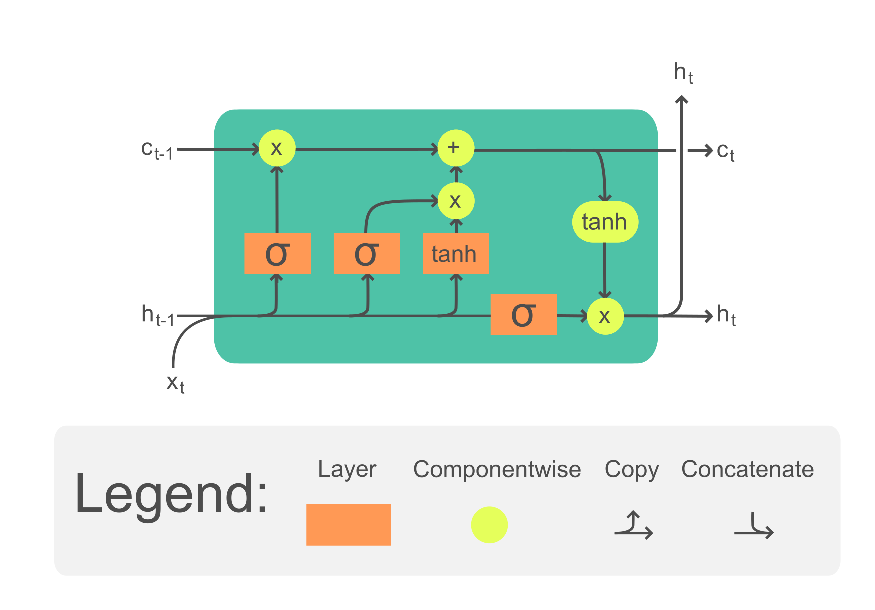
\includegraphics[width=0.7\linewidth]{figures/LSTM_Cell}
	\caption{LSTM cell,  From: \textcite{chevalier_english_2018}}
	\label{fig:lstmcell}
\end{figure}
When modelling soil temperature it is important to know the air temperatures at the previous hours or days to predict the next soil temperature time step, for this a natural selection for a data driven model is a recurrent network. This type of deep learning models makes prediction based on previous time steps in the data, however the longer timespan the model takes into account the less important are the earlier time-steps become according to the model. The LSTM model has been tried in Türkiye \cite{uluocak_daily_2024}, Belgium \cite{elmaz_cnn-lstm_2021}, United States of America \cite{li_modeling_2020} and their findings suggest it is a good model for predicting soil temperature, however it has also been used on a broader dateset spanning 3 continents \cite{li_attention-aware_2022}.

\acrshort{ac:lstm}\cite{hochreiter_long_1997} was developed in the field of Economy to predict the rise and fall of stocks, but has shown to be applicable to other problems that rely on time-series. It has been used to predict soil temperatures\cite{citakoglu_comparison_2017,elmaz_cnn-lstm_2021,feng_estimation_2019,kandasamy_performance_2023,li_attention-aware_2022,li_gans-lstm_2020,li_modeling_2020,wang_modeling_2022,mehdizadeh_modelling_2020} and utilizes a method of storing information across the timesteps to preserve information better when predicting, and sending information backwards during training so the earlier weights get adjusted more efficiently. This method is an attempt to solve the problem of the vanishing gradient problem.

The most common problem in training Neural networks is the vanishing gradient problem where updating the first few layers of a large network becomes exponentially more difficult since the adjustments gets smaller and smaller for each layer towards the start rather than the reverse. \gls{gl:lstm} changes this by carrying information from the previous cells forward thereby allowing updating earlier cells with bigger impact than the standard approach\cite{hochreiter_long_1997}. \acrshort{ac:lstm} is part of a family of \gls{gl:rnn}'s that passes information to other cells in the same layer.

LSTMs have proven effective in various tasks outside of economics such as natural language processing, speech recognition, and time series prediction. They provide a powerful mechanism for modeling sequential data while mitigating the vanishing gradient problem commonly encountered in basic RNNs.


\subsection{\acrfull{ac:gru}}

The complexity of soil temperatures and its dependency of previous time-steps make \gls{gl:rnn}'s a natural chose of a deep learning model, but the intricacy of an \acrshort{ac:lstm} makes it difficult to fine tune. An alternative to LSTM is the GRU model\cite{cho_learning_2014} that has fewer parameters to adjust however it has a memory mechanism that allows it to forget and remember information that is passes to other cells in the model. It has been used in Turkey\cite{uluocak_daily_2024}, and China\cite{li_forecasting_2024}

The \acrfull{ac:gru}\cite{cho_learning_2014} was developed in the field of natural language modeling to make translation predictions, however it has been shown that this model is also applicable in other applications than language translation. 

\acrshort{ac:gru} is a simplification of the LSTM cell with fewer total gates, and no output gate. This makes it quicker to train and better for memory deficient computers/servers.

GRU shares similarities with \acrshort{ac:lstm} networks but simplifies the architecture by using two gates: the update gate and the reset gate. These gates allow GRU to selectively retain relevant information from previous time steps while avoiding keeping unnecessary information. The update gate determines how much past information should be passed to the future, while the reset gate controls how much past information to forget. GRU has been effective in various sequence modeling tasks.
 
\begin{figure}[H]
	\centering
	\includegraphics[width = \textwidth]{figures/Gated_Recurrent_Unit_type_2.eps}
	\caption[GRU model sketch]{The GRU model where the memory cell gets more efficiently adjusted by the update gate (z) and appended information via the reset gate (r). From: \cite{jeblad_english_2018}}
\end{figure}

The GRU model offers several advantages over LSTM. It is smaller, converges more efficiently due to the integrated memory and prediction layer, and has fewer gates. These fewer tunable parameters make it faster to train and store the model weights.

\subsection{Bidirectional models}

\begin{figure}
	\centering
	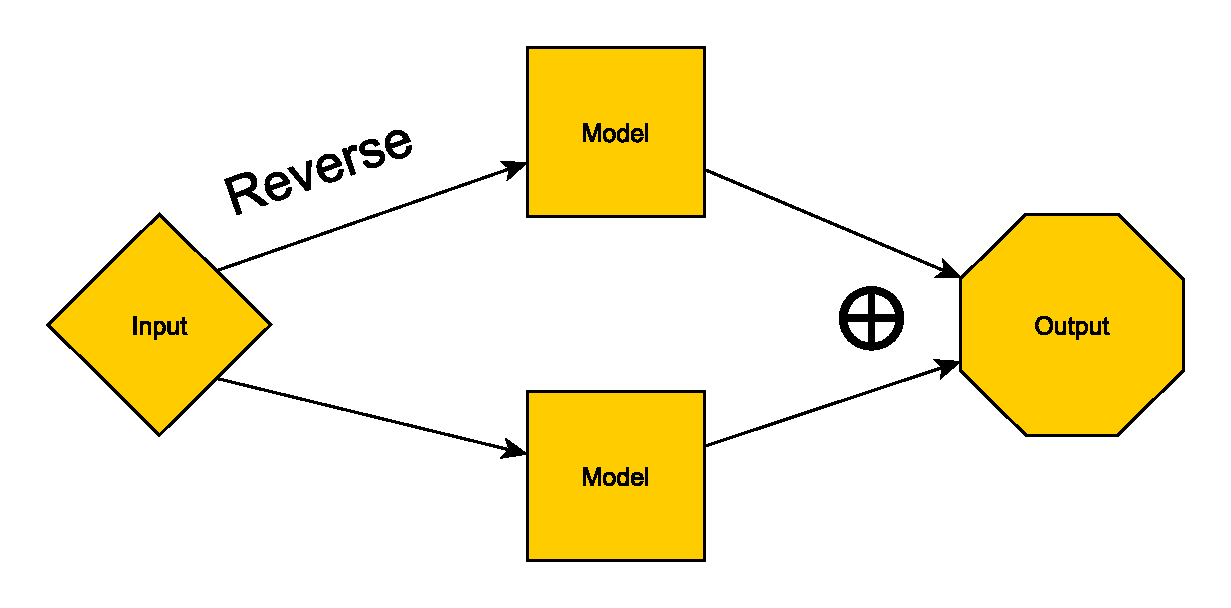
\includegraphics[width=0.8\linewidth]{figures/Bimodel}
	\caption[Bi-directional model diargam]{A diagram of the bidirectional method. The reverse indicates that the input data get reversed before it gets inserted into the model, while the bottom model gets the data. At the end the operator $\bigoplus$ get invoked that combines the output data from both model to a single output. The specifics of this operator can be any operation that combines two vectors to a single vector. In this study the operation is averaging the values.}
	\label{fig:bimodel}
\end{figure}

When making predictions with air temperatures as input, it would be useful not only to make predictions based only on air temperature from $t_0$ to $t_{max}$ since there is information to be found in the reverse time direction, $t_{max}$ to $t_0$. This technique has been applied in other studies with noteworthy performance increase, therefore will be used in this study for both LSTM model and GRU model using the TensorFlow Keras module. 

For the rest of the study a model with the prefix "Bi" indicates that it is a bidirectional model.


\section{Method}

\begin{figure}
	\centering
	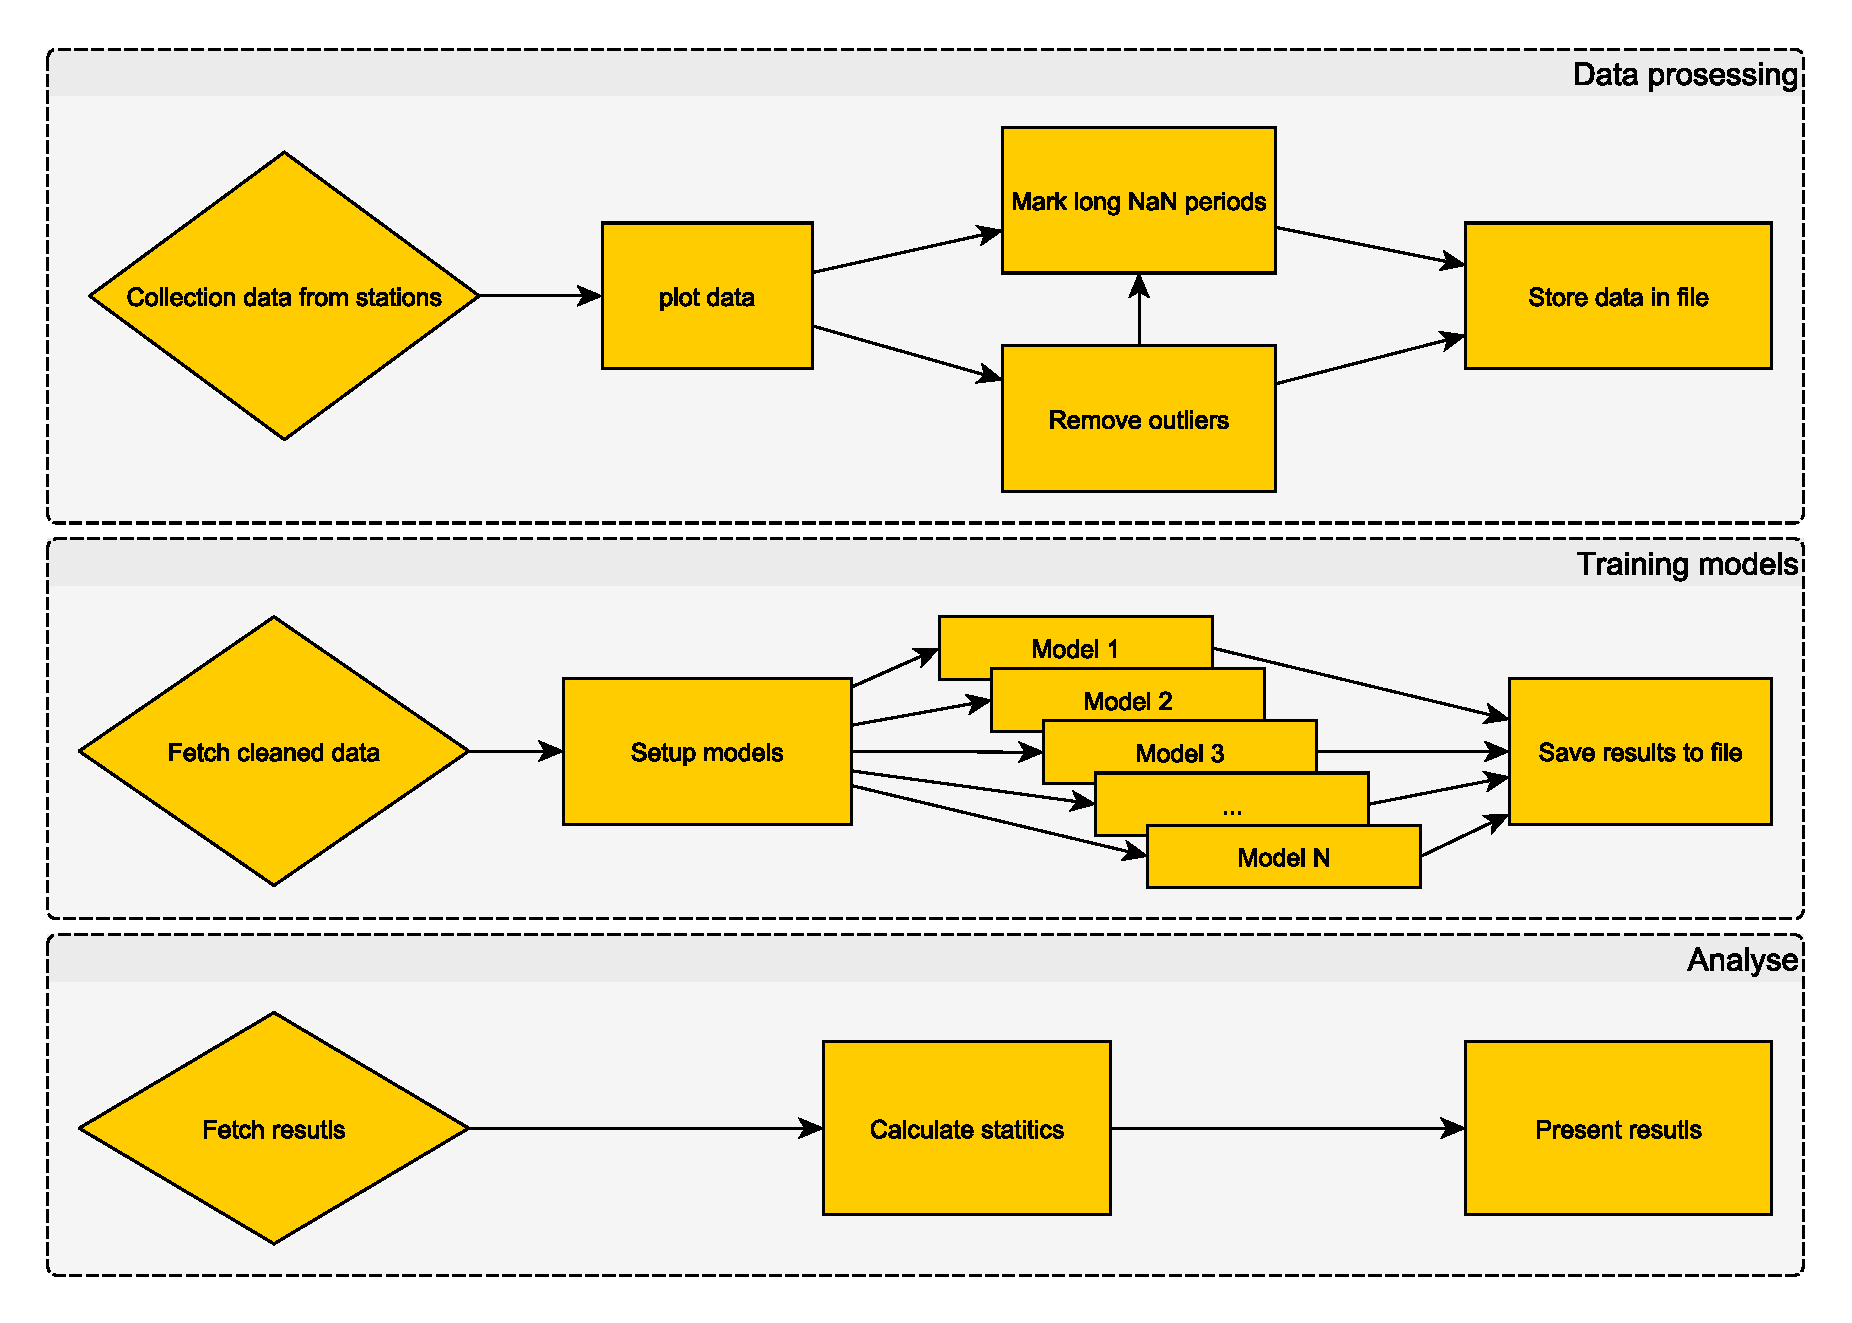
\includegraphics[width=0.7\linewidth]{figures/progress_diagram}
	\caption[Diagram sketching three procedures used in this study.]{A surface level diagram of the methodology.}
	\label{fig:progressdiagram}
\end{figure}

\subsection{Source of data}

For this comparative study the following data sources will be used

\begin{enumerate*}
	\item \acrfull{ac:nibio}
	\item \acrfull{ac:kilden}
	\item \acrfull{ac:met}
\end{enumerate*}

\subsection{Dataset}

The dataset is chosen from four regions in Norway; Innlandet, Vestfold, Trøndelag, and Østfold. From each region are four stations picked shown in table \ref{tab:station:names}
\begin{table}[h]
	\begin{adjustwidth}{-1in}{-1in}
		\centering
		\begin{tabular}{llrlrrrr}
			\hline Region&Name&ID&Drain type&MET name& Latitude&Longdetude&Altitude [m.a.s.l.]\\\hline
			Innlandet&Apelsvoll&11& Self-drained&SN11500&60,70024&10,86952&262\\
			Innlandet& Fåvang&17& Self-drained&SN13150&61,45822&10,18720&184\\
			Innlandet& Ilseng&26& Self-drained&SN12180&60,80264&11,20298&182\\
			Innlandet& Kise&27& Saturated&SN12550&60,77324&10,80569&129\\
			Trøndelag& Kvithamar&57& Saturated&SN69150&63,48795&10,87994&28\\
			Trøndelag& Frosta&15& Self-drained&SN69655&63,56502&10,69298&18\\
			Trøndelag& Mære&34& Self-drained&SN71320&63,94244&11,42527&59\\
			Trøndelag& Rissa&39& Saturated&SN71320&63,58569&9,97007&23\\
			Vestfold& Lier&30& Saturated&SN19940&59,79084&10,25962&38\\
			Vestfold& Sande&42& Saturated&SN26990&59,61620&10,22339&35\\
			Vestfold& Tjølling&50& Self-drained&SN27780&59,04641&10,12513&19\\
			Vestfold& Ramnes&38& Saturated&SN27315&59,38081&10,23970&39\\
			Østfold& Rakkestad&37& Saturated&SN3290&59,38824&11,39042&102\\
			Østfold& Rygge&41& Self-drained&SN17380&59,39805&10,75427&35\\
			Østfold& Tomb&52& Saturated&SN17050&59,31893&10,81449&12\\
			Østfold& Øsaker&118& Saturated&SN3370&59,31936&11,04221&45\\\hline
		\end{tabular}
	\end{adjustwidth}
	\caption[Staion information for each station/w location and MET-ID]{Station information from stations used in this study. The MET names was found by looking at the coordinates of the station and finding the closest MET station coordinates. \acrshort{ac:masl} stands for \acrlong{ac:masl}. The ID will be used in the text, tables, and figures for convenience and it was used in the code for something.}
	\label{tab:station:names}
\end{table}

% ™. These parameters were meticulously compiled from the Long-term Meteorological Trends (LMT) database, ensuring a robust dataset for evaluating temporal soil and air temperature patterns. This rich dataset provides valuable insights into the thermal dynamics of soil and air, which are essential for a multitude of ecological and agricultural applications.

The dataset created from all stations, spanning the period of 1st of March to 31st of October, annually from 2016 through 2022. This timeframe was selected to capture the critical growing seasons across various regions. The specific features extracted for analysis include the mean hourly soil temperature at a depth of 10cm (denoted as TJM10), the mean hourly soil temperature at 20cm (TJM20), and the mean hourly air temperature measured at 2 meters above ground level. These parameters were collected from the \acrfull{ac:kilden} database.

\subsubsection{Selection process}

An array of stations was provided by \acrshort{ac:kilden} based on their possession of the necessary data. All stations were reviewed, checked for missing data, and those with excessive gaps were removed from the list or replace with another station. After compiling a list of stations, each one was re-examined to identify outliers present in the data and eliminate them accordingly. If certain stations had an excessive number of missing values after the outlier check, nearby stations were sought, and the affected station was replaced and the outlier check was re-done. Table \ref{fig:plot-17} is showing Øsaker before treatment, and table \ref{fig:plot-17-treated} shows the same station cleaned and ready for being used as training/testing data.

\begin{figure}
		\centering
		\begin{adjustwidth}{-1in}{-1in}
			\includegraphics[height=0.7\textheight, width=1.35\textwidth]{"../../results/plots/Plot_test_naive_nan_k118_fTJM20.pdf"}
		\end{adjustwidth}
		\caption[Visual representation of Øsaker untreated]{Visual representation of missing values at Øsaker from 2014 to 2022 at the parameter "TJM20". The left numbers indicated how many hours that are missing and how many of them are shorter than or longer than 5 hours. The yellow markings indicate possible outliers based on the given year, all markings was checked if they were actual outliers. The red colouring indicate missing values in the data (represented in the data with code "NULL").}
		\label{fig:plot-17}
\end{figure}
\begin{figure}
		\centering
		\begin{adjustwidth}{-1in}{-1in}
			\includegraphics[height=0.7\textheight, width=1.35\textwidth]{"../../results/plots/Plot_test_naive_nan_treated_k118_fTJM20.pdf"}
		\end{adjustwidth}
		\caption[Visual representation of Øsaker treated]{Visual representation of missing values at Øsaker from 2014 to 2022 at the parameter "TJM20" after treating for outliers. The left numbers indicated how many hours that are missing and how many of them are longer or shorter than 5 hours, however for this visualization they indicate the untreated version of the data. The yellow markings indicate possible outliers based on the given year, all markings was checked if they were actual outliers. The red colouring indicate missing values in the data (represented in the data with code "NULL"). The years 2014 and 2015 was removed from the dataset but not coloured in due to technical limitations of reusable code, and furthermore half of 2016 was removed due to suspicion of misreading from sensor at this station.}
		\label{fig:plot-17-treated}
\end{figure}

The data plots (see figure \ref{fig:plot-17} and \ref{fig:plot-17-treated} as example) shows all the raw data plotted as a blue line from 03-01 to 10-31. The yellow markings is placed there by computer algorithmns (see section \ref{sec:method:outlier} for in-depth explanation of the outlier detection methods) as potential outliers in the data. These markings have been looked over and verified weather or not they are genuine outliers or not. Further more the red lines are indicators of missing values, the number of missing values longer or shorter than 5 hours\footnote{The threshold for rain is 3 hours due to the high variance.} are noted on the side bare with the total number of missing values regardless of length. The bottom bar are all the years laid on top of each other to highlight any years or periods that deviates for a particulate year compared to all the other years. There will be two versions of these plots, one for the untreated data and one for the treated data to show the difference the interpolation does to the data (see seciotn \ref{sec:method:interpolation} for further details.).

\subsubsection{Collection of data}

\begin{table}
	\centering
	\begin{tabular}{l|p{3cm}|p{3cm}}
		Name       &version&                       description                        \\ \hline
		PowerShell &7.3.11 & Windows native scripting language \\\hline
		Curl       & 8.4.0 (windows) libcurl/8.4.0 Schannel WinIDN & Command line tool to communicate with servers using http. \\\hline
		Python     &                    3.9.11                     &                popular Scripting language
	\end{tabular}
	\caption[software version description]{The description the software used in this study}
	\label{tab:software}
\end{table}

In the tabel \ref{tab:software} are the software programs used in this study and in the collection and treatment of the data. The program used in the collection of meteorological measurements is PowerShell in combination with Curl. Using hyperlinks gathered from inspecting \acrshort{ac:kilden}'s web page using the browser (Microsoft Edge) built-in inspector tool to get the relevant links to send data requests. The presise URL's can be reviewed on GitHub in the studies GitHub repository\footnote{Link: https://github.com/ConAltDelete/MT24CS}. For a more surfac level description on what was requested of the servers see table \ref{tab:station_request}.

\begin{table}
	\centering
	\begin{tabular}{r|p{5cm}|}
		FROST & Description\\ \hline
		Station ID & Sendt a request to LMT for station information using their remote API.\\
		 \hline LMT & Description\\ \hline
		Meteorological data & Requested soil temperature from 10cm depth, and 20cm depth and air temperature (2m), from 2014-03-01 to 2022-10-31.
	\end{tabular}
	\caption[Request to servers about stations]{Description of what was requested from each server (\acrshort{ac:met}, \acrshort{ac:nibio}).}
	\label{tab:station_request}
\end{table}

\subsubsection{Storage of data}
The storage of the data is done through two data structures; \gls{gl:hashmap} and \gls{gl:dataframe} from the package pandas. The transformation of data is done with a customized data-type called "DataFileHandler" which is converted to a module for convenience. The keys for the hashmap is chosen by the naming of the data files and the pattern given to the class. To escalate the loading of the data it will also be exported to a binary file for faster retrieval. 

\paragraph[Data structure]{Technical overview of custom data structure}
The data structure used to store the data from the different stations is called "DataFileHandler" and stores the data in a nested dictionary which can be interpreted as the data structure "tree". The main features of "DataFileHandler" is 
\begin{enumerate}
	\item Simple syntax for partitioning the data
	\item Grouping the data after loading
	\item Transforming all the data with the same function
	\item loading and unloading of a large collection of data
\end{enumerate}

This tree-structure uses recursion to search the dictonary to find the appropriate dataset to output. 

\subsection{Data cleaning and treatment}

To use the data in this study it must be cleaned and treated for training. Though the data has been examined by the supplier, however it still had outliers that needed to be treated before modelling. For this reason several steps and methods is utilized in the prepossessing steps. The selection process for finding these station can be compiled into these steps

\begin{enumerate}
	\item Recommendation from Norwegian Institute of Bio-economy Research
	\item \label{list:na_anal}Find the missing values in the data using algorithm \ref{alg:find_non_NULL_ranges_abstract}
	\item Analyse missing values 
	\item Searching LMT database for alternative station candidates if current data is insufficient
	\item If some station was replaced the repeat step \ref{list:na_anal}
\end{enumerate}

\subsubsection{Outlier detection and removal}\label{sec:method:outlier}

Though the data fetched from \acrshort{ac:nibio} is treated and controlled the external data from \acrshort{ac:met} might not be, and this research project incorporated raw, untreated data from \acrshort{ac:nibio} to fill inn missing values.

The method to quickly find obvious outliers was to look at the following z-score condition
\begin{equation}
	|z(|\Delta T|)| = \left|\frac{|\Delta T|-E(|\Delta T|)}{\sqrt{Var(|\Delta T|)}}\right|> 2.35.\label{eq:zscore}
\end{equation}

Where $ E() $ represents the expected value, which is a measure of the average of a set, $ Var() $ denotes the variance, which quantifies the spread or dispersion of the data points around the mean. The condition in equation \ref{eq:zscore} examines the absolute difference between successive measurements to compute the z-score for each data point then checks if it excised a score of 2.35, which translates to a check if a point performs a jump that deviates more than top $\sim 1\%$ of all the other data points that year. 

% determining if an observation exhibits a deviation that exceeds the threshold corresponding to approximately the top 1% of all data points within that year, thereby identifying significant anomalies.

The z-score is a statistical measure that normalizes the dataset. It is calculated by subtracting the mean from an individual data point and then dividing the result by the standard deviation. This process transforms the data so that the new mean of the dataset is 0 and the standard deviation is 1. By converting data to z-scores, also known as standard scores, it becomes easier to compare different datasets and identify outliers, as the data is now on a standardized scale. This technique is particularly useful in fields like finance, research, and quality control where relative comparisons are essential. 

The premise behind temperature analysis assumes that temperature fluctuations should be bounded, limiting how much they change from one time step to the next. To identify potential anomalies, an additional technique employed is the "out of line" method. This approach involves the program determining a projected point, denoted as $ C^* $, and then quantifying the deviation of the actual observed data point from this projection. For a graphical illustration of this method, refer to figure \ref{fig:localoutlier}, which visually depicts the extent of deviation of an observed temperature from its expected temperature. 

\begin{figure}[H]
	\centering
	\definecolor{zzttqq}{rgb}{0.6,0.2,0.}
	\definecolor{REDDD}{rgb}{0.8,0.5,0.2}
	\definecolor{ududff}{rgb}{0.3,0.3,1.}
	\begin{tikzpicture}[line cap=round,line join=round,>=triangle 45,x=1.0cm,y=1.0cm]
		\begin{axis}[
			x=1.0cm,y=1.0cm,
			axis lines=middle,
			ymajorgrids=true,
			xmajorgrids=true,
			xmin=-0.5,
			xmax=3.5,
			ymin=-0.5,
			ymax=2.5,
			xtick={-0.0,1.0,...,3.0},
			ytick={-0.0,1.0,...,2.0},]
			\clip(-0.5,-0.5) rectangle (3.5,2.5);
			\draw [line width=2.pt,dash pattern=on 1pt off 1pt] (1.04,1.02)-- (3.04,0.02);
			\draw [line width=2.pt] (1.04,1.02)-- (2.04,2.02);
			\draw [line width=2.pt] (2.04,2.02)-- (3.04,0.02);
			\begin{scriptsize}
				\draw [fill=ududff] (1.04,1.02) circle (2.5pt);
				\draw[color=ududff] (1.18,1.39) node {$A$};
				\draw [fill=ududff] (3.04,0.02) circle (1.5pt);
				\draw[color=ududff] (3.18,0.31) node {$B$};
				\draw [fill=ududff] (2.04,2.02) circle (1.5pt);
				\draw[color=ududff] (2.18,2.31) node {$C$};
				\draw [fill=zzttqq] (2.,0.54) circle (2.5pt);
				\draw [color=REDDD,dashed] (2.,0.54) circle (0.5);
				\draw[color=zzttqq] (2.14,0.91) node {$C^*$};
			\end{scriptsize}
		\end{axis}
	\end{tikzpicture}
	\caption[Simple Interpolation outlier detection]{An simple outlier detection method utilizing a simple line to estimate where the expected point ($C^*$,red dotted circle) is supposed to be. If observed point C falls outside the tolerance level (green circle) then it is marked as an outlier.}
	\label{fig:localoutlier}
\end{figure}

\subsubsection{Missing value imputation}\label{sec:method:interpolation}

The data has missing values, however it is still possible to impute some reasonable values that does not deviate too much from what is expected. When interpolating values the method chosen is a linear interpolation with a maximum period of 5 consecutive hours for soil temperatures, and 3 consecutive hours for air temperatures. The reasoning for this is that the soil temperatures are more reliable making it safer to interpolate without loosing too much information, while air temperatures has a higher variance making it more difficult to interpolate without cutting values. Due to a technical oversight in the coding of this study some large periods that should not be imputed get interpolated at the beginning of the interval.

\subsubsection{Summary of data}

Following the processes of outlier removal and missing value interpolation, the statistics for the refined dataset are presented in table \ref{tab:staion:summary:overall}. For an in-depth year-by-year breakdown, please refer to the summaries located in appendix \ref{apx:tables:station:summary}.

\begin{table}[H]
	\begin{adjustwidth}{-1in}{-1in}
		\centering
		\begin{tabular}{rlll}
\hline
   station ID & TM [℃]   & TJM10 [℃]   & TJM20 [℃]   \\
\hline
           50 & \begin{tabular}{ll}
\hline
 $\mu$:11.43   & max:31.3  \\
 $\sigma$:6.16 & min:-14.0 \\
\hline
\end{tabular}          & \begin{tabular}{ll}
\hline
 $\mu$:11.11   & max:21.9 \\
 $\sigma$:5.35 & min:-0.3 \\
\hline
\end{tabular}             & \begin{tabular}{ll}
\hline
 $\mu$:10.71   & max:19.3 \\
 $\sigma$:5.16 & min:0.0  \\
\hline
\end{tabular}             \\
           42 & \begin{tabular}{ll}
\hline
 $\mu$:11.04   & max:33.0  \\
 $\sigma$:6.83 & min:-14.5 \\
\hline
\end{tabular}          & \begin{tabular}{ll}
\hline
 $\mu$:11.27   & max:23.2 \\
 $\sigma$:5.93 & min:-0.4 \\
\hline
\end{tabular}             & \begin{tabular}{ll}
\hline
 $\mu$:11.16   & max:20.6 \\
 $\sigma$:5.62 & min:-0.1 \\
\hline
\end{tabular}             \\
           38 & \begin{tabular}{ll}
\hline
 $\mu$:11.11   & max:32.3  \\
 $\sigma$:6.81 & min:-19.7 \\
\hline
\end{tabular}          & \begin{tabular}{ll}
\hline
 $\mu$:11.13   & max:22.8 \\
 $\sigma$:5.89 & min:0.1  \\
\hline
\end{tabular}             & \begin{tabular}{ll}
\hline
 $\mu$:10.96   & max:21.7 \\
 $\sigma$:5.71 & min:0.3  \\
\hline
\end{tabular}             \\
           30 & \begin{tabular}{ll}
\hline
 $\mu$:11.11   & max:32.5  \\
 $\sigma$:6.92 & min:-16.8 \\
\hline
\end{tabular}          & \begin{tabular}{ll}
\hline
 $\mu$:11.24   & max:27.6 \\
 $\sigma$:5.98 & min:-3.3 \\
\hline
\end{tabular}             & \begin{tabular}{ll}
\hline
 $\mu$:11.14   & max:23.5 \\
 $\sigma$:5.66 & min:-3.3 \\
\hline
\end{tabular}             \\
          118 & \begin{tabular}{ll}
\hline
 $\mu$:11.15   & max:33.1  \\
 $\sigma$:6.61 & min:-16.6 \\
\hline
\end{tabular}          & \begin{tabular}{ll}
\hline
 $\mu$:10.61   & max:21.8 \\
 $\sigma$:5.47 & min:-0.9 \\
\hline
\end{tabular}             & \begin{tabular}{ll}
\hline
 $\mu$:10.42   & max:20.3 \\
 $\sigma$:5.22 & min:-0.7 \\
\hline
\end{tabular}             \\
           52 & \begin{tabular}{ll}
\hline
 $\mu$:11.01   & max:32.6  \\
 $\sigma$:6.78 & min:-18.0 \\
\hline
\end{tabular}          & \begin{tabular}{ll}
\hline
 $\mu$:11.71   & max:23.2 \\
 $\sigma$:5.51 & min:-1.0 \\
\hline
\end{tabular}             & \begin{tabular}{ll}
\hline
 $\mu$:11.67   & max:24.2 \\
 $\sigma$:5.41 & min:-0.6 \\
\hline
\end{tabular}             \\
           41 & \begin{tabular}{ll}
\hline
 $\mu$:11.24   & max:33.7  \\
 $\sigma$:6.68 & min:-19.2 \\
\hline
\end{tabular}          & \begin{tabular}{ll}
\hline
 $\mu$:11.65   & max:25.9 \\
 $\sigma$:6.02 & min:-0.8 \\
\hline
\end{tabular}             & \begin{tabular}{ll}
\hline
 $\mu$:11.32  & max:22.2 \\
 $\sigma$:5.7 & min:-0.3 \\
\hline
\end{tabular}             \\
           37 & \begin{tabular}{ll}
\hline
 $\mu$:10.15   & max:31.6  \\
 $\sigma$:6.84 & min:-20.1 \\
\hline
\end{tabular}          & \begin{tabular}{ll}
\hline
 $\mu$:10.59   & max:22.0 \\
 $\sigma$:5.58 & min:-1.5 \\
\hline
\end{tabular}             & \begin{tabular}{ll}
\hline
 $\mu$:10.49   & max:20.5 \\
 $\sigma$:5.46 & min:-0.7 \\
\hline
\end{tabular}             \\
           39 & \begin{tabular}{ll}
\hline
 $\mu$:9.62    & max:31.4  \\
 $\sigma$:5.94 & min:-15.1 \\
\hline
\end{tabular}          & \begin{tabular}{ll}
\hline
 $\mu$:9.29   & max:19.6 \\
 $\sigma$:4.9 & min:-0.9 \\
\hline
\end{tabular}             & \begin{tabular}{ll}
\hline
 $\mu$:9.18    & max:18.5 \\
 $\sigma$:4.79 & min:-0.3 \\
\hline
\end{tabular}             \\
           34 & \begin{tabular}{ll}
\hline
 $\mu$:9.34    & max:32.7  \\
 $\sigma$:6.55 & min:-19.5 \\
\hline
\end{tabular}          & \begin{tabular}{ll}
\hline
 $\mu$:8.79   & max:19.3 \\
 $\sigma$:4.9 & min:-1.3 \\
\hline
\end{tabular}             & \begin{tabular}{ll}
\hline
 $\mu$:8.69    & max:17.9 \\
 $\sigma$:4.73 & min:-0.2 \\
\hline
\end{tabular}             \\
           57 & \begin{tabular}{ll}
\hline
 $\mu$:9.73    & max:32.8  \\
 $\sigma$:6.41 & min:-21.4 \\
\hline
\end{tabular}          & \begin{tabular}{ll}
\hline
 $\mu$:9.39    & max:22.2 \\
 $\sigma$:5.23 & min:-1.3 \\
\hline
\end{tabular}             & \begin{tabular}{ll}
\hline
 $\mu$:9.13    & max:19.1 \\
 $\sigma$:5.07 & min:-0.9 \\
\hline
\end{tabular}             \\
           15 & \begin{tabular}{ll}
\hline
 $\mu$:10.07  & max:33.5  \\
 $\sigma$:6.1 & min:-15.4 \\
\hline
\end{tabular}          & \begin{tabular}{ll}
\hline
 $\mu$:9.19    & max:20.2 \\
 $\sigma$:4.76 & min:-0.2 \\
\hline
\end{tabular}             & \begin{tabular}{ll}
\hline
 $\mu$:9.07   & max:18.7 \\
 $\sigma$:4.6 & min:0.0  \\
\hline
\end{tabular}             \\
           27 & \begin{tabular}{ll}
\hline
 $\mu$:9.97    & max:33.0  \\
 $\sigma$:6.99 & min:-23.2 \\
\hline
\end{tabular}          & \begin{tabular}{ll}
\hline
 $\mu$:10.55   & max:23.9 \\
 $\sigma$:6.25 & min:-2.7 \\
\hline
\end{tabular}             & \begin{tabular}{ll}
\hline
 $\mu$:10.21   & max:21.4 \\
 $\sigma$:5.97 & min:-2.2 \\
\hline
\end{tabular}             \\
           26 & \begin{tabular}{ll}
\hline
 $\mu$:9.64    & max:32.4  \\
 $\sigma$:7.31 & min:-26.3 \\
\hline
\end{tabular}          & \begin{tabular}{ll}
\hline
 $\mu$:9.53    & max:22.6 \\
 $\sigma$:6.17 & min:-3.0 \\
\hline
\end{tabular}             & \begin{tabular}{ll}
\hline
 $\mu$:9.51   & max:20.6 \\
 $\sigma$:6.1 & min:-2.2 \\
\hline
\end{tabular}             \\
           17 & \begin{tabular}{ll}
\hline
 $\mu$:9.19    & max:29.9  \\
 $\sigma$:7.63 & min:-25.9 \\
\hline
\end{tabular}          & \begin{tabular}{ll}
\hline
 $\mu$:9.64    & max:22.8 \\
 $\sigma$:6.44 & min:-2.4 \\
\hline
\end{tabular}             & \begin{tabular}{ll}
\hline
 $\mu$:9.35    & max:19.9 \\
 $\sigma$:6.09 & min:-1.4 \\
\hline
\end{tabular}             \\
           11 & \begin{tabular}{ll}
\hline
 $\mu$:9.76   & max:30.2  \\
 $\sigma$:6.9 & min:-21.4 \\
\hline
\end{tabular}          & \begin{tabular}{ll}
\hline
 $\mu$:10.15   & max:23.3 \\
 $\sigma$:6.17 & min:-1.6 \\
\hline
\end{tabular}             & \begin{tabular}{ll}
\hline
 $\mu$:10.0    & max:21.6 \\
 $\sigma$:5.91 & min:-1.1 \\
\hline
\end{tabular}             \\
\hline
\end{tabular}
	\end{adjustwidth}
	\caption[Table of station statistics]{The table shows the statistics of each station for each feature except for Time as it is a strictly monotonic sequence. The station names can be found in table \ref{tab:station:names}. $\mu$ Denotes the mean temperature, $\sigma$ denotes the standard deviation, "min" is the minimum temperature, and "max" is the maximum temperature. All values in the table have the unit degree Celsius.}
	\label{tab:staion:summary:overall}
\end{table}

\subsection{Setup of models}

The models are set up in according to the relevant paper the model is fetched from, alternatively reuse the code made by the author. When importing the data to the model there will be modifying to the original code to facilitate for the model as far as it goes. Any modifications will be in the appendix under section \ref{apx:code}. For the convenience of the reader all code is using the sklearn estimator class to make all the models discuses in this study more user friendly and compatible with sklearns other functions. The details of the models will be discussed in section \ref{sec:theory}, this section discusses the setup and implementation of the models.\footnote{Caution to the reader; The code used was run on the Linux subsystem (Debian) on windows due to the fact that the current version of tensorflow can't run on Windows.}

\subsubsection{Basic Linear model}

The linear model (section \ref{sec:theory:linreg}) utilises in the study is created from the python model sklearn (or scikit-learn according to pythons package manager). The model is setup with standard parameters, and the data is fed into the model without scaling with fitted intercept coefficient. 

\subsubsection{Plauborg}

The Plauborg regression will be formulated as a Linear Regression problem so that the 'LinearRegression' function in the Sci-kit module can be used. For the parameters used in the paper\cite{plauborg_simple_2002} the F function defined in section \ref{sec:theory:pluborg} will be formulated with loops to give rise 3 more parameters for fine-tuning the model. NULL-values generated from the procedure get replaced with 0, since the data fed to the model is significantly larger than 10h (the minimum for the training is 24h).

\subsubsection{LSTM}

The LSTM used in this study came from the keras module using standard settings.

\begin{table}
	\centering
	\begin{tabular}{l|l|l|l}
		Parameter&value&Parameter&value\\\hline
		activation&"tanh"&kernel\_constraint&None\\
		recurrent\_activation&"sigmoid"&recurrent\_constraint&None\\
		use\_bias&True&bias\_constraint&None\\
		kernel\_initializer&"glorot\_uniform"&dropout&0.0\\
		recurrent\_initializer&"orthogonal"&recurrent\_dropout&0.0\\
		bias\_initializer&"zeros"&seed&None\\
		unit\_forget\_bias&True&return\_sequences&False\\
		kernel\_regularizer&None&return\_state&False\\
		recurrent\_regularizer&None&go\_backwards&False\\
		bias\_regularizer&None&stateful&False\\
		activity\_regularizer&None&unroll&False\\
		use\_cudnn&"auto"&&
	\end{tabular}
	\caption[LSTM standard paramters]{All the hyperparameters that are available to the Keras LSTM Layer and the standard options that this study chose to remain unchanged}
	\label{tab:lstm:params}
\end{table}

\subsubsection{GRU}

The GRU model used in this study is fetched from TensorFlow-Keras python module with standard settings. The model class used in this study is the Keras default GRU layer. The model settings can be reviewed in table \ref{tab:gru:params} which is the standard settings for the keras class.

\begin{table}
	\centering
	\begin{tabular}{l|l|l|l}
		Parameter&value&Parameter&value\\\hline
		activation&"tanh"&recurrent\_constraint&None\\
		recurrent\_activation&"sigmoid"&bias\_constraint&None\\
		use\_bias&True&dropout&0.0\\
		kernel\_initializer&"glorot\_uniform"&recurrent\_dropout&0.0\\
		recurrent\_initializer&"orthogonal"&seed&None\\
		bias\_initializer&"zeros"&return\_sequences&False\\
		kernel\_regularizer&None&return\_state&False\\
		recurrent\_regularizer&None&go\_backwards&False\\
		bias\_regularizer&None&stateful&False\\
		activity\_regularizer&None&unroll&False\\
		kernel\_constraint&None&reset\_after&True\\
		use\_cudnn&"auto"&&
	\end{tabular}
	\caption[GRU standard parameters]{All the hyperparameters that are available to the Keras GRU Layer and the standard options that this study chose to remain unchanged}
	\label{tab:gru:params}
\end{table}

\subsubsection{Bidirectional layer}

The Bi-directional layer used in this study came from the keras module using standard settings except for "merge\_mode" which is set to "ave" for averaging the output values. This was done since there are no other layers to get those values. The table of configurations can be found in table \ref{tab:bidir:params}.

\begin{table}
	\centering
	\begin{tabular}{l|l}
		Parameter&value\\\hline
		merge\_mode&"ave"\\
		weights&None\\
		backward\_layer&None
	\end{tabular}
	\caption[Bidirectional method parameters]{The adjustable parameters of the bidirectional layer from Keras.}
	\label{tab:bidir:params}
\end{table}


\subsection{Metrics}\label{sec:method:metric}

The metrics used in this study are

\begin{itemize*}
	\item \acrfull{ac:rmse}
	\item \acrfull{ac:mae}
	\item \acrfull{ac:r2}
	\item Bias
	\item \acrfull{ac:kappa}
	\item digit sensitivity
\end{itemize*}

Soil temperature as a different behaviour than air temperature since energy (temperature) though the soil gets dampen and delayed. Since the data used in this study has outliers that was not caught during data treatment, which has been addressed, the author of this study decided to include two more metrics that are not usually included in the evaluation; The log condition number, and digit sensitivity. Both metrics are based on the calculation of the condition number defined in formula \ref{eq:kappa}.

\begin{equation}\label{eq:kappa}
\kappa = \lim\limits_{\varepsilon \to 0^+} \sup\limits_{|\partial x|\leq\varepsilon}  \frac{\left|f(x+\partial x) - f(x)\right|}{|f(x)|}*\frac{|x|}{|\partial x|} 
\end{equation}

Calculating this directly is impossible due to the limitations of handling infinitesimally small numbers in simulations. However, this paper uses a own designed algorithm (referred to as $\kappa$) to estimate this value for all the models. See algorithm \ref{alg:cond_num} for the pseudocode of the algorithm.

\begin{algorithm}[H]
	\SetAlgoLined
	\KwData{ Data }
	\KwResult{log($\kappa$)}
	Let $\kappa_f$ be the function \ref{eq:kappa}\;
	$\kappa\gets 0$\;
	\For{$i \in {1 \dots |Data|}$}{
		$\partial x \gets \mathcal{U}_{[-\sqrt{\varepsilon/|Data|},\sqrt{\varepsilon/|Data|}]}$\;
		$k \gets$ calculate with $\kappa_f$ from $x$ and $x+\partial x$\;
		\If{k > $\kappa$}{$\kappa \gets k$\;}
	}
	\Return{$\kappa$}
	\caption[Randommised $\kappa$ algorithm]{Method for calculating $\kappa$. $\mathcal{U}$ is a uniform random distribution in a range.}
	\label{alg:cond_num}
\end{algorithm}

The normal use case for $\kappa$ is to check the sensitivity of matrices for small changes in the input,  

The digit sensitivity is included to give an intuitive understanding of $\kappa$ and is computed simply as $\log_e(\kappa)+1$. This number tells us the significant digit generated from the model. If the number is less than 0 then it's the nth digit after the decimal point.

For the rest of the metrics, they are defined as follows
\begin{itemize}
	\item \gls{ac:rmse} \begin{equation}\sqrt{\frac{\sum (y_{\text{pred}} - y_{\text{truth}})^2}{n}}\end{equation}
	\item \gls{ac:mae} \begin{equation}\frac{\sum \left| y_{\text{pred}} - y_{\text{truth}}\right|}{n}\end{equation}
	\item bias \begin{equation}\frac{\sum ( y_{\text{pred}} - y_{\text{truth}})}{n}\end{equation}
	\item \gls{ac:r2} \begin{equation}1-\frac{\sum (y_{\text{pred}} - y_{\text{truth}})^2}{\sum (y_{\text{pred}} - \vec{y})^2}\end{equation}
\end{itemize}

Where $\vec{y}$ is the mean of the target, $y_{\text{pred}}$ is the predicted data, and $y_{\text{truth}}$ is the observed soil temperature.

\subsubsection{Confidence eclipses}\label{sec:method:eclipse}

To see goodness of fit to the ground truth (soil temperature) confidence eclipses will be calculated for the results. This is done by calculating the singular values of the predicted soil temperature and the observed ground truth. A way to define it would be with equation \eqref{eq:singval}.

\begin{equation}
	\left|\left[Y \quad \tilde{Y}\right]^T \left[Y \quad \tilde{Y}\right] -\lambda I\right| = 0\label{eq:singval}
\end{equation}

Where $Y$ is the soil temperature, $\tilde{Y}$ is the predicted soil temperature, $[\dots]^T$ is the transpose of a matrix, $\lambda$ is a diagonal matrix with the entries being the singular values, and $I$ is the identity matrix. The interpretation of the singular values would be the width and hight of the eclipse that covers 1 standard deviation of the data in two dimensions. In section \ref{sec:result} only the smallest singular value will be shown, denoted $\lambda_0$, as it will be half the width of the eclipse and will show if a model fits to the symmetry line. Furtermore, the figures of the confidence eclipses will also show 2nd standard deviation, and 3rd standard deviation for completeness. 

\subsection{Model training}

When training the model's data from 2014 to 2020 get used as the training data and the years 2021 to 2022 will be used as the test set. Normally data sets get split up into multiple training sets and test sets known as cross-validation however since this study have collected a large amount of data this technique is not necessary for the analyses. However, since the study utilizes the GridSearchCV class for finding optimal parameters cross-validation will be performed anyway within the training set by default.

The models get trained on air temperature, however the precise input for each model is not the same for all. The features used for each model are described in table \ref{tab:model_trans} and their transformation in table \ref{tab:model_trans}.

The models get a sample of the training data at the time due to the size and the amount for missing data (for example figure \ref{fig:plot-17}) The algorithm used to fetch reliable indexes are demonstrated at algorithm \ref{alg:find_non_NULL_ranges_abstract}.

\begin{algorithm}
	\caption{Find Non-NULL Ranges (Abstract)}
	\label{alg:find_non_NULL_ranges_abstract}
	\SetKwFunction{FindNonNULLRanges}{FindNonNULLRanges}
	\SetKwInOut{Input}{Input}
	\SetKwInOut{Output}{Output}
	
	\Input{Input data $\text{data}$}
	\Output{List of tuples: $\text{ranges}$}
	
	\BlankLine
	\SetKwData{StartIdx}{start}
	\SetKwData{NonNULLRanges}{ranges}
	\SetKwData{Item}{item}
	
	\FindNonNULLRanges{$\text{data}$}{
		$\NonNULLRanges \gets$ empty list\;
		$\StartIdx \gets$ None\;
		
		\For{$\Item \text{ in } \text{data}$}{
			\If{$\Item is not NULL$}{
				\If{$\StartIdx \text{ is None}$}{
					$\StartIdx \gets \Item$\;
				}
			}
			\Else{
				\If{$\StartIdx \text{ is not None}$}{
					Add ($\StartIdx$, $\Item$ index - 1) to $\NonNULLRanges$\;
					$\StartIdx \gets$ None\;
				}
			}
		}
		\If{$\StartIdx \text{ is not None}$}{
			Add ($\StartIdx$, Last index) to $\NonNULLRanges$\;
		}
		\Return $\NonNULLRanges$\;
	}
\end{algorithm}

After the missing values has been identified rows get removed in such a way that if any of the features or target values is missing then that row get removed. At the end all the rows get concatenated , so there is just one complete dataset for the training. 

\begin{table}[H]
	\centering
	\begin{tabular}{|r|c|c| p{6cm}|}
		\hline Model name & features& target & transformations \\\hline\hline
		Linear Regression & TM& TJM10, TJM20 & --- \\\hline
		Plauborg & Time, TM& TJM10, TJM20 & Time get translated in two way; the current day since new year if looking at daily values, and hours since new year if looking at hourly predictions. When converting TM to daily values the hourly data get averaged in 24 hour periods from midnight to 23:00\\\hline
		Deep learning models &Time, TM& TJM10, TJM20& Time get translated to hours since new year by taking the day of the year and multiplying it by 24 and adding the hour.\\\hline
	\end{tabular}
	\caption[Model parameters]{Parameters used for predicting soil temperatures at depth 10cm and 20cm. The deep learning models encapsulated in the "Deep learing models" are LSTM, BiLSTM, GRU, and BiGRU.}
	\label{tab:model_trans}
\end{table}

\subsection[Use of AI]{Use of Artificial Intelligence in this paper}

In this paper there has been used Artificial Intelligence (AI), specifically Bing Chat / Copilot hosted by Microsoft Cooperation according to the current guidelines for use of artificial intelligence at the faculty of \acrfull{ac:nmbu}, for the following purposes:

\begin{enumerate}
	\item Formalizing sentences and rephrasing sentences.
	\item Spellchecking
	\item Code generation of basic consepts and structures (tree traversal, template for generic classes) 
\end{enumerate}

It is important to emphasize that my engagement with AI have been actively curated and verified with known sources. All code underwent rigorous manual inspection within a dedicated testing environment. Furthermore, no confidential or sensitive information was shared with the AI; my interactions focused solely on broad topics and general inquiries. To validate the accuracy of AI-generated responses, it has been cross-checked with established research papers and textbooks.


\section{Results}\todo{Summerize results}

\todo{Make sections}
\todo{Include tables}

\begin{table}
	\centering
	\begin{adjustwidth}{-1in}{-1in}
		\resizebox{1.35\textwidth}{!}{
			\begin{tabular}{llrrrrrrrrr}
\hline
 model                               &       &    52 &    37 &    50 &   38 &   57 &    34 &    27 &   17 &   average \\
\hline
 Linear model 10cm                   & $R^2$ &  0.22 &  0.47 &  0.58 & 0.39 & 0.3  & -1.39 &  0.55 & 0.5  &      0.42 \\
                                     & MAE   &  2.89 &  3.5  &  2.7  & 3.74 & 3.36 &  3.42 &  3.24 & 3.43 &      3.27 \\
                                     & RMSE  &  3.68 &  4.5  &  3.61 & 4.81 & 4.29 &  4.26 &  4.27 & 4.52 &      4.23 \\
                                     & bias  &  1.23 &  2.07 &  1.77 & 2.5  & 2.77 &  3.18 &  2.08 & 2.51 &      2.3  \\
 Plauborg model (daily values) 10cm  & $R^2$ &  0.66 &  0.87 &  0.94 & 0.85 & 0.85 &  0.4  &  0.9  & 0.88 &      0.86 \\
                                     & MAE   &  1.84 &  1.76 &  1.11 & 1.91 & 1.55 &  1.69 &  1.63 & 1.78 &      1.62 \\
                                     & RMSE  &  2.42 &  2.21 &  1.4  & 2.42 & 1.98 &  2.14 &  2.06 & 2.26 &      2.07 \\
                                     & bias  & -0.64 &  0.37 & -0.05 & 0.67 & 1.11 &  1.53 &  0.4  & 0.92 &      0.61 \\
 Plauborg model (hourly values) 10cm & $R^2$ &  0.64 &  0.86 &  0.88 & 0.75 & 0.68 & -0.19 &  0.87 & 0.83 &      0.79 \\
                                     & MAE   &  1.96 &  1.8  &  1.47 & 2.37 & 2.26 &  2.31 &  1.72 & 1.98 &      1.93 \\
                                     & RMSE  &  2.51 &  2.34 &  1.91 & 3.05 & 2.91 &  3.01 &  2.28 & 2.65 &      2.53 \\
                                     & bias  & -0.35 &  0.24 &  0.56 & 1.36 & 0.68 &  0.85 &  0.16 & 0.06 &      0.6  \\
 BiLSTM 10cm                         & $R^2$ &  0.75 &  0.96 &  0.96 & 0.95 & 0.92 &  0.69 &  0.95 & 0.95 &      0.93 \\
                                     & MAE   &  1.48 &  1.01 &  0.86 & 1.03 & 1.11 &  1.17 &  1.13 & 1.11 &      1.11 \\
                                     & RMSE  &  2.08 &  1.22 &  1.06 & 1.43 & 1.4  &  1.56 &  1.36 & 1.4  &      1.42 \\
                                     & bias  & -1.08 & -0.17 & -0.48 & 0.18 & 0.42 &  0.75 & -0.11 & 0.46 &      0.06 \\
 LSTM 10cm                           & $R^2$ &  0.71 &  0.92 &  0.94 & 0.89 & 0.86 &  0.52 &  0.91 & 0.92 &      0.89 \\
                                     & MAE   &  1.72 &  1.49 &  1.11 & 1.48 & 1.46 &  1.47 &  1.56 & 1.43 &      1.47 \\
                                     & RMSE  &  2.25 &  1.77 &  1.39 & 2.01 & 1.91 &  1.92 &  1.89 & 1.81 &      1.87 \\
                                     & bias  & -0.81 &  0.02 & -0.05 & 0.54 & 0.55 &  0.88 &  0.04 & 0.46 &      0.3  \\
 GRU 10cm                            & $R^2$ &  0.7  &  0.91 &  0.93 & 0.89 & 0.91 &  0.64 &  0.91 & 0.9  &      0.89 \\
                                     & MAE   &  1.69 &  1.53 &  1.18 & 1.57 & 1.19 &  1.31 &  1.49 & 1.54 &      1.42 \\
                                     & RMSE  &  2.29 &  1.89 &  1.44 & 2    & 1.5  &  1.69 &  1.85 & 1.98 &      1.81 \\
                                     & bias  & -1.19 & -0.15 & -0.72 & 0.02 & 0.59 &  1.03 & -0.14 & 0.5  &      0.03 \\
 BiGRU 10cm                          & $R^2$ &  0.69 &  0.93 &  0.95 & 0.92 & 0.88 &  0.62 &  0.92 & 0.93 &      0.9  \\
                                     & MAE   &  1.69 &  1.37 &  1.05 & 1.34 & 1.38 &  1.34 &  1.44 & 1.31 &      1.36 \\
                                     & RMSE  &  2.31 &  1.66 &  1.29 & 1.78 & 1.74 &  1.73 &  1.77 & 1.69 &      1.72 \\
                                     & bias  & -1.15 & -0.31 & -0.4  & 0.23 & 0.23 &  0.55 & -0.3  & 0.08 &     -0.04 \\
\hline
\end{tabular}
		}
	\end{adjustwidth}
\end{table}


\begin{table}
	\centering
	\begin{adjustwidth}{-1in}{-1in}
		\resizebox{1.35\textwidth}{!}{
			\begin{tabular}{llrrrrrrrrr}
\hline
 model                               &       &    41 &   118 &    42 &    30 &   39 &    15 &   26 &    11 &   average \\
\hline
 Linear model 10cm                   & $R^2$ &  0.59 &  0.31 &  0.51 &  0.59 & 0.21 & -0    & 0.46 &  0.51 &      0.42 \\
                                     & MAE   &  3.07 &  3.49 &  3.52 &  3.11 & 3.19 &  3.14 & 3.65 &  2.71 &      3.27 \\
                                     & RMSE  &  3.98 &  4.5  &  4.57 &  4.05 & 4.06 &  3.92 & 4.71 &  3.57 &      4.23 \\
                                     & bias  &  1.49 &  2.93 &  2.11 &  1.73 & 2.83 &  2.8  & 2.9  &  1.53 &      2.3  \\
 Plauborg model (daily values) 10cm  & $R^2$ &  0.9  &  0.84 &  0.88 &  0.91 & 0.83 &  0.79 & 0.86 &  0.86 &      0.86 \\
                                     & MAE   &  1.59 &  1.7  &  1.75 &  1.52 & 1.46 &  1.43 & 1.94 &  1.5  &      1.62 \\
                                     & RMSE  &  1.98 &  2.17 &  2.24 &  1.91 & 1.9  &  1.81 & 2.43 &  1.88 &      2.07 \\
                                     & bias  & -0.29 &  1.14 &  0.33 & -0.05 & 1.19 &  1.11 & 1.25 &  0.34 &      0.61 \\
 Plauborg model (hourly values) 10cm & $R^2$ &  0.9  &  0.71 &  0.85 &  0.89 & 0.63 &  0.56 & 0.84 &  0.82 &      0.79 \\
                                     & MAE   &  1.52 &  2.32 &  1.88 &  1.55 & 2.15 &  1.99 & 1.92 &  1.67 &      1.93 \\
                                     & RMSE  &  1.94 &  2.93 &  2.5  &  2.07 & 2.77 &  2.59 & 2.53 &  2.15 &      2.53 \\
                                     & bias  &  0.15 &  1.64 &  0.7  &  0.35 & 0.7  &  0.9  & 0.82 &  0.04 &      0.6  \\
 BiLSTM 10cm                         & $R^2$ &  0.94 &  0.94 &  0.95 &  0.95 & 0.88 &  0.89 & 0.95 &  0.93 &      0.93 \\
                                     & MAE   &  1.2  &  1.07 &  1.1  &  1.13 & 1.24 &  1.02 & 1.2  &  1.08 &      1.11 \\
                                     & RMSE  &  1.47 &  1.32 &  1.4  &  1.44 & 1.59 &  1.3  & 1.49 &  1.34 &      1.42 \\
                                     & bias  & -0.76 &  0.64 & -0.17 & -0.56 & 0.5  &  0.44 & 0.74 & -0.12 &      0.06 \\
 LSTM 10cm                           & $R^2$ &  0.91 &  0.88 &  0.9  &  0.91 & 0.83 &  0.8  & 0.91 &  0.87 &      0.89 \\
                                     & MAE   &  1.54 &  1.41 &  1.59 &  1.52 & 1.4  &  1.37 & 1.58 &  1.5  &      1.47 \\
                                     & RMSE  &  1.85 &  1.87 &  2    &  1.88 & 1.85 &  1.75 & 1.96 &  1.85 &      1.87 \\
                                     & bias  & -0.37 &  1.05 &  0.2  & -0.18 & 0.62 &  0.67 & 0.87 & -0.05 &      0.3  \\
 GRU 10cm                            & $R^2$ &  0.9  &  0.91 &  0.9  &  0.91 & 0.88 &  0.87 & 0.89 &  0.89 &      0.89 \\
                                     & MAE   &  1.6  &  1.29 &  1.64 &  1.51 & 1.21 &  1.09 & 1.65 &  1.37 &      1.42 \\
                                     & RMSE  &  1.98 &  1.62 &  2.06 &  1.88 & 1.55 &  1.4  & 2.08 &  1.72 &      1.81 \\
                                     & bias  & -0.94 &  0.44 & -0.31 & -0.7  & 0.67 &  0.53 & 0.77 & -0.19 &      0.03 \\
 BiGRU 10cm                          & $R^2$ &  0.91 &  0.92 &  0.92 &  0.92 & 0.87 &  0.84 & 0.93 &  0.88 &      0.9  \\
                                     & MAE   &  1.5  &  1.2  &  1.46 &  1.44 & 1.29 &  1.26 & 1.39 &  1.47 &      1.36 \\
                                     & RMSE  &  1.81 &  1.55 &  1.82 &  1.76 & 1.66 &  1.56 & 1.74 &  1.8  &      1.72 \\
                                     & bias  & -0.72 &  0.71 & -0.14 & -0.51 & 0.28 &  0.33 & 0.51 & -0.37 &     -0.04 \\
\hline
\end{tabular}
		}
	\end{adjustwidth}
\end{table}

\begin{table}
	\centering
	\begin{adjustwidth}{-1in}{-1in}
		\resizebox{1.35\textwidth}{!}{
			\begin{tabular}{llrrrrrrrrr}
\hline
 model                               &       &    52 &    37 &    50 &   38 &   57 &    34 &   27 &   17 &   average \\
\hline
 Linear model 20cm                   & $R^2$ &  0.6  &  0.39 &  0.43 & 0.31 & 0.13 & -2.25 & 0.42 & 0.34 &      0.31 \\
                                     & MAE   &  2.84 &  3.68 &  3.03 & 3.68 & 3.64 &  3.67 & 3.55 & 3.84 &      3.47 \\
                                     & RMSE  &  3.56 &  4.75 &  4.05 & 4.83 & 4.65 &  4.58 & 4.67 & 5.05 &      4.5  \\
                                     & bias  &  0.56 &  2.17 &  2.21 & 2.6  & 3.15 &  3.47 & 2.53 & 2.94 &      2.49 \\
 Plauborg model (daily values) 20cm  & $R^2$ &  0.83 &  0.91 &  0.95 & 0.91 & 0.86 &  0.32 & 0.9  & 0.84 &      0.88 \\
                                     & MAE   &  1.87 &  1.5  &  0.98 & 1.37 & 1.54 &  1.84 & 1.53 & 1.91 &      1.54 \\
                                     & RMSE  &  2.33 &  1.88 &  1.25 & 1.72 & 1.84 &  2.1  & 1.92 & 2.45 &      1.91 \\
                                     & bias  & -1.4  &  0.35 &  0.1  & 0.52 & 1.43 &  1.82 & 0.75 & 1.4  &      0.64 \\
 Plauborg model (hourly values) 20cm & $R^2$ &  0.8  &  0.83 &  0.84 & 0.74 & 0.62 & -0.55 & 0.84 & 0.76 &      0.76 \\
                                     & MAE   &  1.98 &  1.94 &  1.7  & 2.32 & 2.42 &  2.43 & 1.89 & 2.27 &      2.06 \\
                                     & RMSE  &  2.5  &  2.51 &  2.18 & 2.98 & 3.08 &  3.16 & 2.46 & 3.02 &      2.68 \\
                                     & bias  & -1.2  &  0.07 &  0.82 & 1.15 & 0.74 &  0.8  & 0.34 & 0.14 &      0.53 \\
 BiLSTM 20cm                         & $R^2$ &  0.8  &  0.92 &  0.95 & 0.93 & 0.9  &  0.59 & 0.93 & 0.91 &      0.9  \\
                                     & MAE   &  2.07 &  1.44 &  0.99 & 1.24 & 1.23 &  1.23 & 1.38 & 1.51 &      1.35 \\
                                     & RMSE  &  2.49 &  1.72 &  1.2  & 1.54 & 1.6  &  1.64 & 1.66 & 1.88 &      1.7  \\
                                     & bias  & -1.79 & -0.25 & -0.13 & 0.19 & 0.53 &  0.81 & 0.13 & 0.59 &      0.07 \\
 LSTM 20cm                           & $R^2$ &  0.83 &  0.94 &  0.96 & 0.95 & 0.87 &  0.41 & 0.92 & 0.85 &      0.89 \\
                                     & MAE   &  1.99 &  1.28 &  0.88 & 1.08 & 1.33 &  1.54 & 1.36 & 1.8  &      1.36 \\
                                     & RMSE  &  2.35 &  1.55 &  1.09 & 1.33 & 1.77 &  1.96 & 1.77 & 2.37 &      1.76 \\
                                     & bias  & -1.61 &  0.13 & -0.17 & 0.31 & 1.11 &  1.48 & 0.6  & 1.3  &      0.42 \\
 GRU 20cm                            & $R^2$ &  0.8  &  0.95 &  0.96 & 0.96 & 0.9  &  0.5  & 0.93 & 0.86 &      0.9  \\
                                     & MAE   &  2.15 &  1.15 &  0.85 & 0.99 & 1.19 &  1.49 & 1.2  & 1.63 &      1.29 \\
                                     & RMSE  &  2.52 &  1.41 &  1.06 & 1.22 & 1.57 &  1.83 & 1.63 & 2.33 &      1.7  \\
                                     & bias  & -1.81 & -0.04 & -0.35 & 0.14 & 0.98 &  1.34 & 0.36 & 1.11 &      0.24 \\
 BiGRU 20cm                          & $R^2$ &  0.79 &  0.93 &  0.96 & 0.94 & 0.91 &  0.63 & 0.94 & 0.93 &      0.92 \\
                                     & MAE   &  2.13 &  1.28 &  0.83 & 1.09 & 1.2  &  1.23 & 1.21 & 1.21 &      1.24 \\
                                     & RMSE  &  2.57 &  1.56 &  1.05 & 1.38 & 1.53 &  1.58 & 1.52 & 1.63 &      1.57 \\
                                     & bias  & -1.91 & -0.4  & -0.15 & 0.11 & 0.55 &  0.81 & 0.04 & 0.43 &      0.01 \\
\hline
\end{tabular}
		}
	\end{adjustwidth}
\end{table}


\begin{table}
	\centering
	\begin{adjustwidth}{-1in}{-1in}
		\resizebox{1.35\textwidth}{!}{
			\begin{tabular}{llrrrrrrrrr}
\hline
 model                               &       &    41 &   118 &    42 &    30 &   39 &    15 &   26 &    11 &   average \\
\hline
 Linear model 20cm                   & $R^2$ &  0.49 &  0.16 &  0.39 &  0.46 & 0.08 & -0.24 & 0.3  &  0.35 &      0.31 \\
                                     & MAE   &  3.29 &  3.65 &  3.74 &  3.43 & 3.39 &  3.34 & 4.01 &  2.92 &      3.47 \\
                                     & RMSE  &  4.25 &  4.73 &  4.86 &  4.46 & 4.31 &  4.2  & 5.17 &  3.82 &      4.5  \\
                                     & bias  &  1.68 &  3.21 &  2.36 &  2.02 & 3.08 &  3.01 & 3.28 &  1.69 &      2.49 \\
 Plauborg model (daily values) 20cm  & $R^2$ &  0.91 &  0.89 &  0.9  &  0.91 & 0.85 &  0.8  & 0.83 &  0.87 &      0.88 \\
                                     & MAE   &  1.41 &  1.38 &  1.54 &  1.47 & 1.47 &  1.41 & 2.1  &  1.44 &      1.54 \\
                                     & RMSE  &  1.75 &  1.74 &  1.97 &  1.82 & 1.73 &  1.68 & 2.53 &  1.74 &      1.91 \\
                                     & bias  & -0.37 &  1.14 &  0.35 & -0.01 & 1.4  &  1.22 & 1.58 &  0.46 &      0.64 \\
 Plauborg model (hourly values) 20cm & $R^2$ &  0.87 &  0.66 &  0.81 &  0.86 & 0.61 &  0.48 & 0.8  &  0.76 &      0.76 \\
                                     & MAE   &  1.67 &  2.42 &  2.1  &  1.71 & 2.19 &  2.09 & 2.11 &  1.85 &      2.06 \\
                                     & RMSE  &  2.14 &  3.03 &  2.74 &  2.28 & 2.79 &  2.71 & 2.76 &  2.35 &      2.68 \\
                                     & bias  &  0.13 &  1.72 &  0.75 &  0.43 & 0.63 &  0.83 & 0.89 & -0.02 &      0.53 \\
 BiLSTM 20cm                         & $R^2$ &  0.91 &  0.92 &  0.92 &  0.92 & 0.89 &  0.86 & 0.9  &  0.88 &      0.9  \\
                                     & MAE   &  1.45 &  1.16 &  1.46 &  1.38 & 1.12 &  1.08 & 1.57 &  1.33 &      1.35 \\
                                     & RMSE  &  1.74 &  1.5  &  1.78 &  1.67 & 1.5  &  1.4  & 1.91 &  1.61 &      1.7  \\
                                     & bias  & -0.68 &  0.82 & -0.03 & -0.4  & 0.46 &  0.43 & 0.89 & -0.21 &      0.07 \\
 LSTM 20cm                           & $R^2$ &  0.93 &  0.92 &  0.93 &  0.93 & 0.86 &  0.81 & 0.86 &  0.84 &      0.89 \\
                                     & MAE   &  1.34 &  1.12 &  1.34 &  1.31 & 1.25 &  1.2  & 1.8  &  1.42 &      1.36 \\
                                     & RMSE  &  1.61 &  1.48 &  1.64 &  1.61 & 1.68 &  1.62 & 2.32 &  1.9  &      1.76 \\
                                     & bias  & -0.58 &  0.92 &  0.16 & -0.18 & 1.01 &  0.89 & 1.49 &  0.43 &      0.42 \\
 GRU 20cm                            & $R^2$ &  0.92 &  0.94 &  0.93 &  0.92 & 0.88 &  0.84 & 0.87 &  0.84 &      0.9  \\
                                     & MAE   &  1.36 &  0.96 &  1.31 &  1.33 & 1.22 &  1.14 & 1.59 &  1.34 &      1.29 \\
                                     & RMSE  &  1.64 &  1.26 &  1.63 &  1.66 & 1.56 &  1.52 & 2.19 &  1.87 &      1.7  \\
                                     & bias  & -0.78 &  0.73 & -0.03 & -0.37 & 0.92 &  0.76 & 1.25 &  0.24 &      0.24 \\
 BiGRU 20cm                          & $R^2$ &  0.93 &  0.93 &  0.93 &  0.93 & 0.9  &  0.88 & 0.93 &  0.9  &      0.92 \\
                                     & MAE   &  1.32 &  1.06 &  1.26 &  1.28 & 1.1  &  1.05 & 1.31 &  1.2  &      1.24 \\
                                     & RMSE  &  1.57 &  1.35 &  1.59 &  1.55 & 1.4  &  1.31 & 1.68 &  1.47 &      1.57 \\
                                     & bias  & -0.75 &  0.76 & -0.1  & -0.46 & 0.51 &  0.49 & 0.76 & -0.22 &      0.01 \\
\hline
\end{tabular}
		}
	\end{adjustwidth}
\end{table}

\subsection{Linear regression vs Plauborg}

The global measure for the linear regression has an average error of $2.3^\circ C \pm 4.23^\circ C$ while the global messure of the Plauborg daily model has an average error of $0.6^\circ C \pm 1.96^\circ C$. Further more Plauborg has an hight $R^2$ value indicating that it follows the temperature changes in the soil better than just scaling the air temperature by a scaling factor.

The linear model shows subpar predictive capabilities compared to Plauborg's model who uses the same technics but interoperate time dependence. 

\subsection{Modification of Plauborg}

The Plauborg model trained in Norway was found to only need 3 days ($t_0,t_{-1},t_{-2}$) compared to \cite{plauborg_simple_2002} that needed 4 days ($t_0,t_{-1},t_{-2},t_{-3}$). However for the Fourier terms both models (Danish model and the Norwegian model) required 2 sine and cosine terms. For the 20cm target the models diverge in the sense of quantity of terms. It was found that the 20cm model needs 14 sine terms and 2 cosine terms, however only needs 2 days.
\begin{figure}[H]
	\begin{subfigure}{\textwidth}
		\centering
		\includegraphics[width=0.8\linewidth]{../../results/plots/diffplot_Plauborg_day_stat_10_Innlandet_2022_TJM10}
		\caption[Plauborg daily TJM10]{The daily model of Plauborg model. The model uses daily avergae tempratures to predict soil temperatures.}
		\label{fig:diffplotplauborgdaystat10innlandet2022tjm10}
	\end{subfigure}
	\begin{subfigure}{\textwidth}
		\centering
		\includegraphics[width=0.8\linewidth]{../../results/plots/diffplot_Plauborg_stat_10_Innlandet_2022_TJM10}
		\caption[Plauborg hourly TJM10]{The hourly model of Plauborg model. The model uses hourly temperature data.}
		\label{fig:diffplotplauborgstat10innlandet2022tjm10}
	\end{subfigure}
	\caption{Comperasion of daily versus hourly predictions}
\end{figure}

The modification to Plauborg's model is minor, by replacing the $\omega$ with a larger coefficient it can be used with hourly data. As seen in figure \ref{fig:diffplotplauborgstat10innlandet2022tjm10} the variation is stronger than \ref{fig:diffplotplauborgdaystat10innlandet2022tjm10} however the overall performance is comparable as seen in table \ref{tab:Plauborg:day:10} and table \ref{tab:Plauborg:hour:10}. 

\begin{table}[t]
	\centering
	\resizebox{\textwidth}{!}{
		\begin{tabular}{llrrrrrr}
\hline
 scope   & spesific
scope           &       RMSE
[℃] &   MAE [℃] &        bias
[℃] &   log($\kappa$(model)) &    digit
sensitivity &     R² \\
\hline
 global  & ---       & 2.529 &     1.926 &  0.597 &                 -0.434 & -1 &  0.794 \\
 region  & Østfold   & 2.448 &     1.894 &  0.512 &                 -0.434 & -1 &  0.816 \\
 region  & Vestfold  & 2.412 &     1.81  &  0.733 &                 -0.444 & -1 &  0.846 \\
 region  & Trøndelag & 2.822 &     2.176 &  0.781 &                 -0.442 & -1 &  0.547 \\
 region  & Innlandet & 2.382 &     1.805 &  0.312 &                 -0.449 & -1 &  0.847 \\
 local   & 52        & 2.514 &     1.964 & -0.349 &                 -0.445 & -1 &  0.636 \\
 local   & 41        & 1.938 &     1.519 &  0.151 &                 -0.444 & -1 &  0.903 \\
 local   & 37        & 2.344 &     1.804 &  0.237 &                 -0.439 & -1 &  0.857 \\
 local   & 118       & 2.928 &     2.322 &  1.639 &                 -0.442 & -1 &  0.706 \\
 local   & 50        & 1.908 &     1.472 &  0.558 &                 -0.448 & -1 &  0.884 \\
 local   & 42        & 2.501 &     1.885 &  0.703 &                 -0.44  & -1 &  0.852 \\
 local   & 38        & 3.055 &     2.368 &  1.363 &                 -0.442 & -1 &  0.754 \\
 local   & 30        & 2.072 &     1.555 &  0.354 &                 -0.436 & -1 &  0.892 \\
 local   & 57        & 2.906 &     2.263 &  0.677 &                 -0.448 & -1 &  0.677 \\
 local   & 39        & 2.77  &     2.151 &  0.701 &                 -0.438 & -1 &  0.633 \\
 local   & 34        & 3.013 &     2.306 &  0.845 &                 -0.444 & -1 & -0.193 \\
 local   & 15        & 2.589 &     1.991 &  0.903 &                 -0.443 & -1 &  0.562 \\
 local   & 27        & 2.277 &     1.724 &  0.163 &                 -0.444 & -1 &  0.872 \\
 local   & 26        & 2.532 &     1.918 &  0.821 &                 -0.44  & -1 &  0.843 \\
 local   & 17        & 2.649 &     1.979 &  0.065 &                 -0.45  & -1 &  0.828 \\
 local   & 11        & 2.146 &     1.666 &  0.038 &                 -0.445 & -1 &  0.823 \\
\hline
\end{tabular}
	}
	\caption{Hourly Plauborg model results.}
	\label{tab:plauborg_hour_res}
\end{table}

\begin{table}[t]
	\centering
	\resizebox{\textwidth}{!}{
		\begin{tabular}{llrrrrrr}
\hline
 scope   & spesific
scope           &       RMSE
[℃] &   MAE [℃] &        bias
[℃] &   log($\kappa$(model)) &    digit
sensitivity &    R² \\
\hline
 global  & ---       & 2.074 &     1.621 &  0.608 &                 -1.271 & -2 & 0.861 \\
 region  & Østfold   & 2.168 &     1.704 &  0.24  &                 -1.256 & -2 & 0.856 \\
 region  & Vestfold  & 2.022 &     1.564 &  0.219 &                 -1.265 & -2 & 0.892 \\
 region  & Trøndelag & 1.957 &     1.528 &  1.235 &                 -1.266 & -2 & 0.782 \\
 region  & Innlandet & 2.165 &     1.71  &  0.714 &                 -1.265 & -2 & 0.873 \\
 local   & 52        & 2.418 &     1.837 & -0.636 &                 -1.257 & -2 & 0.664 \\
 local   & 41        & 1.975 &     1.587 & -0.293 &                 -1.273 & -2 & 0.9   \\
 local   & 37        & 2.206 &     1.755 &  0.373 &                 -1.265 & -2 & 0.873 \\
 local   & 118       & 2.165 &     1.697 &  1.137 &                 -1.266 & -2 & 0.839 \\
 local   & 50        & 1.395 &     1.105 & -0.046 &                 -1.261 & -2 & 0.938 \\
 local   & 42        & 2.239 &     1.75  &  0.333 &                 -1.263 & -2 & 0.881 \\
 local   & 38        & 2.42  &     1.908 &  0.667 &                 -1.264 & -2 & 0.845 \\
 local   & 30        & 1.914 &     1.519 & -0.046 &                 -1.264 & -2 & 0.908 \\
 local   & 57        & 1.978 &     1.547 &  1.108 &                 -1.266 & -2 & 0.85  \\
 local   & 39        & 1.896 &     1.455 &  1.193 &                 -1.269 & -2 & 0.828 \\
 local   & 34        & 2.143 &     1.687 &  1.535 &                 -1.271 & -2 & 0.397 \\
 local   & 15        & 1.806 &     1.428 &  1.114 &                 -1.267 & -2 & 0.787 \\
 local   & 27        & 2.063 &     1.627 &  0.396 &                 -1.256 & -2 & 0.895 \\
 local   & 26        & 2.43  &     1.937 &  1.251 &                 -1.269 & -2 & 0.855 \\
 local   & 17        & 2.26  &     1.78  &  0.921 &                 -1.264 & -2 & 0.875 \\
 local   & 11        & 1.879 &     1.504 &  0.339 &                 -1.261 & -2 & 0.864 \\
\hline
\end{tabular}
	}
	\caption{Daily Plauborg model results.}
	\label{tab:plauborg_day_res}
\end{table}

With modification to the model to accept hourly data it still preforms approximately as well as the daily data version. With a average error of $0.597^\circ C \pm 2.529^\circ C$ for TJM10 and $0.528^\circ C \pm 2.676^\circ C$ for TJM20. It was found that the modified Plauborg model only needs 2 sine terms to make a good prediction and 12h of air temperature which would translate to half a day instead of 3 days.

\subsection{Deep learning models}

LSTM based models has a higher \acrshort{ac:rmse} than the \acrshort{ac:gru} model that performs similary to the Plauborg models in its performance while the rest (BiLSTM, and LSTM) inhibits a Autumm descrepensy, see section \ref{sec:autumn}. 
\begin{figure}[H]
%	\begin{subfigure}{\textwidth}
		\centering
		\includegraphics[width=0.8\linewidth,height=0.3\textheight]{../../results/plots/diffplot_l2KerasBiLSTM_stat_20_Innlandet_2022_TJM20}
		\caption[LSTM TJM10]{LSTM model applied at stations in the region Innlandet in 2022 with 10cm soil temperature as target.}
		\label{fig:diffplotl2kerasbilstmstats10innlandet2022tjm10}
\end{figure}
\begin{figure}
		\centering
		\includegraphics[width=0.8\linewidth,height=0.3\textheight]{../../results/plots/diffplot_KerasGRU_stats_20_Innlandet_2022_TJM20}
		\caption[GRU TJM10]{GRU model applied at staions in the region Innladet in 2022 with 10cm soil temperature as target.}
		\label{fig:diffplotgrustats10innlandet2022tjm10}
\end{figure}
\begin{figure}
		\centering
		\includegraphics[width=0.8\linewidth,height=0.3\textheight]{../../results/plots/diffplot_l1KerasBiLSTM_stat_20_Innlandet_2022_TJM20}
		\caption[BiLSTM TJM10]{BiLSTM applied at stations in the region Innlandet in 2022 with 10cm soil temperature as target.}
		\label{fig:diffplotl1kerasbilstmstats10innlandet2022tjm10}
\end{figure}

The number of epochs was fixed at 10, however the performance grafs shows that after 
\begin{figure}
	\begin{subfigure}{0.45\textwidth}
		\centering
		\includegraphics[width=\linewidth]{../../results/plots/epoch_graf_l1KerasBiLSTM_stat_10}
		\caption[Epoch graph BiLSTM 10cm]{Graf of BiLSTM 10cm performance per epoch.}
		\label{fig:epochgrafl1kerasbilstmstat10}
	\end{subfigure}
	\begin{subfigure}{0.45\textwidth}
		\centering
		\includegraphics[width=\linewidth]{../../results/plots/epoch_graf_l1KerasBiLSTM_stat_20}
		\caption[Epoch graph BiLSTM 20cm]{Graf of BiLSTM 20cm performance per epoch.}
		\label{fig:epochgrafl1kerasbilstmstat20}
	\end{subfigure}
	\begin{subfigure}{0.45\textwidth}
		\centering
		\includegraphics[width=\linewidth]{../../results/plots/epoch_graf_l2KerasBiLSTM_stat_10}
		\caption[Epoch graph LSTM 10cm]{Graf of LSTM 10cm performance per epoch.}
		\label{fig:epochgrafl2kerasbilstmstat10}
	\end{subfigure}
	\begin{subfigure}{0.45\textwidth}
		\centering
		\includegraphics[width=\linewidth]{../../results/plots/epoch_graf_l2KerasBiLSTM_stat_20}
		\caption[Epoch graph LSTM 20cm]{Graf of LSTM 20cm performance per epoch.}
		\label{fig:epochgrafl2kerasbilstmstat20}
	\end{subfigure}
	\caption{Performance graphs displaying the developments of Mean Square Error and \acrfull{ac:r2} for each epoch.}
\end{figure}


\section{Discussion}\label{sec:discussion}

\subsection{The Autumn discrepancy}\label{sec:autumn}

A phenomenon that arose during performance evaluations was that the linear models struggles with, and that the deep learning models treated differently was Autumn. The difference graphs showed a clear over or under estimation that are larger than $10\sigma$. This discrepancy can be contributed to the intercept coefficient that during low temperature ($<5^\circ C$) giving either an over estimation or an under approximation. Furthermore, when removing the calculation of the intercept the same phenomenon is still precent possibility due to the model adapting better to Summer that has stable temperatures for a longer period than Autumn and Spring.

The deep learning models seems to have learned that there is a difference between winter season and the other seasons, and this effect can be observed in the difference plots in appendix \ref{apx:plots} .  but to a lesser exstent where it overestimates at a few periods during the Mars month. This can be due to snow covering the soil forming an thermal isolator keeping the soil temperature constant while the air temperature is fluctuating at relative normal rates giving the models a false sense of generality when predicting this period, however the GRU model seems to interoperate a sense of season awareness allowing it to have a more constant temperature prediction in the autumn and return to "normal" operation during Summer and Spring. 

\subsubsection{Temperature seasons}

It can be observed that in the "TM vs TJM10" and "TM vs TJM20" that there signs of seasons where in the air temperature range -10 to 10 and the soil temperature 0 to 5 represents winter / snow season, the air temperature range 0 to 20 and soil temperature 5 to 12 represent Autumn / Spring, and the air temperature 5 to 30 and soil temperature 12 to 22 represents Summer. This seems reasonable as when the temperature in the air rises there will be a lag period before the soil temperature gets warmed up to the appropriate temperature. 

It can be observed in the raw data and in the diff plots (see figure \ref{fig:diffplotl1kerasbilstmstats10innlandet2022tjm10} as an example) that the seasons can be shown though the temperatures and stable periods. The flat areas can be explained by snow covers that create a thermal isolation layer that dampens the effect of sudden changes in the air temperature. There exist models in the literature that takes this effect into account\cite{rankinen_simple_2004,stuurop_simulating_2021} to make a more accurate prediction of soil temperature when there is snow present or frozen soil, however these models require knowledge about the soil that gets simulated or some other properties such as the specific heat capacity of the soil being simulated or the water content of the soil. 

\subsection{Regression model performance}

The findings in the results, as detailed in the tables from (\ref{tab:Plauborg:day:20}) to (\ref{tab:linreg:10}), underscore the limitations of predicting soil temperatures without factoring in temporal elements. The study reveals that omitting time from the modelling process leads to inefficiencies and inaccuracies, a conclusion that is shown in the doubling of RMSE and halving of $R^2$, by the basic Linear Regression model compared to the Plauborg models.

This study looked into the adaptability of the original model, which was initially trained for daily mean temperature predictions. The model underwent a shift in coefficients to facilitate hourly forecasts, with the objective of determining whether the foundational formula could maintain its efficacy on smaller timescales, from daily mean values to hourly mean values in this case. A comparative analysis of the outcomes, as presented in tables (\ref{tab:Plauborg:hour:10}) and (\ref{tab:Plauborg:hour:20}), with their daily equivalents, revealed a consistency in values. This consistency suggests that the modelling approach introduced by Plauborg in 2002 \cite{plauborg_simple_2002} is versatile enough to be applied to hourly data series, thereby expanding its utility beyond daily temperature estimations.

% rewrite so it fitts better with the text
In the region Østfold year 2021 there is a divergence in the PLauborg models when predicting the 10 cm soil temperature, this arises as an effect from an old code used to plot the graph of this model. In the old code the NULL values was set by default to 0 meaning when calculation the difference between predicted values and ground truth it in essence created a copy of the air temperature.

\subsection{Discussion of good results of Plauborg}

It is found that incorporating historical temperature data significantly enhances the accuracy of predictions, even on an hourly scale. The coefficients for both daily and hourly predictions are noted to be less than one, which suggests that they represent an average temperature. The Fourier terms are employed to approximate the soil temperature function, as indicated in Equation \eqref{eq:soil_equation}, referenced from \citeauthor{holt_forecasting_2004}’ work \cite{holmes_estimating_2008} on estimating soil temperatures in \citeyear{holmes_estimating_2008}.

\begin{equation}
E_{\text{air,year}}(T) + e^{-z/D}\sin(\omega t - z/D + \phi)\label{eq:soil_equation}
\end{equation}

The expected value of the soil temperature is denoted by $ E_{\text{soil,year}} $, and $T$  represents the collection of time ( t ) and corresponding air temperature. As the term $ e^{z/D} $ is a constant, the estimation focuses on $ \sin(\omega t - Q) $, which is expressed as $ \sin(\omega t)\cos(Q) - \sin(Q)\cos(\omega t) $. Here, $ Q $ is $ z/D - \phi $ and is considered a constant. This leads to an extrapolation to a simple sum of sines and cosines, as the model does. The Plauborg model estimates the soil temperature equation \eqref{eq:soil_equation} with the approximation given in Equation \eqref{eq:plauborg_expand}. The inclusion of extra terms is useful to account for external factors that influence temperature, such as rainfall, soil type, and atmospheric conditions.

\begin{align}
E_{\text{air,period}}(T) + \sum \alpha_ie^{z/D}\sin(-Q_i)\cos(i\omega t_i) + \sum \beta_je^{z/D}\cos(-Q_j)\sin(i\omega t_j) + \varepsilon\label{eq:plauborg_expand}
\end{align}

The term $ E_{\text{air, period}} $ is the expected value of air temperature over a designated period, which is distinct from an annual calculation.

By focusing on shorter periods, the model can more accurately reflect the immediate environmental conditions, which is important for applications such as agricultural planning, where precise temperature forecasts can influence crop management decisions.

The differences between actual and predicted values in the Pluborg models could be due to the varying soil types at different stations. For the purpose of formulating a more precise model, it might be beneficial to incorporate a broader spectrum of meteorological measurements. These could include factors such as air pressure, humidity, and specific characteristics of the soil, like its type and texture. Additionally, the integration of non-linear variables—such as the square root of the temperature or the ratio of temperature change over a given time interval—might offer further refinement to the model’s predictive capabilities. By incorporating these enhancements, the model can better grasp the complicated interactions between different metrological, and soil factors that influence temperature readings.

\subsection{Modification of Plauborg}

The Plauborg model trained in Norway was found to only need 3 days ($t_0,t_{-1},t_{-2}$) compared to \cite{plauborg_simple_2002} that needed 4 days ($t_0,t_{-1},t_{-2},t_{-3}$). However, for the Fourier terms both models (hourly version and the daily version) required 2 sine and cosine terms. For the 20cm target the models diverge in the sense of quantity of terms. It was found that the 20cm model needs 14 sine terms and 2 cosine terms, however only needs 2 days.
\begin{figure}[H]
	\begin{subfigure}{\textwidth}
		\centering
		\includegraphics[width=0.8\linewidth]{../../results/plots/diffplot_Plauborg_day_stat_10_Innlandet_2022_TJM10}
		\caption[Plauborg daily TJM10]{The daily model of Plauborg model. The model uses daily avergae tempratures to predict soil temperatures.}
		\label{fig:diffplotplauborgdaystat10innlandet2022tjm10}
	\end{subfigure}
	\begin{subfigure}{\textwidth}
		\centering
		\includegraphics[width=0.8\linewidth]{../../results/plots/diffplot_Plauborg_stat_10_Innlandet_2022_TJM10}
		\caption[Plauborg hourly TJM10]{The hourly model of Plauborg model. The model uses hourly temperature data.}
		\label{fig:diffplotplauborgstat10innlandet2022tjm10}
	\end{subfigure}
	\caption{Comperasion of daily versus hourly predictions}
\end{figure}

The modification to Plauborg's model is minor, by replacing the $\omega$ with a larger coefficient it can be used with hourly data. As seen in figure \ref{fig:diffplotplauborgstat10innlandet2022tjm10} the variation is stronger than \ref{fig:diffplotplauborgdaystat10innlandet2022tjm10} however the overall performance is comparable as seen in table \ref{tab:Plauborg:day:10} and table \ref{tab:Plauborg:hour:10}. 

\begin{table}[H]
	\centering
	\resizebox{\textwidth}{!}{
		\begin{tabular}{llrrrrrr}
\hline
 scope   & spesific
scope           &       RMSE
[℃] &   MAE [℃] &        bias
[℃] &   log($\kappa$(model)) &    digit
sensitivity &     R² \\
\hline
 global  & ---       & 2.529 &     1.926 &  0.597 &                 -0.434 & -1 &  0.794 \\
 region  & Østfold   & 2.448 &     1.894 &  0.512 &                 -0.434 & -1 &  0.816 \\
 region  & Vestfold  & 2.412 &     1.81  &  0.733 &                 -0.444 & -1 &  0.846 \\
 region  & Trøndelag & 2.822 &     2.176 &  0.781 &                 -0.442 & -1 &  0.547 \\
 region  & Innlandet & 2.382 &     1.805 &  0.312 &                 -0.449 & -1 &  0.847 \\
 local   & 52        & 2.514 &     1.964 & -0.349 &                 -0.445 & -1 &  0.636 \\
 local   & 41        & 1.938 &     1.519 &  0.151 &                 -0.444 & -1 &  0.903 \\
 local   & 37        & 2.344 &     1.804 &  0.237 &                 -0.439 & -1 &  0.857 \\
 local   & 118       & 2.928 &     2.322 &  1.639 &                 -0.442 & -1 &  0.706 \\
 local   & 50        & 1.908 &     1.472 &  0.558 &                 -0.448 & -1 &  0.884 \\
 local   & 42        & 2.501 &     1.885 &  0.703 &                 -0.44  & -1 &  0.852 \\
 local   & 38        & 3.055 &     2.368 &  1.363 &                 -0.442 & -1 &  0.754 \\
 local   & 30        & 2.072 &     1.555 &  0.354 &                 -0.436 & -1 &  0.892 \\
 local   & 57        & 2.906 &     2.263 &  0.677 &                 -0.448 & -1 &  0.677 \\
 local   & 39        & 2.77  &     2.151 &  0.701 &                 -0.438 & -1 &  0.633 \\
 local   & 34        & 3.013 &     2.306 &  0.845 &                 -0.444 & -1 & -0.193 \\
 local   & 15        & 2.589 &     1.991 &  0.903 &                 -0.443 & -1 &  0.562 \\
 local   & 27        & 2.277 &     1.724 &  0.163 &                 -0.444 & -1 &  0.872 \\
 local   & 26        & 2.532 &     1.918 &  0.821 &                 -0.44  & -1 &  0.843 \\
 local   & 17        & 2.649 &     1.979 &  0.065 &                 -0.45  & -1 &  0.828 \\
 local   & 11        & 2.146 &     1.666 &  0.038 &                 -0.445 & -1 &  0.823 \\
\hline
\end{tabular}
	}
	\caption{Hourly Plauborg model results.}
	\label{tab:plauborg_hour_res}
\end{table}

\begin{table}[H]
	\centering
	\resizebox{\textwidth}{!}{
		\begin{tabular}{llrrrrrr}
\hline
 scope   & spesific
scope           &       RMSE
[℃] &   MAE [℃] &        bias
[℃] &   log($\kappa$(model)) &    digit
sensitivity &    R² \\
\hline
 global  & ---       & 2.074 &     1.621 &  0.608 &                 -1.271 & -2 & 0.861 \\
 region  & Østfold   & 2.168 &     1.704 &  0.24  &                 -1.256 & -2 & 0.856 \\
 region  & Vestfold  & 2.022 &     1.564 &  0.219 &                 -1.265 & -2 & 0.892 \\
 region  & Trøndelag & 1.957 &     1.528 &  1.235 &                 -1.266 & -2 & 0.782 \\
 region  & Innlandet & 2.165 &     1.71  &  0.714 &                 -1.265 & -2 & 0.873 \\
 local   & 52        & 2.418 &     1.837 & -0.636 &                 -1.257 & -2 & 0.664 \\
 local   & 41        & 1.975 &     1.587 & -0.293 &                 -1.273 & -2 & 0.9   \\
 local   & 37        & 2.206 &     1.755 &  0.373 &                 -1.265 & -2 & 0.873 \\
 local   & 118       & 2.165 &     1.697 &  1.137 &                 -1.266 & -2 & 0.839 \\
 local   & 50        & 1.395 &     1.105 & -0.046 &                 -1.261 & -2 & 0.938 \\
 local   & 42        & 2.239 &     1.75  &  0.333 &                 -1.263 & -2 & 0.881 \\
 local   & 38        & 2.42  &     1.908 &  0.667 &                 -1.264 & -2 & 0.845 \\
 local   & 30        & 1.914 &     1.519 & -0.046 &                 -1.264 & -2 & 0.908 \\
 local   & 57        & 1.978 &     1.547 &  1.108 &                 -1.266 & -2 & 0.85  \\
 local   & 39        & 1.896 &     1.455 &  1.193 &                 -1.269 & -2 & 0.828 \\
 local   & 34        & 2.143 &     1.687 &  1.535 &                 -1.271 & -2 & 0.397 \\
 local   & 15        & 1.806 &     1.428 &  1.114 &                 -1.267 & -2 & 0.787 \\
 local   & 27        & 2.063 &     1.627 &  0.396 &                 -1.256 & -2 & 0.895 \\
 local   & 26        & 2.43  &     1.937 &  1.251 &                 -1.269 & -2 & 0.855 \\
 local   & 17        & 2.26  &     1.78  &  0.921 &                 -1.264 & -2 & 0.875 \\
 local   & 11        & 1.879 &     1.504 &  0.339 &                 -1.261 & -2 & 0.864 \\
\hline
\end{tabular}
	}
	\caption{Daily Plauborg model results.}
	\label{tab:plauborg_day_res}
\end{table}

With modification to the model to accept hourly data it still preforms approximately as well as the daily data version. With a average error of $0.597^\circ C \pm 2.529^\circ C$ for TJM10 and $0.528^\circ C \pm 2.676^\circ C$ for TJM20. It was found that the modified Plauborg model only needs 2 sine terms to make a good prediction and 12h of air temperature which would translate to half a day instead of 3 days.
 
\subsubsection{RNN results compared to other studies}
 
The findings of this research are consistent with the numerical trends observed in previous studies, such as those conducted by \cite{feng_estimation_2019,citakoglu_comparison_2017,li_attention-aware_2022,li_gans-lstm_2020,wang_modeling_2022}. However, it is noteworthy that these studies incorporated a broader set of predictive features—including air moisture, rainfall, solar radiation, and wind speed—to enhance the accuracy of soil temperature predictions. The inclusion of these additional meteorological parameters has been shown to improve model performance, underscoring the importance of a comprehensive feature set in predictive modelling of soil temperature.

\subsection{Deep learning model performance}

It is observed in the epoch graphs of the deep learning models that there is a boost in learning rate when implementing the bidirectional technique rather than learning  from the data in one time direction. Similarly, it is found that the general performance of the models gets improved by making them bidirectional.

By analysing the model performance table in section \ref{sec:result} it shows that BiLSTM did better than the other models in terms predicting soil temperature at 10 cm depth, however BiGRU did perform better at 20 cm depth.

\subsection{Future work}

The models chosen in this study is not a representative sample of current knowledge of soil temperature modelling, and this study did not aim for optimizing the models beyond what the original authors have already done with the exception for base models used for comparison purposes. A more comprehensive is needed of more complex models that utilises cutting edge technologies, techniques, and theory. One of which is logic based models, for instance ASPER\cite{le_asper_2023} that tries to incorporate logical descriptions of the problem and limits the model for better or equal results based on fewer samples\cite{machot_bridging_2023}. Another approach is to use the newest deep learning method of the attention mechanism\cite{vaswani_attention_2017} combined with recurrent neural networks to elevate the accuracy and speed of the model. As the author of the paper \cite{li_attention-aware_2022} has show some promise with that approach.

Furthermore, the models presented in this study are not optimised as far as they can as there are more parameters one can include in the model, and \gls{gl:hype_param} one can fine tune to improve the predictive capability of the models such as
\begin{itemize}
	\item The type of loss function
	\item the learning rate
	\item the optimizer
	\item the activation function used
	\item weight regulation
	\item adding a dropout rate
\end{itemize}
This are a small collection of techniques that can be utilised to furter optimize the models for better predictive performance. 

There have been significant developments in model types, including \acrfull{ac:asper}. ASPER combines logical statements\footnote{Statements can be thought of as formulas, natural laws, or knowledge about the solution} with deep learning models to achieve results comparable to or better than "non-logical" deep learning models, but with fewer samples \cite{le_asper_2023}. A study demonstrated that the ASPER model can reduce the required number of samples/observations by a factor of 1/1000 \cite{machot_bridging_2023} and studies that uses this knowledge based approach shows to improve the predictive ability of the model to predict soil temperatures\cite{abimbola_knowledge-guided_2021,alizamir_advanced_2020}. In an interview with the study researcher \cite{fadi_al_machot_discussion_2024}, it was found that while the model requires strict rules, it is possible to incorporate Bayesian statistics to enhance its generality for various applications. By relaxing the ruleset and acknowledging that the given rules may not be 100\% accurate, the model can be adapted to other applications using approximation rule-sets. Its the belife of the author of current study that this model can be adapted to soil temperature prediction when incorporating Bayesian statistics.

Additionally, attention-awareness, a method developed by the Google cooperation \cite{vaswani_attention_2017} also used in ChatGPT and other modern AI technologies, has been employed to predict soil temperatures and soil moisture\cite{li_attention-aware_2022} and has shown promising results in predicting soil temperatures by dynamically putting emphases on some of the features, particular days, and combinations of these when predicting. 

\section{Conclution}

Everything is okay

\bibliographystyle{IEEEbib}
\bibliography{references}

\appendix

\section{scrips}\label{apx:code}

\subsection{Powershell}\label{apx:code:datacollect}

\lstinputlisting[language=PowerShell]{"../../programs/powershell/data_fetch.ps1"}
\lstinputlisting[language=PowerShell]{"../../programs/powershell/coord_fetch.ps1"}
%\lstinputlisting[language=PowerShell]{"../../programs/powershell/data_fetch.ps1"}

\subsection{R}\label{apx:code:dataanal}

\lstinputlisting[language=R]{"../../programs/R/dataviz_r.R"}

\subsection{Python}

\lstinputlisting[language=R]{"../../programs/python/modeling.py"}\label{apx:code:datamod}
\section{Plots}\label{apx:plots}

\foreach \i in \plotid{
	\includegraphics{../../plots/plot-\i}\label{apx:plots:plot\i}
}
\section{Tables}

%\input{"../../results/tables/"}

\subsection{Model performance}\label{apx:tables:model:summary}

\begin{table}[H]
	\input{"../../results/tables/table_Plauborg_stat_20"}
	\caption[Plauborg-hour-model results for 20cm depth]{Results from hourly version of the Plauborg model for 20cm depth. The station names can be found in table \ref{tab:station:names}.}
	\label{tab:Plauborg:hour:20}
\end{table}
\begin{table}[H]
	\input{"../../results/tables/table_Plauborg_stat_10"}
	\caption[Plauborg-hour-model results for 10cm depth]{Results from hourly version of the Plauborg model for 10cm depth. The station names can be found in table \ref{tab:station:names}.}
	\label{tab:Plauborg:hour:10}
\end{table}
\begin{table}[H]
	\input{"../../results/tables/table_Plauborg_day_stat_20"}
	\caption[Plauborg-day-model results for 20cm depth]{Results from daily version of the Plauborg model for 20cm depth. The station names can be found in table \ref{tab:station:names}.}
	\label{tab:Plauborg:day:20}
\end{table}
\begin{table}[H]
	\input{"../../results/tables/table_Plauborg_day_stat_10"}
	\caption[Plauborg-day-model results for 10cm depth]{Results from daily version of the Plauborg model for 10cm depth. The station names can be found in table \ref{tab:station:names}.}
	\label{tab:Plauborg:day:10}
\end{table}
\begin{table}[H]
	\input{"../../results/tables/table_lin_stat_20"}
	\caption[Linear Regression results for 20cm depth]{Results from the Linear Regression model for 20cm depth. The station names can be found in table \ref{tab:station:names}.}
	\label{tab:linreg:20}
\end{table}
\begin{table}[H]
	\input{"../../results/tables/table_lin_stat_10"}
	\caption[Linear Regression results for 10cm depth]{Results from the Linear Regression model for 10cm depth. The station names can be found in table \ref{tab:station:names}.}
	\label{tab:linreg:10}
\end{table}

\begin{table}[H]
	\input{"tables/table_KerasGRU_stat_20"}
	\caption[GRU results for 20cm depth]{Results from the GRU model for 20cm depth for each region, and station. The "Global" category covers data from all monitoring stations, "Regional" uses stations within a specific area, and "Local" details the results from individual stations. The station names can be found in table \ref{tab:station:names}.}
	\label{tab:gru:20}
\end{table}
\begin{table}[H]
	\input{"tables/table_KerasGRU_stat_10"}
	\caption[GRU results for 10cm depth]{Results from the GRU model for 10cm depth for each region, and station. The "Global" category covers data from all monitoring stations, "Regional" uses stations within a specific area, and "Local" details the results from individual stations. The station names can be found in table \ref{tab:station:names}.}
	\label{tab:GRU:10}
\end{table}
\begin{table}[H]
	\input{"tables/table_KerasBiGRU_stat_20"}
	\caption[BiGRU results for 20cm depth]{Results from the BiGRU model for 20cm depth for each region, and station. The "Global" category covers data from all monitoring stations, "Regional" uses stations within a specific area, and "Local" details the results from individual stations. The station names can be found in table \ref{tab:station:names}.}
	\label{tab:Bigru:20}
\end{table}
\begin{table}[H]
	\input{"tables/table_KerasBiGRU_stat_10"}
	\caption[BiGRU results for 10cm depth]{Results from the BiGRU model for 10cm depth for each region, and station. The "Global" category covers data from all monitoring stations, "Regional" uses stations within a specific area, and "Local" details the results from individual stations. The station names can be found in table \ref{tab:station:names}.}
	\label{tab:BiGRU:10}
\end{table}

\begin{table}[H]
	\input{"tables/table_l1KerasBiLSTM_stat_20"}
	\caption[BiLSTM results for 20cm depth]{Results from the BiLSTM model for 20cm depth for each region, and station. The "Global" category covers data from all monitoring stations, "Regional" uses stations within a specific area, and "Local" details the results from individual stations. The station names can be found in table \ref{tab:station:names}.}
	\label{tab:bilstm:20}
\end{table}
\begin{table}[H]
	\input{"tables/table_l1KerasBiLSTM_stat_10"}
	\caption[BiLSTM results for 10cm depth]{Results from the BiLSTM model for 10cm depth for each region, and station. The "Global" category covers data from all monitoring stations, "Regional" uses stations within a specific area, and "Local" details the results from individual stations. The station names can be found in table \ref{tab:station:names}.}
	\label{tab:bilstm:10}
\end{table}
\begin{table}[H]
	\input{"tables/table_l2KerasBiLSTM_stat_20"}
	\caption[LSTM results for 20cm depth]{Results from the LSTM model for 20cm depth for each region, and station. The "Global" category covers data from all monitoring stations, "Regional" uses stations within a specific area, and "Local" details the results from individual stations. The station names can be found in table \ref{tab:station:names}.}
	\label{tab:lstm:20}
\end{table}
\begin{table}[H]
	\input{"tables/table_l2KerasBiLSTM_stat_10"}
	\caption[LSTM results for 10cm depth]{Results from the LSTM model for 10cm depth for each region, and station. The "Global" category covers data from all monitoring stations, "Regional" uses stations within a specific area, and "Local" details the results from individual stations. The station id can be found in table \ref{tab:station:names}}
	\label{tab:lstm:10}
\end{table}

\subsection{Data summary}\label{apx:tables:station:summary}

\begin{table}
	\begin{tabular}{rllll}
\hline
      & 38   & 34   & 27   & 42   \\
\hline
 2014 & \begin{tabular}{ll}
\hline
 $\mu$:11.71  & max:31.8 \\
 $\sigma$:6.4 & min:-4.0 \\
\hline
\end{tabular}      & \begin{tabular}{ll}
\hline
 $\mu$:10.54   & max:31.4  \\
 $\sigma$:6.89 & min:-14.5 \\
\hline
\end{tabular}      & \begin{tabular}{ll}
\hline
 $\mu$:10.99   & max:33.0 \\
 $\sigma$:6.56 & min:-4.2 \\
\hline
\end{tabular}      & \begin{tabular}{ll}
\hline
 $\mu$:12.0    & max:32.2 \\
 $\sigma$:6.46 & min:-3.1 \\
\hline
\end{tabular}      \\
 2015 & \begin{tabular}{ll}
\hline
 $\mu$:10.38   & max:25.0 \\
 $\sigma$:5.69 & min:-5.7 \\
\hline
\end{tabular}      & \begin{tabular}{ll}
\hline
 $\mu$:9.21    & max:27.4 \\
 $\sigma$:5.42 & min:-5.9 \\
\hline
\end{tabular}      & \begin{tabular}{ll}
\hline
 $\mu$:9.42    & max:27.1 \\
 $\sigma$:5.91 & min:-6.8 \\
\hline
\end{tabular}      & \begin{tabular}{ll}
\hline
 $\mu$:10.42   & max:25.4 \\
 $\sigma$:5.87 & min:-4.8 \\
\hline
\end{tabular}      \\
 2016 & \begin{tabular}{ll}
\hline
 $\mu$:11.34   & max:27.4 \\
 $\sigma$:5.92 & min:-5.2 \\
\hline
\end{tabular}      & \begin{tabular}{ll}
\hline
 $\mu$:9.34   & max:29.4 \\
 $\sigma$:6.1 & min:-8.4 \\
\hline
\end{tabular}      & \begin{tabular}{ll}
\hline
 $\mu$:10.1    & max:27.8 \\
 $\sigma$:6.51 & min:-6.6 \\
\hline
\end{tabular}      & \begin{tabular}{ll}
\hline
 $\mu$:11.04   & max:29.4 \\
 $\sigma$:6.48 & min:-4.2 \\
\hline
\end{tabular}      \\
 2017 & \begin{tabular}{ll}
\hline
 $\mu$:10.35  & max:25.2 \\
 $\sigma$:6.1 & min:-9.2 \\
\hline
\end{tabular}      & \begin{tabular}{ll}
\hline
 $\mu$:8.88    & max:25.6 \\
 $\sigma$:5.99 & min:-9.5 \\
\hline
\end{tabular}      & \begin{tabular}{ll}
\hline
 $\mu$:9.32    & max:29.7  \\
 $\sigma$:6.34 & min:-10.8 \\
\hline
\end{tabular}      & \begin{tabular}{ll}
\hline
 $\mu$:10.56   & max:26.8 \\
 $\sigma$:6.21 & min:-8.5 \\
\hline
\end{tabular}      \\
 2018 & \begin{tabular}{ll}
\hline
 $\mu$:11.03   & max:32.3  \\
 $\sigma$:8.81 & min:-19.7 \\
\hline
\end{tabular}      & \begin{tabular}{ll}
\hline
 $\mu$:9.29    & max:31.6  \\
 $\sigma$:7.73 & min:-19.5 \\
\hline
\end{tabular}      & \begin{tabular}{ll}
\hline
 $\mu$:9.69    & max:31.1  \\
 $\sigma$:9.47 & min:-23.2 \\
\hline
\end{tabular}      & \begin{tabular}{ll}
\hline
 $\mu$:11.4    & max:33.0  \\
 $\sigma$:8.93 & min:-14.5 \\
\hline
\end{tabular}      \\
 2019 & \begin{tabular}{ll}
\hline
 $\mu$:10.94   & max:31.6  \\
 $\sigma$:6.83 & min:-12.0 \\
\hline
\end{tabular}      & \begin{tabular}{ll}
\hline
 $\mu$:8.94    & max:32.7  \\
 $\sigma$:7.02 & min:-14.3 \\
\hline
\end{tabular}      & \begin{tabular}{ll}
\hline
 $\mu$:9.56    & max:31.1  \\
 $\sigma$:7.08 & min:-15.9 \\
\hline
\end{tabular}      & \begin{tabular}{ll}
\hline
 $\mu$:10.47   & max:30.9 \\
 $\sigma$:6.82 & min:-9.8 \\
\hline
\end{tabular}      \\
 2020 & \begin{tabular}{ll}
\hline
 $\mu$:11.28   & max:29.7 \\
 $\sigma$:7.45 & min:-6.8 \\
\hline
\end{tabular}      & \begin{tabular}{ll}
\hline
 $\mu$:9.05   & max:31.3 \\
 $\sigma$:7.0 & min:-7.5 \\
\hline
\end{tabular}      & \begin{tabular}{ll}
\hline
 $\mu$:10.33   & max:30.3  \\
 $\sigma$:6.64 & min:-13.6 \\
\hline
\end{tabular}      & \begin{tabular}{ll}
\hline
 $\mu$:11.03   & max:29.4 \\
 $\sigma$:6.67 & min:-7.5 \\
\hline
\end{tabular}      \\
 2021 & \begin{tabular}{ll}
\hline
 $\mu$:11.72   & max:30.3 \\
 $\sigma$:6.79 & min:-6.1 \\
\hline
\end{tabular}      & \begin{tabular}{ll}
\hline
 $\mu$:9.72    & max:31.7 \\
 $\sigma$:6.48 & min:-6.5 \\
\hline
\end{tabular}      & \begin{tabular}{ll}
\hline
 $\mu$:10.46   & max:29.3 \\
 $\sigma$:6.83 & min:-6.1 \\
\hline
\end{tabular}      & \begin{tabular}{ll}
\hline
 $\mu$:11.35   & max:29.2 \\
 $\sigma$:6.75 & min:-5.8 \\
\hline
\end{tabular}      \\
 2022 & \begin{tabular}{ll}
\hline
 $\mu$:11.33   & max:29.1 \\
 $\sigma$:6.79 & min:-6.9 \\
\hline
\end{tabular}      & \begin{tabular}{ll}
\hline
 $\mu$:8.99    & max:29.2 \\
 $\sigma$:5.87 & min:-7.9 \\
\hline
\end{tabular}      & \begin{tabular}{ll}
\hline
 $\mu$:9.87    & max:27.8  \\
 $\sigma$:6.89 & min:-11.6 \\
\hline
\end{tabular}      & \begin{tabular}{ll}
\hline
 $\mu$:11.09   & max:28.6 \\
 $\sigma$:6.68 & min:-6.3 \\
\hline
\end{tabular}      \\
\hline
\end{tabular}
	\caption[Table of station statistics for air part 1]{The table shows the statistics of each station for each feature, except for Time as it is a strictly monotonic increasing sequence, for each year. The station names can be found in table \ref{tab:station:names}. $\mu$ Denotes the mean temperature, $\sigma$ denotes the standard deviation, "min" is the minimum temperature, and "max" is the maximum temperature. All values in the table have the unit degree Celsius.}
\end{table}
\begin{table}
		\begin{tabular}{rllll}
\hline
      & 38   & 34   & 27   & 42   \\
\hline
 2014 & \begin{tabular}{ll}
\hline
 $\mu$:12.79   & max:22.8 \\
 $\sigma$:5.56 & min:1.5  \\
\hline
\end{tabular}      & \begin{tabular}{ll}
\hline
 $\mu$:9.23    & max:18.4 \\
 $\sigma$:5.27 & min:-0.1 \\
\hline
\end{tabular}      & \begin{tabular}{ll}
\hline
 $\mu$:12.24   & max:23.9 \\
 $\sigma$:5.92 & min:0.9  \\
\hline
\end{tabular}      & \begin{tabular}{ll}
\hline
 $\mu$:12.3    & max:21.8 \\
 $\sigma$:4.89 & min:2.7  \\
\hline
\end{tabular}      \\
 2015 & \begin{tabular}{ll}
\hline
 $\mu$:10.99   & max:18.7 \\
 $\sigma$:5.32 & min:0.4  \\
\hline
\end{tabular}      & \begin{tabular}{ll}
\hline
 $\mu$:8.78    & max:15.4 \\
 $\sigma$:4.09 & min:0.6  \\
\hline
\end{tabular}      & \begin{tabular}{ll}
\hline
 $\mu$:10.5    & max:21.5 \\
 $\sigma$:5.58 & min:-0.2 \\
\hline
\end{tabular}      & \begin{tabular}{ll}
\hline
 $\mu$:10.96   & max:20.3 \\
 $\sigma$:5.29 & min:0.1  \\
\hline
\end{tabular}      \\
 2016 & \begin{tabular}{ll}
\hline
 $\mu$:11.67   & max:19.9 \\
 $\sigma$:6.07 & min:0.1  \\
\hline
\end{tabular}      & \begin{tabular}{ll}
\hline
 $\mu$:8.69    & max:17.0 \\
 $\sigma$:4.85 & min:-0.1 \\
\hline
\end{tabular}      & \begin{tabular}{ll}
\hline
 $\mu$:10.58   & max:20.3 \\
 $\sigma$:6.46 & min:-2.7 \\
\hline
\end{tabular}      & \begin{tabular}{ll}
\hline
 $\mu$:11.29   & max:20.7 \\
 $\sigma$:6.04 & min:-0.1 \\
\hline
\end{tabular}      \\
 2017 & \begin{tabular}{ll}
\hline
 $\mu$:10.55   & max:17.6 \\
 $\sigma$:5.47 & min:0.1  \\
\hline
\end{tabular}      & \begin{tabular}{ll}
\hline
 $\mu$:8.71    & max:17.1 \\
 $\sigma$:4.78 & min:0.1  \\
\hline
\end{tabular}      & \begin{tabular}{ll}
\hline
 $\mu$:9.84    & max:18.8 \\
 $\sigma$:6.07 & min:-1.6 \\
\hline
\end{tabular}      & \begin{tabular}{ll}
\hline
 $\mu$:10.46   & max:19.0 \\
 $\sigma$:5.74 & min:-0.3 \\
\hline
\end{tabular}      \\
 2018 & \begin{tabular}{ll}
\hline
 $\mu$:11.12   & max:21.2 \\
 $\sigma$:6.32 & min:0.5  \\
\hline
\end{tabular}      & \begin{tabular}{ll}
\hline
 $\mu$:8.44    & max:17.6 \\
 $\sigma$:5.49 & min:-1.3 \\
\hline
\end{tabular}      & \begin{tabular}{ll}
\hline
 $\mu$:10.03   & max:22.0 \\
 $\sigma$:6.86 & min:-0.2 \\
\hline
\end{tabular}      & \begin{tabular}{ll}
\hline
 $\mu$:11.05   & max:22.0 \\
 $\sigma$:6.59 & min:0.0  \\
\hline
\end{tabular}      \\
 2019 & \begin{tabular}{ll}
\hline
 $\mu$:10.96   & max:21.0 \\
 $\sigma$:5.67 & min:0.4  \\
\hline
\end{tabular}      & \begin{tabular}{ll}
\hline
 $\mu$:9.08    & max:19.3 \\
 $\sigma$:5.11 & min:-0.2 \\
\hline
\end{tabular}      & \begin{tabular}{ll}
\hline
 $\mu$:10.5    & max:23.1 \\
 $\sigma$:6.15 & min:0.2  \\
\hline
\end{tabular}      & \begin{tabular}{ll}
\hline
 $\mu$:10.67   & max:21.4 \\
 $\sigma$:6.06 & min:0.1  \\
\hline
\end{tabular}      \\
 2020 & \begin{tabular}{ll}
\hline
 $\mu$:9.97    & max:19.5 \\
 $\sigma$:5.87 & min:0.8  \\
\hline
\end{tabular}      & \begin{tabular}{ll}
\hline
 $\mu$:8.53    & max:17.0 \\
 $\sigma$:4.84 & min:0.3  \\
\hline
\end{tabular}      & \begin{tabular}{ll}
\hline
 $\mu$:10.57  & max:21.9 \\
 $\sigma$:6.1 & min:-0.9 \\
\hline
\end{tabular}      & \begin{tabular}{ll}
\hline
 $\mu$:13.18   & max:22.8 \\
 $\sigma$:4.76 & min:1.6  \\
\hline
\end{tabular}      \\
 2021 & \begin{tabular}{ll}
\hline
 $\mu$:11.01   & max:19.5 \\
 $\sigma$:6.18 & min:0.1  \\
\hline
\end{tabular}      & \begin{tabular}{ll}
\hline
 $\mu$:8.94    & max:16.7 \\
 $\sigma$:4.72 & min:0.1  \\
\hline
\end{tabular}      & \begin{tabular}{ll}
\hline
 $\mu$:10.42   & max:21.4 \\
 $\sigma$:6.44 & min:-1.1 \\
\hline
\end{tabular}      & \begin{tabular}{ll}
\hline
 $\mu$:11.0   & max:23.2 \\
 $\sigma$:7.0 & min:-0.4 \\
\hline
\end{tabular}      \\
 2022 & \begin{tabular}{ll}
\hline
 $\mu$:10.62   & max:18.1 \\
 $\sigma$:6.13 & min:0.3  \\
\hline
\end{tabular}      & \begin{tabular}{ll}
\hline
 $\mu$:8.69    & max:16.4 \\
 $\sigma$:4.76 & min:0.6  \\
\hline
\end{tabular}      & \begin{tabular}{ll}
\hline
 $\mu$:10.31   & max:20.6 \\
 $\sigma$:6.31 & min:-1.8 \\
\hline
\end{tabular}      & \begin{tabular}{ll}
\hline
 $\mu$:10.84   & max:20.6 \\
 $\sigma$:5.97 & min:-0.1 \\
\hline
\end{tabular}      \\
\hline
\end{tabular}
	\caption[Table of station statistics for soil 10cm part 1]{The table shows the statistics of each station for each feature, except for Time as it is a strictly monotonic increasing sequence, for each year. The station names can be found in table \ref{tab:station:names}. $\mu$ Denotes the mean temperature, $\sigma$ denotes the standard deviation, "min" is the minimum temperature, and "max" is the maximum temperature. All values in the table have the unit degree Celsius.}
\end{table}
\begin{table}
	\begin{tabular}{rllll}
\hline
      & 38   & 34   & 27   & 42   \\
\hline
 2014 & \begin{tabular}{ll}
\hline
 $\mu$:12.52   & max:21.7 \\
 $\sigma$:5.42 & min:1.7  \\
\hline
\end{tabular}      & \begin{tabular}{ll}
\hline
 $\mu$:9.04    & max:16.7 \\
 $\sigma$:5.11 & min:-0.1 \\
\hline
\end{tabular}      & \begin{tabular}{ll}
\hline
 $\mu$:11.86   & max:21.4 \\
 $\sigma$:5.59 & min:0.9  \\
\hline
\end{tabular}      & \begin{tabular}{ll}
\hline
 $\mu$:12.97   & max:20.6 \\
 $\sigma$:4.05 & min:4.6  \\
\hline
\end{tabular}      \\
 2015 & \begin{tabular}{ll}
\hline
 $\mu$:10.85   & max:17.9 \\
 $\sigma$:5.14 & min:0.6  \\
\hline
\end{tabular}      & \begin{tabular}{ll}
\hline
 $\mu$:8.69    & max:14.6 \\
 $\sigma$:3.98 & min:0.8  \\
\hline
\end{tabular}      & \begin{tabular}{ll}
\hline
 $\mu$:10.2    & max:19.1 \\
 $\sigma$:5.33 & min:-0.1 \\
\hline
\end{tabular}      & \begin{tabular}{ll}
\hline
 $\mu$:10.77   & max:18.6 \\
 $\sigma$:5.04 & min:0.4  \\
\hline
\end{tabular}      \\
 2016 & \begin{tabular}{ll}
\hline
 $\mu$:11.56   & max:19.4 \\
 $\sigma$:5.92 & min:0.3  \\
\hline
\end{tabular}      & \begin{tabular}{ll}
\hline
 $\mu$:8.62    & max:15.7 \\
 $\sigma$:4.69 & min:0.0  \\
\hline
\end{tabular}      & \begin{tabular}{ll}
\hline
 $\mu$:10.21   & max:18.5 \\
 $\sigma$:6.22 & min:-2.2 \\
\hline
\end{tabular}      & \begin{tabular}{ll}
\hline
 $\mu$:11.11   & max:19.3 \\
 $\sigma$:5.78 & min:0.2  \\
\hline
\end{tabular}      \\
 2017 & \begin{tabular}{ll}
\hline
 $\mu$:10.37   & max:16.9 \\
 $\sigma$:5.43 & min:0.3  \\
\hline
\end{tabular}      & \begin{tabular}{ll}
\hline
 $\mu$:8.63    & max:15.7 \\
 $\sigma$:4.61 & min:0.4  \\
\hline
\end{tabular}      & \begin{tabular}{ll}
\hline
 $\mu$:9.49    & max:17.1 \\
 $\sigma$:5.87 & min:-1.3 \\
\hline
\end{tabular}      & \begin{tabular}{ll}
\hline
 $\mu$:10.32  & max:17.3 \\
 $\sigma$:5.5 & min:0.1  \\
\hline
\end{tabular}      \\
 2018 & \begin{tabular}{ll}
\hline
 $\mu$:11.09   & max:20.5 \\
 $\sigma$:6.15 & min:0.6  \\
\hline
\end{tabular}      & \begin{tabular}{ll}
\hline
 $\mu$:8.31    & max:16.0 \\
 $\sigma$:5.27 & min:-0.2 \\
\hline
\end{tabular}      & \begin{tabular}{ll}
\hline
 $\mu$:9.66    & max:19.9 \\
 $\sigma$:6.44 & min:-0.1 \\
\hline
\end{tabular}      & \begin{tabular}{ll}
\hline
 $\mu$:10.86   & max:19.9 \\
 $\sigma$:6.19 & min:0.3  \\
\hline
\end{tabular}      \\
 2019 & \begin{tabular}{ll}
\hline
 $\mu$:10.87   & max:20.4 \\
 $\sigma$:5.55 & min:0.8  \\
\hline
\end{tabular}      & \begin{tabular}{ll}
\hline
 $\mu$:9.03    & max:17.9 \\
 $\sigma$:4.91 & min:0.2  \\
\hline
\end{tabular}      & \begin{tabular}{ll}
\hline
 $\mu$:10.19   & max:20.7 \\
 $\sigma$:5.84 & min:0.3  \\
\hline
\end{tabular}      & \begin{tabular}{ll}
\hline
 $\mu$:10.52   & max:19.9 \\
 $\sigma$:5.77 & min:0.5  \\
\hline
\end{tabular}      \\
 2020 & \begin{tabular}{ll}
\hline
 $\mu$:9.76    & max:18.7 \\
 $\sigma$:5.75 & min:0.8  \\
\hline
\end{tabular}      & \begin{tabular}{ll}
\hline
 $\mu$:8.45    & max:15.6 \\
 $\sigma$:4.62 & min:0.6  \\
\hline
\end{tabular}      & \begin{tabular}{ll}
\hline
 $\mu$:10.21   & max:19.7 \\
 $\sigma$:5.83 & min:-0.5 \\
\hline
\end{tabular}      & \begin{tabular}{ll}
\hline
 $\mu$:12.79   & max:20.1 \\
 $\sigma$:4.49 & min:2.5  \\
\hline
\end{tabular}      \\
 2021 & \begin{tabular}{ll}
\hline
 $\mu$:10.77   & max:19.2 \\
 $\sigma$:6.01 & min:0.3  \\
\hline
\end{tabular}      & \begin{tabular}{ll}
\hline
 $\mu$:8.79    & max:15.7 \\
 $\sigma$:4.56 & min:0.2  \\
\hline
\end{tabular}      & \begin{tabular}{ll}
\hline
 $\mu$:10.03   & max:19.3 \\
 $\sigma$:6.19 & min:-0.9 \\
\hline
\end{tabular}      & \begin{tabular}{ll}
\hline
 $\mu$:10.75   & max:20.6 \\
 $\sigma$:6.74 & min:-0.1 \\
\hline
\end{tabular}      \\
 2022 & \begin{tabular}{ll}
\hline
 $\mu$:10.39  & max:17.6 \\
 $\sigma$:5.6 & min:0.5  \\
\hline
\end{tabular}      & \begin{tabular}{ll}
\hline
 $\mu$:8.61    & max:15.2 \\
 $\sigma$:4.62 & min:0.8  \\
\hline
\end{tabular}      & \begin{tabular}{ll}
\hline
 $\mu$:9.99    & max:18.5 \\
 $\sigma$:6.02 & min:-0.8 \\
\hline
\end{tabular}      & \begin{tabular}{ll}
\hline
 $\mu$:10.6    & max:18.5 \\
 $\sigma$:5.69 & min:0.3  \\
\hline
\end{tabular}      \\
\hline
\end{tabular}
	\caption[Table of station statistics for soil 20cm part 1]{The table shows the statistics of each station for each feature, except for Time as it is a strictly monotonic increasing sequence, for each year. The station names can be found in table \ref{tab:station:names}. $\mu$ Denotes the mean temperature, $\sigma$ denotes the standard deviation, "min" is the minimum temperature, and "max" is the maximum temperature. All values in the table have the unit degree Celsius.}
\end{table}

\begin{table}
	\begin{tabular}{rllll}
\hline
      & 30   & 41   & 39   & 50   \\
\hline
 2014 & \begin{tabular}{ll}
\hline
 $\mu$:11.49   & max:31.8 \\
 $\sigma$:6.47 & min:-3.3 \\
\hline
\end{tabular}      & \begin{tabular}{ll}
\hline
 $\mu$:12.2    & max:33.0 \\
 $\sigma$:6.63 & min:-4.5 \\
\hline
\end{tabular}      & \begin{tabular}{ll}
\hline
 $\mu$:10.76   & max:30.7 \\
 $\sigma$:6.24 & min:-8.0 \\
\hline
\end{tabular}      & \begin{tabular}{ll}
\hline
 $\mu$:11.87   & max:29.4 \\
 $\sigma$:5.69 & min:-1.9 \\
\hline
\end{tabular}      \\
 2015 & \begin{tabular}{ll}
\hline
 $\mu$:10.15   & max:25.7 \\
 $\sigma$:5.81 & min:-4.9 \\
\hline
\end{tabular}      & \begin{tabular}{ll}
\hline
 $\mu$:10.61   & max:26.4 \\
 $\sigma$:5.68 & min:-5.1 \\
\hline
\end{tabular}      & \begin{tabular}{ll}
\hline
 $\mu$:9.52    & max:26.2 \\
 $\sigma$:5.07 & min:-5.8 \\
\hline
\end{tabular}      & \begin{tabular}{ll}
\hline
 $\mu$:10.58   & max:24.9 \\
 $\sigma$:5.24 & min:-3.3 \\
\hline
\end{tabular}      \\
 2016 & \begin{tabular}{ll}
\hline
 $\mu$:12.43   & max:30.4 \\
 $\sigma$:6.28 & min:-4.4 \\
\hline
\end{tabular}      & \begin{tabular}{ll}
\hline
 $\mu$:11.22   & max:28.8 \\
 $\sigma$:6.41 & min:-5.5 \\
\hline
\end{tabular}      & \begin{tabular}{ll}
\hline
 $\mu$:9.51    & max:29.0 \\
 $\sigma$:5.45 & min:-6.4 \\
\hline
\end{tabular}      & \begin{tabular}{ll}
\hline
 $\mu$:11.35   & max:26.5 \\
 $\sigma$:6.02 & min:-4.9 \\
\hline
\end{tabular}      \\
 2017 & \begin{tabular}{ll}
\hline
 $\mu$:10.69   & max:26.7 \\
 $\sigma$:6.37 & min:-8.4 \\
\hline
\end{tabular}      & \begin{tabular}{ll}
\hline
 $\mu$:10.71   & max:27.3 \\
 $\sigma$:6.08 & min:-6.4 \\
\hline
\end{tabular}      & \begin{tabular}{ll}
\hline
 $\mu$:9.48    & max:26.2 \\
 $\sigma$:5.69 & min:-6.4 \\
\hline
\end{tabular}      & \begin{tabular}{ll}
\hline
 $\mu$:11.01   & max:24.7 \\
 $\sigma$:5.67 & min:-9.5 \\
\hline
\end{tabular}      \\
 2018 & \begin{tabular}{ll}
\hline
 $\mu$:11.32   & max:32.5  \\
 $\sigma$:9.11 & min:-16.8 \\
\hline
\end{tabular}      & \begin{tabular}{ll}
\hline
 $\mu$:11.55   & max:33.7  \\
 $\sigma$:8.63 & min:-19.2 \\
\hline
\end{tabular}      & \begin{tabular}{ll}
\hline
 $\mu$:9.25    & max:31.4  \\
 $\sigma$:6.88 & min:-15.1 \\
\hline
\end{tabular}      & \begin{tabular}{ll}
\hline
 $\mu$:11.73   & max:31.3  \\
 $\sigma$:7.94 & min:-14.0 \\
\hline
\end{tabular}      \\
 2019 & \begin{tabular}{ll}
\hline
 $\mu$:10.6    & max:32.0  \\
 $\sigma$:6.99 & min:-11.9 \\
\hline
\end{tabular}      & \begin{tabular}{ll}
\hline
 $\mu$:10.84   & max:30.4  \\
 $\sigma$:6.68 & min:-12.8 \\
\hline
\end{tabular}      & \begin{tabular}{ll}
\hline
 $\mu$:9.19    & max:30.8  \\
 $\sigma$:6.45 & min:-10.9 \\
\hline
\end{tabular}      & \begin{tabular}{ll}
\hline
 $\mu$:11.73   & max:29.5 \\
 $\sigma$:6.32 & min:-7.3 \\
\hline
\end{tabular}      \\
 2020 & \begin{tabular}{ll}
\hline
 $\mu$:11.02  & max:29.6 \\
 $\sigma$:6.7 & min:-7.2 \\
\hline
\end{tabular}      & \begin{tabular}{ll}
\hline
 $\mu$:11.32   & max:30.2 \\
 $\sigma$:6.32 & min:-6.6 \\
\hline
\end{tabular}      & \begin{tabular}{ll}
\hline
 $\mu$:9.44    & max:29.8 \\
 $\sigma$:6.22 & min:-5.3 \\
\hline
\end{tabular}      & \begin{tabular}{ll}
\hline
 $\mu$:11.44   & max:28.6 \\
 $\sigma$:5.97 & min:-5.3 \\
\hline
\end{tabular}      \\
 2021 & \begin{tabular}{ll}
\hline
 $\mu$:11.42   & max:30.5 \\
 $\sigma$:6.89 & min:-7.0 \\
\hline
\end{tabular}      & \begin{tabular}{ll}
\hline
 $\mu$:11.52   & max:29.8 \\
 $\sigma$:6.55 & min:-7.1 \\
\hline
\end{tabular}      & \begin{tabular}{ll}
\hline
 $\mu$:9.91   & max:30.0 \\
 $\sigma$:5.8 & min:-3.9 \\
\hline
\end{tabular}      & \begin{tabular}{ll}
\hline
 $\mu$:11.77  & max:26.9 \\
 $\sigma$:6.1 & min:-4.8 \\
\hline
\end{tabular}      \\
 2022 & \begin{tabular}{ll}
\hline
 $\mu$:11.13   & max:27.2 \\
 $\sigma$:6.84 & min:-7.6 \\
\hline
\end{tabular}      & \begin{tabular}{ll}
\hline
 $\mu$:11.19   & max:28.5 \\
 $\sigma$:6.63 & min:-7.5 \\
\hline
\end{tabular}      & \begin{tabular}{ll}
\hline
 $\mu$:9.5     & max:27.5 \\
 $\sigma$:5.25 & min:-6.0 \\
\hline
\end{tabular}      & \begin{tabular}{ll}
\hline
 $\mu$:11.5   & max:27.7 \\
 $\sigma$:6.0 & min:-5.0 \\
\hline
\end{tabular}      \\
\hline
\end{tabular}
	\caption[Table of station statistics for air part 2]{The table shows the statistics of each station for each feature, except for Time as it is a strictly monotonic increasing sequence, for each year. The station names can be found in table \ref{tab:station:names}. $\mu$ Denotes the mean temperature, $\sigma$ denotes the standard deviation, "min" is the minimum temperature, and "max" is the maximum temperature. All values in the table have the unit degree Celsius.}
\end{table}
\begin{table}
		\begin{tabular}{rllll}
\hline
      & 30   & 41   & 39   & 50   \\
\hline
 2014 & \begin{tabular}{ll}
\hline
 $\mu$:10.76   & max:19.2 \\
 $\sigma$:4.84 & min:1.6  \\
\hline
\end{tabular}      & \begin{tabular}{ll}
\hline
 $\mu$:13.38   & max:24.8 \\
 $\sigma$:5.72 & min:2.4  \\
\hline
\end{tabular}      & \begin{tabular}{ll}
\hline
 $\mu$:10.05   & max:19.6 \\
 $\sigma$:5.34 & min:0.0  \\
\hline
\end{tabular}      & \begin{tabular}{ll}
\hline
 $\mu$:11.19   & max:21.6 \\
 $\sigma$:5.04 & min:1.5  \\
\hline
\end{tabular}      \\
 2015 & \begin{tabular}{ll}
\hline
 $\mu$:9.37    & max:16.3 \\
 $\sigma$:4.52 & min:0.5  \\
\hline
\end{tabular}      & \begin{tabular}{ll}
\hline
 $\mu$:11.1    & max:20.6 \\
 $\sigma$:4.95 & min:0.8  \\
\hline
\end{tabular}      & \begin{tabular}{ll}
\hline
 $\mu$:9.12    & max:15.7 \\
 $\sigma$:4.11 & min:1.2  \\
\hline
\end{tabular}      & \begin{tabular}{ll}
\hline
 $\mu$:10.27   & max:19.5 \\
 $\sigma$:4.81 & min:0.2  \\
\hline
\end{tabular}      \\
 2016 & \begin{tabular}{ll}
\hline
 $\mu$:13.31  & max:23.9 \\
 $\sigma$:5.3 & min:-3.3 \\
\hline
\end{tabular}      & \begin{tabular}{ll}
\hline
 $\mu$:11.17   & max:21.9 \\
 $\sigma$:5.78 & min:-0.1 \\
\hline
\end{tabular}      & \begin{tabular}{ll}
\hline
 $\mu$:9.11    & max:16.9 \\
 $\sigma$:4.87 & min:0.1  \\
\hline
\end{tabular}      & \begin{tabular}{ll}
\hline
 $\mu$:11.61   & max:20.7 \\
 $\sigma$:5.56 & min:0.0  \\
\hline
\end{tabular}      \\
 2017 & \begin{tabular}{ll}
\hline
 $\mu$:11.17   & max:23.0 \\
 $\sigma$:5.97 & min:-0.2 \\
\hline
\end{tabular}      & \begin{tabular}{ll}
\hline
 $\mu$:11.0    & max:18.5 \\
 $\sigma$:4.96 & min:0.3  \\
\hline
\end{tabular}      & \begin{tabular}{ll}
\hline
 $\mu$:9.0     & max:16.9 \\
 $\sigma$:4.75 & min:0.3  \\
\hline
\end{tabular}      & \begin{tabular}{ll}
\hline
 $\mu$:10.9    & max:19.0 \\
 $\sigma$:4.83 & min:0.3  \\
\hline
\end{tabular}      \\
 2018 & \begin{tabular}{ll}
\hline
 $\mu$:11.53   & max:25.6 \\
 $\sigma$:6.86 & min:0.4  \\
\hline
\end{tabular}      & \begin{tabular}{ll}
\hline
 $\mu$:12.44   & max:25.9 \\
 $\sigma$:7.82 & min:-0.8 \\
\hline
\end{tabular}      & \begin{tabular}{ll}
\hline
 $\mu$:9.08    & max:19.2 \\
 $\sigma$:5.86 & min:-0.9 \\
\hline
\end{tabular}      & \begin{tabular}{ll}
\hline
 $\mu$:10.92   & max:21.9 \\
 $\sigma$:6.26 & min:-0.3 \\
\hline
\end{tabular}      \\
 2019 & \begin{tabular}{ll}
\hline
 $\mu$:11.16   & max:27.6 \\
 $\sigma$:6.38 & min:0.4  \\
\hline
\end{tabular}      & \begin{tabular}{ll}
\hline
 $\mu$:10.49  & max:20.3 \\
 $\sigma$:5.4 & min:0.2  \\
\hline
\end{tabular}      & \begin{tabular}{ll}
\hline
 $\mu$:9.39    & max:19.4 \\
 $\sigma$:4.91 & min:0.5  \\
\hline
\end{tabular}      & \begin{tabular}{ll}
\hline
 $\mu$:10.78   & max:21.0 \\
 $\sigma$:5.08 & min:0.3  \\
\hline
\end{tabular}      \\
 2020 & \begin{tabular}{ll}
\hline
 $\mu$:11.59   & max:26.1 \\
 $\sigma$:6.17 & min:0.1  \\
\hline
\end{tabular}      & \begin{tabular}{ll}
\hline
 $\mu$:12.21   & max:23.9 \\
 $\sigma$:6.33 & min:0.6  \\
\hline
\end{tabular}      & \begin{tabular}{ll}
\hline
 $\mu$:9.11    & max:17.6 \\
 $\sigma$:4.85 & min:1.0  \\
\hline
\end{tabular}      & \begin{tabular}{ll}
\hline
 $\mu$:11.33   & max:20.2 \\
 $\sigma$:4.97 & min:1.3  \\
\hline
\end{tabular}      \\
 2021 & \begin{tabular}{ll}
\hline
 $\mu$:11.46   & max:23.6 \\
 $\sigma$:6.65 & min:-0.9 \\
\hline
\end{tabular}      & \begin{tabular}{ll}
\hline
 $\mu$:11.89   & max:23.5 \\
 $\sigma$:6.34 & min:0.0  \\
\hline
\end{tabular}      & \begin{tabular}{ll}
\hline
 $\mu$:9.44    & max:16.9 \\
 $\sigma$:4.79 & min:0.5  \\
\hline
\end{tabular}      & \begin{tabular}{ll}
\hline
 $\mu$:11.51   & max:21.0 \\
 $\sigma$:5.81 & min:0.0  \\
\hline
\end{tabular}      \\
 2022 & \begin{tabular}{ll}
\hline
 $\mu$:11.19   & max:22.6 \\
 $\sigma$:5.96 & min:0.1  \\
\hline
\end{tabular}      & \begin{tabular}{ll}
\hline
 $\mu$:11.32   & max:21.8 \\
 $\sigma$:6.12 & min:-0.2 \\
\hline
\end{tabular}      & \begin{tabular}{ll}
\hline
 $\mu$:9.27    & max:15.9 \\
 $\sigma$:4.35 & min:1.0  \\
\hline
\end{tabular}      & \begin{tabular}{ll}
\hline
 $\mu$:11.47   & max:20.3 \\
 $\sigma$:5.39 & min:0.7  \\
\hline
\end{tabular}      \\
\hline
\end{tabular}
	\caption[Table of station statistics for soil 10cm part 2]{The table shows the statistics of each station for each feature, except for Time as it is a strictly monotonic increasing sequence, for each year. The station names can be found in table \ref{tab:station:names}. $\mu$ Denotes the mean temperature, $\sigma$ denotes the standard deviation, "min" is the minimum temperature, and "max" is the maximum temperature. All values in the table have the unit degree Celsius.}
\end{table}
\begin{table}
		\begin{tabular}{rllll}
\hline
      & 30   & 41   & 39   & 50   \\
\hline
 2014 & \begin{tabular}{ll}
\hline
 $\mu$:11.02   & max:18.9 \\
 $\sigma$:4.89 & min:1.6  \\
\hline
\end{tabular}      & \begin{tabular}{ll}
\hline
 $\mu$:12.91   & max:22.2 \\
 $\sigma$:5.34 & min:2.6  \\
\hline
\end{tabular}      & \begin{tabular}{ll}
\hline
 $\mu$:9.9     & max:18.4 \\
 $\sigma$:5.22 & min:0.0  \\
\hline
\end{tabular}      & \begin{tabular}{ll}
\hline
 $\mu$:10.51   & max:18.8 \\
 $\sigma$:4.77 & min:1.8  \\
\hline
\end{tabular}      \\
 2015 & \begin{tabular}{ll}
\hline
 $\mu$:9.66    & max:19.5 \\
 $\sigma$:4.49 & min:1.7  \\
\hline
\end{tabular}      & \begin{tabular}{ll}
\hline
 $\mu$:10.83   & max:18.2 \\
 $\sigma$:4.71 & min:1.4  \\
\hline
\end{tabular}      & \begin{tabular}{ll}
\hline
 $\mu$:9.02    & max:15.3 \\
 $\sigma$:4.02 & min:1.4  \\
\hline
\end{tabular}      & \begin{tabular}{ll}
\hline
 $\mu$:9.87    & max:17.9 \\
 $\sigma$:4.79 & min:0.4  \\
\hline
\end{tabular}      \\
 2016 & \begin{tabular}{ll}
\hline
 $\mu$:13.17   & max:21.1 \\
 $\sigma$:4.83 & min:-3.3 \\
\hline
\end{tabular}      & \begin{tabular}{ll}
\hline
 $\mu$:10.83   & max:19.7 \\
 $\sigma$:5.51 & min:0.0  \\
\hline
\end{tabular}      & \begin{tabular}{ll}
\hline
 $\mu$:9.01    & max:16.1 \\
 $\sigma$:4.76 & min:0.1  \\
\hline
\end{tabular}      & \begin{tabular}{ll}
\hline
 $\mu$:11.44   & max:19.2 \\
 $\sigma$:5.37 & min:0.3  \\
\hline
\end{tabular}      \\
 2017 & \begin{tabular}{ll}
\hline
 $\mu$:10.92   & max:19.8 \\
 $\sigma$:5.69 & min:-0.1 \\
\hline
\end{tabular}      & \begin{tabular}{ll}
\hline
 $\mu$:10.63   & max:16.4 \\
 $\sigma$:4.75 & min:0.4  \\
\hline
\end{tabular}      & \begin{tabular}{ll}
\hline
 $\mu$:8.92    & max:16.2 \\
 $\sigma$:4.64 & min:0.5  \\
\hline
\end{tabular}      & \begin{tabular}{ll}
\hline
 $\mu$:10.24   & max:17.5 \\
 $\sigma$:4.67 & min:0.5  \\
\hline
\end{tabular}      \\
 2018 & \begin{tabular}{ll}
\hline
 $\mu$:11.36  & max:22.3 \\
 $\sigma$:6.4 & min:0.6  \\
\hline
\end{tabular}      & \begin{tabular}{ll}
\hline
 $\mu$:11.76   & max:22.2 \\
 $\sigma$:7.33 & min:-0.3 \\
\hline
\end{tabular}      & \begin{tabular}{ll}
\hline
 $\mu$:8.93    & max:18.2 \\
 $\sigma$:5.75 & min:-0.3 \\
\hline
\end{tabular}      & \begin{tabular}{ll}
\hline
 $\mu$:10.59   & max:19.3 \\
 $\sigma$:5.96 & min:0.0  \\
\hline
\end{tabular}      \\
 2019 & \begin{tabular}{ll}
\hline
 $\mu$:11.03   & max:23.5 \\
 $\sigma$:5.87 & min:0.7  \\
\hline
\end{tabular}      & \begin{tabular}{ll}
\hline
 $\mu$:10.37   & max:18.5 \\
 $\sigma$:5.12 & min:0.7  \\
\hline
\end{tabular}      & \begin{tabular}{ll}
\hline
 $\mu$:9.31    & max:18.5 \\
 $\sigma$:4.77 & min:0.7  \\
\hline
\end{tabular}      & \begin{tabular}{ll}
\hline
 $\mu$:10.57  & max:19.3 \\
 $\sigma$:4.9 & min:0.5  \\
\hline
\end{tabular}      \\
 2020 & \begin{tabular}{ll}
\hline
 $\mu$:11.37   & max:22.5 \\
 $\sigma$:5.73 & min:0.4  \\
\hline
\end{tabular}      & \begin{tabular}{ll}
\hline
 $\mu$:11.8   & max:21.2 \\
 $\sigma$:6.0 & min:1.0  \\
\hline
\end{tabular}      & \begin{tabular}{ll}
\hline
 $\mu$:9.02    & max:16.3 \\
 $\sigma$:4.73 & min:1.1  \\
\hline
\end{tabular}      & \begin{tabular}{ll}
\hline
 $\mu$:11.05   & max:18.6 \\
 $\sigma$:4.78 & min:1.5  \\
\hline
\end{tabular}      \\
 2021 & \begin{tabular}{ll}
\hline
 $\mu$:11.12   & max:21.3 \\
 $\sigma$:6.41 & min:-0.3 \\
\hline
\end{tabular}      & \begin{tabular}{ll}
\hline
 $\mu$:11.7    & max:21.4 \\
 $\sigma$:6.08 & min:0.2  \\
\hline
\end{tabular}      & \begin{tabular}{ll}
\hline
 $\mu$:9.35    & max:16.4 \\
 $\sigma$:4.71 & min:0.6  \\
\hline
\end{tabular}      & \begin{tabular}{ll}
\hline
 $\mu$:11.05  & max:19.1 \\
 $\sigma$:5.6 & min:0.0  \\
\hline
\end{tabular}      \\
 2022 & \begin{tabular}{ll}
\hline
 $\mu$:10.98   & max:19.8 \\
 $\sigma$:5.68 & min:0.4  \\
\hline
\end{tabular}      & \begin{tabular}{ll}
\hline
 $\mu$:11.15   & max:19.5 \\
 $\sigma$:5.83 & min:0.1  \\
\hline
\end{tabular}      & \begin{tabular}{ll}
\hline
 $\mu$:9.15    & max:15.5 \\
 $\sigma$:4.27 & min:1.1  \\
\hline
\end{tabular}      & \begin{tabular}{ll}
\hline
 $\mu$:11.0    & max:18.5 \\
 $\sigma$:5.14 & min:0.8  \\
\hline
\end{tabular}      \\
\hline
\end{tabular}
	\caption[Table of station statistics for soil 20cm part 2]{The table shows the statistics of each station for each feature, except for Time as it is a strictly monotonic increasing sequence, for each year. The station names can be found in table \ref{tab:station:names}. $\mu$ Denotes the mean temperature, $\sigma$ denotes the standard deviation, "min" is the minimum temperature, and "max" is the maximum temperature. All values in the table have the unit degree Celsius.}
\end{table}

\begin{table}
		\begin{tabular}{rllll}
\hline
      & 26   & 57   & 118   & 37   \\
\hline
 2014 & \begin{tabular}{ll}
\hline
 $\mu$:10.33   & max:30.2 \\
 $\sigma$:6.83 & min:-5.1 \\
\hline
\end{tabular}      & \begin{tabular}{ll}
\hline
 $\mu$:10.92   & max:31.2  \\
 $\sigma$:6.59 & min:-11.9 \\
\hline
\end{tabular}      & \begin{tabular}{ll}
\hline
 $\mu$:11.79   & max:31.5 \\
 $\sigma$:6.38 & min:-3.5 \\
\hline
\end{tabular}       & \begin{tabular}{ll}
\hline
 $\mu$:10.8    & max:30.7 \\
 $\sigma$:6.44 & min:-4.6 \\
\hline
\end{tabular}      \\
 2015 & \begin{tabular}{ll}
\hline
 $\mu$:8.99    & max:27.1 \\
 $\sigma$:6.13 & min:-9.3 \\
\hline
\end{tabular}      & \begin{tabular}{ll}
\hline
 $\mu$:9.57    & max:27.5 \\
 $\sigma$:5.37 & min:-6.7 \\
\hline
\end{tabular}      & \begin{tabular}{ll}
\hline
 $\mu$:10.28   & max:24.6 \\
 $\sigma$:5.48 & min:-4.9 \\
\hline
\end{tabular}       & \begin{tabular}{ll}
\hline
 $\mu$:9.36    & max:26.2 \\
 $\sigma$:5.74 & min:-6.0 \\
\hline
\end{tabular}      \\
 2016 & \begin{tabular}{ll}
\hline
 $\mu$:9.74    & max:26.7 \\
 $\sigma$:6.73 & min:-7.2 \\
\hline
\end{tabular}      & \begin{tabular}{ll}
\hline
 $\mu$:9.54    & max:28.6 \\
 $\sigma$:6.02 & min:-8.1 \\
\hline
\end{tabular}      & \begin{tabular}{ll}
\hline
 $\mu$:10.99   & max:27.3 \\
 $\sigma$:6.22 & min:-5.8 \\
\hline
\end{tabular}       & \begin{tabular}{ll}
\hline
 $\mu$:10.16   & max:26.9 \\
 $\sigma$:6.44 & min:-9.8 \\
\hline
\end{tabular}      \\
 2017 & \begin{tabular}{ll}
\hline
 $\mu$:8.93    & max:28.5  \\
 $\sigma$:6.48 & min:-11.8 \\
\hline
\end{tabular}      & \begin{tabular}{ll}
\hline
 $\mu$:9.41   & max:27.1 \\
 $\sigma$:5.9 & min:-8.0 \\
\hline
\end{tabular}      & \begin{tabular}{ll}
\hline
 $\mu$:10.43  & max:25.2 \\
 $\sigma$:5.9 & min:-6.4 \\
\hline
\end{tabular}       & \begin{tabular}{ll}
\hline
 $\mu$:9.48    & max:24.6 \\
 $\sigma$:6.11 & min:-7.0 \\
\hline
\end{tabular}      \\
 2018 & \begin{tabular}{ll}
\hline
 $\mu$:9.95    & max:32.4  \\
 $\sigma$:10.0 & min:-26.3 \\
\hline
\end{tabular}      & \begin{tabular}{ll}
\hline
 $\mu$:9.59    & max:32.0  \\
 $\sigma$:7.61 & min:-21.4 \\
\hline
\end{tabular}      & \begin{tabular}{ll}
\hline
 $\mu$:11.34   & max:33.1  \\
 $\sigma$:8.46 & min:-16.6 \\
\hline
\end{tabular}       & \begin{tabular}{ll}
\hline
 $\mu$:10.51   & max:31.3  \\
 $\sigma$:8.76 & min:-20.1 \\
\hline
\end{tabular}      \\
 2019 & \begin{tabular}{ll}
\hline
 $\mu$:9.24    & max:30.4  \\
 $\sigma$:7.48 & min:-17.4 \\
\hline
\end{tabular}      & \begin{tabular}{ll}
\hline
 $\mu$:9.31    & max:32.4  \\
 $\sigma$:6.98 & min:-13.0 \\
\hline
\end{tabular}      & \begin{tabular}{ll}
\hline
 $\mu$:11.06   & max:31.5  \\
 $\sigma$:6.72 & min:-11.3 \\
\hline
\end{tabular}       & \begin{tabular}{ll}
\hline
 $\mu$:9.97    & max:31.6  \\
 $\sigma$:7.08 & min:-16.6 \\
\hline
\end{tabular}      \\
 2020 & \begin{tabular}{ll}
\hline
 $\mu$:9.95   & max:28.9 \\
 $\sigma$:6.9 & min:-8.5 \\
\hline
\end{tabular}      & \begin{tabular}{ll}
\hline
 $\mu$:9.62    & max:32.8 \\
 $\sigma$:6.62 & min:-6.2 \\
\hline
\end{tabular}      & \begin{tabular}{ll}
\hline
 $\mu$:11.44   & max:30.2 \\
 $\sigma$:6.45 & min:-6.6 \\
\hline
\end{tabular}       & \begin{tabular}{ll}
\hline
 $\mu$:10.4   & max:29.7 \\
 $\sigma$:6.7 & min:-7.4 \\
\hline
\end{tabular}      \\
 2021 & \begin{tabular}{ll}
\hline
 $\mu$:10.08   & max:28.1  \\
 $\sigma$:7.17 & min:-12.0 \\
\hline
\end{tabular}      & \begin{tabular}{ll}
\hline
 $\mu$:9.89    & max:29.9 \\
 $\sigma$:6.38 & min:-8.3 \\
\hline
\end{tabular}      & \begin{tabular}{ll}
\hline
 $\mu$:11.59   & max:29.4 \\
 $\sigma$:6.59 & min:-5.5 \\
\hline
\end{tabular}       & \begin{tabular}{ll}
\hline
 $\mu$:10.51   & max:28.2 \\
 $\sigma$:6.81 & min:-8.1 \\
\hline
\end{tabular}      \\
 2022 & \begin{tabular}{ll}
\hline
 $\mu$:9.56    & max:27.0  \\
 $\sigma$:7.24 & min:-12.8 \\
\hline
\end{tabular}      & \begin{tabular}{ll}
\hline
 $\mu$:9.72    & max:28.4 \\
 $\sigma$:5.79 & min:-8.2 \\
\hline
\end{tabular}      & \begin{tabular}{ll}
\hline
 $\mu$:11.4    & max:29.4 \\
 $\sigma$:6.71 & min:-7.3 \\
\hline
\end{tabular}       & \begin{tabular}{ll}
\hline
 $\mu$:10.16   & max:30.5 \\
 $\sigma$:6.92 & min:-9.7 \\
\hline
\end{tabular}      \\
\hline
\end{tabular}
	\caption[Table of station statistics for air part 3]{The table shows the statistics of each station for each feature, except for Time as it is a strictly monotonic increasing sequence, for each year. The station names can be found in table \ref{tab:station:names}. $\mu$ Denotes the mean temperature, $\sigma$ denotes the standard deviation, "min" is the minimum temperature, and "max" is the maximum temperature. All values in the table have the unit degree Celsius.}
\end{table}
\begin{table}
		\begin{tabular}{rllll}
\hline
      & 26   & 57   & 118   & 37   \\
\hline
 2014 & \begin{tabular}{ll}
\hline
 $\mu$:10.52   & max:21.7 \\
 $\sigma$:5.78 & min:-0.2 \\
\hline
\end{tabular}      & \begin{tabular}{ll}
\hline
 $\mu$:10.6   & max:22.2 \\
 $\sigma$:5.7 & min:0.0  \\
\hline
\end{tabular}      & \begin{tabular}{ll}
\hline
 $\mu$:11.9    & max:21.8 \\
 $\sigma$:5.26 & min:1.9  \\
\hline
\end{tabular}       & \begin{tabular}{ll}
\hline
 $\mu$:11.24   & max:21.6 \\
 $\sigma$:5.15 & min:2.0  \\
\hline
\end{tabular}      \\
 2015 & \begin{tabular}{ll}
\hline
 $\mu$:8.86    & max:18.2 \\
 $\sigma$:5.28 & min:-0.5 \\
\hline
\end{tabular}      & \begin{tabular}{ll}
\hline
 $\mu$:9.55    & max:16.7 \\
 $\sigma$:4.38 & min:0.1  \\
\hline
\end{tabular}      & \begin{tabular}{ll}
\hline
 $\mu$:10.51   & max:19.5 \\
 $\sigma$:5.02 & min:0.5  \\
\hline
\end{tabular}       & \begin{tabular}{ll}
\hline
 $\mu$:9.76    & max:17.8 \\
 $\sigma$:4.51 & min:0.5  \\
\hline
\end{tabular}      \\
 2016 & \begin{tabular}{ll}
\hline
 $\mu$:9.26    & max:19.1 \\
 $\sigma$:6.05 & min:-2.3 \\
\hline
\end{tabular}      & \begin{tabular}{ll}
\hline
 $\mu$:9.15    & max:17.4 \\
 $\sigma$:5.25 & min:-0.2 \\
\hline
\end{tabular}      & \begin{tabular}{ll}
\hline
 $\mu$:10.87  & max:19.6 \\
 $\sigma$:5.6 & min:-0.4 \\
\hline
\end{tabular}       & \begin{tabular}{ll}
\hline
 $\mu$:10.59   & max:19.8 \\
 $\sigma$:5.56 & min:-0.4 \\
\hline
\end{tabular}      \\
 2017 & \begin{tabular}{ll}
\hline
 $\mu$:8.9     & max:18.5 \\
 $\sigma$:6.11 & min:-2.7 \\
\hline
\end{tabular}      & \begin{tabular}{ll}
\hline
 $\mu$:9.04    & max:16.3 \\
 $\sigma$:4.87 & min:-0.1 \\
\hline
\end{tabular}      & \begin{tabular}{ll}
\hline
 $\mu$:10.1    & max:16.9 \\
 $\sigma$:4.97 & min:-0.2 \\
\hline
\end{tabular}       & \begin{tabular}{ll}
\hline
 $\mu$:10.15   & max:18.5 \\
 $\sigma$:5.15 & min:-0.2 \\
\hline
\end{tabular}      \\
 2018 & \begin{tabular}{ll}
\hline
 $\mu$:9.85    & max:22.6 \\
 $\sigma$:7.19 & min:-1.4 \\
\hline
\end{tabular}      & \begin{tabular}{ll}
\hline
 $\mu$:8.46   & max:17.1 \\
 $\sigma$:5.6 & min:-1.3 \\
\hline
\end{tabular}      & \begin{tabular}{ll}
\hline
 $\mu$:10.15   & max:19.4 \\
 $\sigma$:6.35 & min:-0.9 \\
\hline
\end{tabular}       & \begin{tabular}{ll}
\hline
 $\mu$:11.1    & max:21.2 \\
 $\sigma$:6.22 & min:-1.5 \\
\hline
\end{tabular}      \\
 2019 & \begin{tabular}{ll}
\hline
 $\mu$:10.17   & max:21.4 \\
 $\sigma$:5.66 & min:0.0  \\
\hline
\end{tabular}      & \begin{tabular}{ll}
\hline
 $\mu$:9.2     & max:19.4 \\
 $\sigma$:5.27 & min:0.1  \\
\hline
\end{tabular}      & \begin{tabular}{ll}
\hline
 $\mu$:10.67   & max:20.9 \\
 $\sigma$:5.49 & min:0.1  \\
\hline
\end{tabular}       & \begin{tabular}{ll}
\hline
 $\mu$:10.77   & max:21.4 \\
 $\sigma$:5.61 & min:-0.2 \\
\hline
\end{tabular}      \\
 2020 & \begin{tabular}{ll}
\hline
 $\mu$:9.52    & max:22.5 \\
 $\sigma$:6.26 & min:-2.5 \\
\hline
\end{tabular}      & \begin{tabular}{ll}
\hline
 $\mu$:9.55    & max:18.0 \\
 $\sigma$:5.29 & min:0.1  \\
\hline
\end{tabular}      & \begin{tabular}{ll}
\hline
 $\mu$:10.82   & max:19.6 \\
 $\sigma$:5.07 & min:0.4  \\
\hline
\end{tabular}       & \begin{tabular}{ll}
\hline
 $\mu$:10.81   & max:21.0 \\
 $\sigma$:5.29 & min:0.0  \\
\hline
\end{tabular}      \\
 2021 & \begin{tabular}{ll}
\hline
 $\mu$:9.59    & max:20.9 \\
 $\sigma$:6.59 & min:-3.0 \\
\hline
\end{tabular}      & \begin{tabular}{ll}
\hline
 $\mu$:9.21    & max:17.8 \\
 $\sigma$:5.32 & min:-0.3 \\
\hline
\end{tabular}      & \begin{tabular}{ll}
\hline
 $\mu$:10.28   & max:19.6 \\
 $\sigma$:5.91 & min:-0.7 \\
\hline
\end{tabular}       & \begin{tabular}{ll}
\hline
 $\mu$:10.59  & max:22.0 \\
 $\sigma$:6.4 & min:-0.5 \\
\hline
\end{tabular}      \\
 2022 & \begin{tabular}{ll}
\hline
 $\mu$:9.1     & max:20.4 \\
 $\sigma$:6.18 & min:-2.4 \\
\hline
\end{tabular}      & \begin{tabular}{ll}
\hline
 $\mu$:9.71    & max:18.1 \\
 $\sigma$:4.97 & min:0.3  \\
\hline
\end{tabular}      & \begin{tabular}{ll}
\hline
 $\mu$:10.22   & max:17.4 \\
 $\sigma$:5.15 & min:0.2  \\
\hline
\end{tabular}       & \begin{tabular}{ll}
\hline
 $\mu$:10.34   & max:19.9 \\
 $\sigma$:5.99 & min:-0.3 \\
\hline
\end{tabular}      \\
\hline
\end{tabular}
	\caption[Table of station statistics for soil 10cm part 3]{The table shows the statistics of each station for each feature, except for Time as it is a strictly monotonic increasing sequence, for each year. The station names can be found in table \ref{tab:station:names}. $\mu$ Denotes the mean temperature, $\sigma$ denotes the standard deviation, "min" is the minimum temperature, and "max" is the maximum temperature. All values in the table have the unit degree Celsius.}
\end{table}
\begin{table}
		\begin{tabular}{rllll}
\hline
      & 26   & 57   & 118   & 37   \\
\hline
 2014 & \begin{tabular}{ll}
\hline
 $\mu$:10.49   & max:19.7 \\
 $\sigma$:5.59 & min:0.1  \\
\hline
\end{tabular}      & \begin{tabular}{ll}
\hline
 $\mu$:10.15   & max:19.1 \\
 $\sigma$:5.36 & min:-0.1 \\
\hline
\end{tabular}      & \begin{tabular}{ll}
\hline
 $\mu$:11.67  & max:20.3 \\
 $\sigma$:5.0 & min:2.4  \\
\hline
\end{tabular}       & \begin{tabular}{ll}
\hline
 $\mu$:11.15   & max:19.7 \\
 $\sigma$:4.94 & min:2.3  \\
\hline
\end{tabular}      \\
 2015 & \begin{tabular}{ll}
\hline
 $\mu$:9.01    & max:17.5 \\
 $\sigma$:5.33 & min:-0.2 \\
\hline
\end{tabular}      & \begin{tabular}{ll}
\hline
 $\mu$:9.34    & max:15.5 \\
 $\sigma$:4.32 & min:0.2  \\
\hline
\end{tabular}      & \begin{tabular}{ll}
\hline
 $\mu$:10.4    & max:18.0 \\
 $\sigma$:4.73 & min:0.9  \\
\hline
\end{tabular}       & \begin{tabular}{ll}
\hline
 $\mu$:9.72    & max:16.6 \\
 $\sigma$:4.53 & min:0.6  \\
\hline
\end{tabular}      \\
 2016 & \begin{tabular}{ll}
\hline
 $\mu$:9.59    & max:18.4 \\
 $\sigma$:6.09 & min:-1.6 \\
\hline
\end{tabular}      & \begin{tabular}{ll}
\hline
 $\mu$:8.95    & max:16.2 \\
 $\sigma$:5.12 & min:0.0  \\
\hline
\end{tabular}      & \begin{tabular}{ll}
\hline
 $\mu$:10.77   & max:18.3 \\
 $\sigma$:5.26 & min:-0.1 \\
\hline
\end{tabular}       & \begin{tabular}{ll}
\hline
 $\mu$:10.39   & max:18.3 \\
 $\sigma$:5.42 & min:-0.4 \\
\hline
\end{tabular}      \\
 2017 & \begin{tabular}{ll}
\hline
 $\mu$:9.1     & max:17.7 \\
 $\sigma$:6.18 & min:-1.8 \\
\hline
\end{tabular}      & \begin{tabular}{ll}
\hline
 $\mu$:8.8     & max:15.2 \\
 $\sigma$:4.74 & min:0.1  \\
\hline
\end{tabular}      & \begin{tabular}{ll}
\hline
 $\mu$:9.99    & max:16.0 \\
 $\sigma$:4.77 & min:0.2  \\
\hline
\end{tabular}       & \begin{tabular}{ll}
\hline
 $\mu$:10.12   & max:16.9 \\
 $\sigma$:5.04 & min:0.0  \\
\hline
\end{tabular}      \\
 2018 & \begin{tabular}{ll}
\hline
 $\mu$:10.14   & max:20.6 \\
 $\sigma$:7.06 & min:-0.8 \\
\hline
\end{tabular}      & \begin{tabular}{ll}
\hline
 $\mu$:8.11    & max:15.6 \\
 $\sigma$:5.41 & min:-0.9 \\
\hline
\end{tabular}      & \begin{tabular}{ll}
\hline
 $\mu$:9.93    & max:18.3 \\
 $\sigma$:6.07 & min:-0.6 \\
\hline
\end{tabular}       & \begin{tabular}{ll}
\hline
 $\mu$:10.89   & max:20.0 \\
 $\sigma$:6.13 & min:-0.7 \\
\hline
\end{tabular}      \\
 2019 & \begin{tabular}{ll}
\hline
 $\mu$:9.87    & max:19.9 \\
 $\sigma$:5.89 & min:0.3  \\
\hline
\end{tabular}      & \begin{tabular}{ll}
\hline
 $\mu$:9.02    & max:18.3 \\
 $\sigma$:5.12 & min:0.2  \\
\hline
\end{tabular}      & \begin{tabular}{ll}
\hline
 $\mu$:10.45   & max:19.4 \\
 $\sigma$:5.27 & min:0.3  \\
\hline
\end{tabular}       & \begin{tabular}{ll}
\hline
 $\mu$:10.46   & max:19.3 \\
 $\sigma$:5.43 & min:-0.3 \\
\hline
\end{tabular}      \\
 2020 & \begin{tabular}{ll}
\hline
 $\mu$:9.24    & max:20.1 \\
 $\sigma$:6.06 & min:-2.2 \\
\hline
\end{tabular}      & \begin{tabular}{ll}
\hline
 $\mu$:9.37    & max:16.8 \\
 $\sigma$:5.17 & min:0.1  \\
\hline
\end{tabular}      & \begin{tabular}{ll}
\hline
 $\mu$:10.61   & max:18.3 \\
 $\sigma$:4.84 & min:0.8  \\
\hline
\end{tabular}       & \begin{tabular}{ll}
\hline
 $\mu$:10.83   & max:19.4 \\
 $\sigma$:5.16 & min:0.5  \\
\hline
\end{tabular}      \\
 2021 & \begin{tabular}{ll}
\hline
 $\mu$:9.35    & max:19.3 \\
 $\sigma$:6.37 & min:-2.0 \\
\hline
\end{tabular}      & \begin{tabular}{ll}
\hline
 $\mu$:8.96    & max:16.6 \\
 $\sigma$:5.18 & min:-0.3 \\
\hline
\end{tabular}      & \begin{tabular}{ll}
\hline
 $\mu$:10.0    & max:18.1 \\
 $\sigma$:5.67 & min:-0.7 \\
\hline
\end{tabular}       & \begin{tabular}{ll}
\hline
 $\mu$:10.52   & max:20.5 \\
 $\sigma$:6.31 & min:-0.3 \\
\hline
\end{tabular}      \\
 2022 & \begin{tabular}{ll}
\hline
 $\mu$:8.85   & max:18.5 \\
 $\sigma$:6.0 & min:-1.7 \\
\hline
\end{tabular}      & \begin{tabular}{ll}
\hline
 $\mu$:9.48    & max:16.8 \\
 $\sigma$:4.84 & min:0.4  \\
\hline
\end{tabular}      & \begin{tabular}{ll}
\hline
 $\mu$:9.93    & max:16.5 \\
 $\sigma$:4.95 & min:0.5  \\
\hline
\end{tabular}       & \begin{tabular}{ll}
\hline
 $\mu$:10.38   & max:18.7 \\
 $\sigma$:5.87 & min:0.0  \\
\hline
\end{tabular}      \\
\hline
\end{tabular}
	\caption[Table of station statistics for soil 20cm part 3]{The table shows the statistics of each station for each feature, except for Time as it is a strictly monotonic increasing sequence, for each year. The station names can be found in table \ref{tab:station:names}. $\mu$ Denotes the mean temperature, $\sigma$ denotes the standard deviation, "min" is the minimum temperature, and "max" is the maximum temperature. All values in the table have the unit degree Celsius.}
\end{table}

\begin{table}
		\begin{tabular}{rllll}
\hline
      & 52   & 11   & 15   & 17   \\
\hline
 2014 & \begin{tabular}{ll}
\hline
 $\mu$:11.96   & max:31.9 \\
 $\sigma$:6.68 & min:-4.0 \\
\hline
\end{tabular}      & \begin{tabular}{ll}
\hline
 $\mu$:10.66   & max:30.0 \\
 $\sigma$:6.47 & min:-4.5 \\
\hline
\end{tabular}      & \begin{tabular}{ll}
\hline
 $\mu$:11.17  & max:32.4 \\
 $\sigma$:6.3 & min:-9.4 \\
\hline
\end{tabular}      & \begin{tabular}{ll}
\hline
 $\mu$:nan    & max:nan \\
 $\sigma$:nan & min:nan \\
\hline
\end{tabular}      \\
 2015 & \begin{tabular}{ll}
\hline
 $\mu$:10.45   & max:25.8 \\
 $\sigma$:5.93 & min:-6.4 \\
\hline
\end{tabular}      & \begin{tabular}{ll}
\hline
 $\mu$:9.12    & max:28.6 \\
 $\sigma$:5.76 & min:-7.1 \\
\hline
\end{tabular}      & \begin{tabular}{ll}
\hline
 $\mu$:9.86    & max:27.9 \\
 $\sigma$:5.17 & min:-2.9 \\
\hline
\end{tabular}      & \begin{tabular}{ll}
\hline
 $\mu$:nan    & max:nan \\
 $\sigma$:nan & min:nan \\
\hline
\end{tabular}      \\
 2016 & \begin{tabular}{ll}
\hline
 $\mu$:11.1    & max:28.4 \\
 $\sigma$:6.46 & min:-5.7 \\
\hline
\end{tabular}      & \begin{tabular}{ll}
\hline
 $\mu$:9.84    & max:26.4 \\
 $\sigma$:6.49 & min:-7.4 \\
\hline
\end{tabular}      & \begin{tabular}{ll}
\hline
 $\mu$:9.98    & max:28.1 \\
 $\sigma$:5.58 & min:-4.2 \\
\hline
\end{tabular}      & \begin{tabular}{ll}
\hline
 $\mu$:11.34   & max:25.8 \\
 $\sigma$:6.03 & min:-5.5 \\
\hline
\end{tabular}      \\
 2017 & \begin{tabular}{ll}
\hline
 $\mu$:10.37   & max:25.6 \\
 $\sigma$:6.16 & min:-6.7 \\
\hline
\end{tabular}      & \begin{tabular}{ll}
\hline
 $\mu$:9.05    & max:28.5 \\
 $\sigma$:6.17 & min:-8.7 \\
\hline
\end{tabular}      & \begin{tabular}{ll}
\hline
 $\mu$:9.67   & max:26.5 \\
 $\sigma$:5.6 & min:-6.1 \\
\hline
\end{tabular}      & \begin{tabular}{ll}
\hline
 $\mu$:8.24    & max:25.2  \\
 $\sigma$:6.65 & min:-16.7 \\
\hline
\end{tabular}      \\
 2018 & \begin{tabular}{ll}
\hline
 $\mu$:11.45   & max:32.6  \\
 $\sigma$:8.54 & min:-18.0 \\
\hline
\end{tabular}      & \begin{tabular}{ll}
\hline
 $\mu$:10.17   & max:30.2  \\
 $\sigma$:9.32 & min:-21.4 \\
\hline
\end{tabular}      & \begin{tabular}{ll}
\hline
 $\mu$:9.88    & max:32.6  \\
 $\sigma$:7.04 & min:-15.4 \\
\hline
\end{tabular}      & \begin{tabular}{ll}
\hline
 $\mu$:9.07    & max:29.8  \\
 $\sigma$:9.79 & min:-25.9 \\
\hline
\end{tabular}      \\
 2019 & \begin{tabular}{ll}
\hline
 $\mu$:10.7    & max:30.6  \\
 $\sigma$:6.75 & min:-13.2 \\
\hline
\end{tabular}      & \begin{tabular}{ll}
\hline
 $\mu$:9.28    & max:29.4  \\
 $\sigma$:7.08 & min:-13.2 \\
\hline
\end{tabular}      & \begin{tabular}{ll}
\hline
 $\mu$:9.7     & max:33.5  \\
 $\sigma$:6.67 & min:-10.0 \\
\hline
\end{tabular}      & \begin{tabular}{ll}
\hline
 $\mu$:8.75    & max:29.9  \\
 $\sigma$:7.46 & min:-20.4 \\
\hline
\end{tabular}      \\
 2020 & \begin{tabular}{ll}
\hline
 $\mu$:11.07  & max:28.9 \\
 $\sigma$:6.5 & min:-7.1 \\
\hline
\end{tabular}      & \begin{tabular}{ll}
\hline
 $\mu$:9.92    & max:28.5 \\
 $\sigma$:6.66 & min:-9.0 \\
\hline
\end{tabular}      & \begin{tabular}{ll}
\hline
 $\mu$:9.94    & max:32.5 \\
 $\sigma$:6.46 & min:-4.5 \\
\hline
\end{tabular}      & \begin{tabular}{ll}
\hline
 $\mu$:9.64    & max:29.4  \\
 $\sigma$:7.22 & min:-18.3 \\
\hline
\end{tabular}      \\
 2021 & \begin{tabular}{ll}
\hline
 $\mu$:11.06   & max:27.7 \\
 $\sigma$:6.62 & min:-7.6 \\
\hline
\end{tabular}      & \begin{tabular}{ll}
\hline
 $\mu$:10.18   & max:27.7 \\
 $\sigma$:6.76 & min:-8.8 \\
\hline
\end{tabular}      & \begin{tabular}{ll}
\hline
 $\mu$:10.38   & max:30.6 \\
 $\sigma$:6.12 & min:-4.8 \\
\hline
\end{tabular}      & \begin{tabular}{ll}
\hline
 $\mu$:nan    & max:nan \\
 $\sigma$:nan & min:nan \\
\hline
\end{tabular}      \\
 2022 & \begin{tabular}{ll}
\hline
 $\mu$:10.88   & max:28.0 \\
 $\sigma$:6.85 & min:-8.7 \\
\hline
\end{tabular}      & \begin{tabular}{ll}
\hline
 $\mu$:9.64    & max:26.8  \\
 $\sigma$:6.65 & min:-10.3 \\
\hline
\end{tabular}      & \begin{tabular}{ll}
\hline
 $\mu$:10.03  & max:30.2 \\
 $\sigma$:5.5 & min:-4.8 \\
\hline
\end{tabular}      & \begin{tabular}{ll}
\hline
 $\mu$:9.07    & max:27.7  \\
 $\sigma$:7.16 & min:-15.0 \\
\hline
\end{tabular}      \\
\hline
\end{tabular}
	\caption[Table of station statistics for air part 4]{The table shows the statistics of each station for each feature, except for Time as it is a strictly monotonic increasing sequence, for each year. The station names can be found in table \ref{tab:station:names}. $\mu$ Denotes the mean temperature, $\sigma$ denotes the standard deviation, "min" is the minimum temperature, and "max" is the maximum temperature. All values in the table have the unit degree Celsius.}
\end{table}
\begin{table}
		\begin{tabular}{rllll}
\hline
      & 52   & 11   & 15   & 17   \\
\hline
 2014 & \begin{tabular}{ll}
\hline
 $\mu$:12.46   & max:23.2 \\
 $\sigma$:5.16 & min:2.6  \\
\hline
\end{tabular}      & \begin{tabular}{ll}
\hline
 $\mu$:11.15   & max:23.3 \\
 $\sigma$:5.98 & min:0.1  \\
\hline
\end{tabular}      & \begin{tabular}{ll}
\hline
 $\mu$:9.38    & max:17.2 \\
 $\sigma$:4.48 & min:0.5  \\
\hline
\end{tabular}      & \begin{tabular}{ll}
\hline
 $\mu$:nan    & max:nan \\
 $\sigma$:nan & min:nan \\
\hline
\end{tabular}      \\
 2015 & \begin{tabular}{ll}
\hline
 $\mu$:11.31   & max:19.4 \\
 $\sigma$:4.86 & min:1.1  \\
\hline
\end{tabular}      & \begin{tabular}{ll}
\hline
 $\mu$:8.04    & max:19.7 \\
 $\sigma$:5.15 & min:-0.2 \\
\hline
\end{tabular}      & \begin{tabular}{ll}
\hline
 $\mu$:8.81    & max:15.6 \\
 $\sigma$:3.98 & min:1.5  \\
\hline
\end{tabular}      & \begin{tabular}{ll}
\hline
 $\mu$:nan    & max:nan \\
 $\sigma$:nan & min:nan \\
\hline
\end{tabular}      \\
 2016 & \begin{tabular}{ll}
\hline
 $\mu$:11.95   & max:20.2 \\
 $\sigma$:5.67 & min:0.1  \\
\hline
\end{tabular}      & \begin{tabular}{ll}
\hline
 $\mu$:10.03   & max:20.0 \\
 $\sigma$:6.29 & min:-1.3 \\
\hline
\end{tabular}      & \begin{tabular}{ll}
\hline
 $\mu$:8.88   & max:17.3 \\
 $\sigma$:4.8 & min:-0.2 \\
\hline
\end{tabular}      & \begin{tabular}{ll}
\hline
 $\mu$:12.88   & max:20.7 \\
 $\sigma$:4.55 & min:2.5  \\
\hline
\end{tabular}      \\
 2017 & \begin{tabular}{ll}
\hline
 $\mu$:10.89   & max:19.7 \\
 $\sigma$:5.34 & min:0.1  \\
\hline
\end{tabular}      & \begin{tabular}{ll}
\hline
 $\mu$:9.31    & max:18.3 \\
 $\sigma$:6.13 & min:-1.4 \\
\hline
\end{tabular}      & \begin{tabular}{ll}
\hline
 $\mu$:8.93    & max:16.3 \\
 $\sigma$:4.52 & min:-0.1 \\
\hline
\end{tabular}      & \begin{tabular}{ll}
\hline
 $\mu$:8.66    & max:19.7 \\
 $\sigma$:6.31 & min:-1.9 \\
\hline
\end{tabular}      \\
 2018 & \begin{tabular}{ll}
\hline
 $\mu$:11.39  & max:21.2 \\
 $\sigma$:6.8 & min:-1.0 \\
\hline
\end{tabular}      & \begin{tabular}{ll}
\hline
 $\mu$:10.31   & max:21.9 \\
 $\sigma$:6.95 & min:0.0  \\
\hline
\end{tabular}      & \begin{tabular}{ll}
\hline
 $\mu$:8.82    & max:18.5 \\
 $\sigma$:5.22 & min:-0.1 \\
\hline
\end{tabular}      & \begin{tabular}{ll}
\hline
 $\mu$:9.55    & max:22.8 \\
 $\sigma$:6.99 & min:-0.5 \\
\hline
\end{tabular}      \\
 2019 & \begin{tabular}{ll}
\hline
 $\mu$:11.66  & max:21.7 \\
 $\sigma$:5.5 & min:0.3  \\
\hline
\end{tabular}      & \begin{tabular}{ll}
\hline
 $\mu$:9.73    & max:22.0 \\
 $\sigma$:6.26 & min:-0.1 \\
\hline
\end{tabular}      & \begin{tabular}{ll}
\hline
 $\mu$:9.24    & max:20.2 \\
 $\sigma$:4.97 & min:0.2  \\
\hline
\end{tabular}      & \begin{tabular}{ll}
\hline
 $\mu$:9.09    & max:21.4 \\
 $\sigma$:6.32 & min:-0.5 \\
\hline
\end{tabular}      \\
 2020 & \begin{tabular}{ll}
\hline
 $\mu$:12.33   & max:21.7 \\
 $\sigma$:4.97 & min:0.8  \\
\hline
\end{tabular}      & \begin{tabular}{ll}
\hline
 $\mu$:9.93    & max:22.4 \\
 $\sigma$:6.39 & min:-1.6 \\
\hline
\end{tabular}      & \begin{tabular}{ll}
\hline
 $\mu$:9.29    & max:19.6 \\
 $\sigma$:5.11 & min:0.2  \\
\hline
\end{tabular}      & \begin{tabular}{ll}
\hline
 $\mu$:9.71    & max:20.8 \\
 $\sigma$:6.53 & min:-1.2 \\
\hline
\end{tabular}      \\
 2021 & \begin{tabular}{ll}
\hline
 $\mu$:6.95    & max:22.1 \\
 $\sigma$:5.75 & min:0.0  \\
\hline
\end{tabular}      & \begin{tabular}{ll}
\hline
 $\mu$:10.11   & max:20.4 \\
 $\sigma$:6.25 & min:-0.3 \\
\hline
\end{tabular}      & \begin{tabular}{ll}
\hline
 $\mu$:9.9    & max:19.1 \\
 $\sigma$:5.1 & min:0.4  \\
\hline
\end{tabular}      & \begin{tabular}{ll}
\hline
 $\mu$:nan    & max:nan \\
 $\sigma$:nan & min:nan \\
\hline
\end{tabular}      \\
 2022 & \begin{tabular}{ll}
\hline
 $\mu$:14.0    & max:19.4 \\
 $\sigma$:3.07 & min:7.4  \\
\hline
\end{tabular}      & \begin{tabular}{ll}
\hline
 $\mu$:13.18   & max:21.3 \\
 $\sigma$:3.95 & min:3.9  \\
\hline
\end{tabular}      & \begin{tabular}{ll}
\hline
 $\mu$:9.42    & max:17.1 \\
 $\sigma$:4.41 & min:0.4  \\
\hline
\end{tabular}      & \begin{tabular}{ll}
\hline
 $\mu$:9.33   & max:19.9 \\
 $\sigma$:6.4 & min:-2.4 \\
\hline
\end{tabular}      \\
\hline
\end{tabular}
	\caption[Table of station statistics for soil 10cm part 4]{The table shows the statistics of each station for each feature, except for Time as it is a strictly monotonic increasing sequence, for each year. The station names can be found in table \ref{tab:station:names}. $\mu$ Denotes the mean temperature, $\sigma$ denotes the standard deviation, "min" is the minimum temperature, and "max" is the maximum temperature. All values in the table have the unit degree Celsius.}
\end{table}
\begin{table}
		\begin{tabular}{rllll}
\hline
      & 52   & 11   & 15   & 17   \\
\hline
 2014 & \begin{tabular}{ll}
\hline
 $\mu$:12.15   & max:20.9 \\
 $\sigma$:4.93 & min:3.3  \\
\hline
\end{tabular}      & \begin{tabular}{ll}
\hline
 $\mu$:10.92   & max:21.6 \\
 $\sigma$:5.76 & min:0.3  \\
\hline
\end{tabular}      & \begin{tabular}{ll}
\hline
 $\mu$:9.21    & max:16.0 \\
 $\sigma$:4.35 & min:0.5  \\
\hline
\end{tabular}      & \begin{tabular}{ll}
\hline
 $\mu$:nan    & max:nan \\
 $\sigma$:nan & min:nan \\
\hline
\end{tabular}      \\
 2015 & \begin{tabular}{ll}
\hline
 $\mu$:11.08  & max:17.8 \\
 $\sigma$:4.7 & min:1.6  \\
\hline
\end{tabular}      & \begin{tabular}{ll}
\hline
 $\mu$:7.92    & max:17.9 \\
 $\sigma$:4.91 & min:0.0  \\
\hline
\end{tabular}      & \begin{tabular}{ll}
\hline
 $\mu$:8.71    & max:15.0 \\
 $\sigma$:3.88 & min:1.7  \\
\hline
\end{tabular}      & \begin{tabular}{ll}
\hline
 $\mu$:nan    & max:nan \\
 $\sigma$:nan & min:nan \\
\hline
\end{tabular}      \\
 2016 & \begin{tabular}{ll}
\hline
 $\mu$:11.67   & max:18.7 \\
 $\sigma$:5.44 & min:0.4  \\
\hline
\end{tabular}      & \begin{tabular}{ll}
\hline
 $\mu$:9.84    & max:18.5 \\
 $\sigma$:6.06 & min:-0.7 \\
\hline
\end{tabular}      & \begin{tabular}{ll}
\hline
 $\mu$:8.75    & max:16.1 \\
 $\sigma$:4.63 & min:0.0  \\
\hline
\end{tabular}      & \begin{tabular}{ll}
\hline
 $\mu$:12.63  & max:18.0 \\
 $\sigma$:4.0 & min:3.6  \\
\hline
\end{tabular}      \\
 2017 & \begin{tabular}{ll}
\hline
 $\mu$:10.64   & max:18.0 \\
 $\sigma$:5.15 & min:0.2  \\
\hline
\end{tabular}      & \begin{tabular}{ll}
\hline
 $\mu$:9.1     & max:16.8 \\
 $\sigma$:5.99 & min:-1.1 \\
\hline
\end{tabular}      & \begin{tabular}{ll}
\hline
 $\mu$:8.8     & max:15.4 \\
 $\sigma$:4.38 & min:0.2  \\
\hline
\end{tabular}      & \begin{tabular}{ll}
\hline
 $\mu$:8.31    & max:17.2 \\
 $\sigma$:6.08 & min:-1.4 \\
\hline
\end{tabular}      \\
 2018 & \begin{tabular}{ll}
\hline
 $\mu$:11.08   & max:20.0 \\
 $\sigma$:6.52 & min:-0.6 \\
\hline
\end{tabular}      & \begin{tabular}{ll}
\hline
 $\mu$:10.15   & max:20.3 \\
 $\sigma$:6.54 & min:0.2  \\
\hline
\end{tabular}      & \begin{tabular}{ll}
\hline
 $\mu$:8.7     & max:17.1 \\
 $\sigma$:5.03 & min:0.1  \\
\hline
\end{tabular}      & \begin{tabular}{ll}
\hline
 $\mu$:9.22    & max:19.9 \\
 $\sigma$:6.46 & min:-0.3 \\
\hline
\end{tabular}      \\
 2019 & \begin{tabular}{ll}
\hline
 $\mu$:11.38  & max:20.4 \\
 $\sigma$:5.3 & min:0.5  \\
\hline
\end{tabular}      & \begin{tabular}{ll}
\hline
 $\mu$:9.67    & max:20.4 \\
 $\sigma$:5.96 & min:0.3  \\
\hline
\end{tabular}      & \begin{tabular}{ll}
\hline
 $\mu$:9.12    & max:18.7 \\
 $\sigma$:4.75 & min:0.5  \\
\hline
\end{tabular}      & \begin{tabular}{ll}
\hline
 $\mu$:8.89    & max:19.4 \\
 $\sigma$:5.97 & min:-0.3 \\
\hline
\end{tabular}      \\
 2020 & \begin{tabular}{ll}
\hline
 $\mu$:12.26   & max:20.4 \\
 $\sigma$:4.77 & min:1.2  \\
\hline
\end{tabular}      & \begin{tabular}{ll}
\hline
 $\mu$:9.82    & max:20.5 \\
 $\sigma$:6.13 & min:-0.7 \\
\hline
\end{tabular}      & \begin{tabular}{ll}
\hline
 $\mu$:9.17   & max:17.9 \\
 $\sigma$:4.9 & min:0.5  \\
\hline
\end{tabular}      & \begin{tabular}{ll}
\hline
 $\mu$:9.35    & max:18.3 \\
 $\sigma$:6.15 & min:-0.4 \\
\hline
\end{tabular}      \\
 2021 & \begin{tabular}{ll}
\hline
 $\mu$:12.57   & max:24.2 \\
 $\sigma$:6.03 & min:0.0  \\
\hline
\end{tabular}      & \begin{tabular}{ll}
\hline
 $\mu$:10.01   & max:19.1 \\
 $\sigma$:5.99 & min:0.1  \\
\hline
\end{tabular}      & \begin{tabular}{ll}
\hline
 $\mu$:9.78    & max:17.8 \\
 $\sigma$:4.93 & min:0.6  \\
\hline
\end{tabular}      & \begin{tabular}{ll}
\hline
 $\mu$:nan    & max:nan \\
 $\sigma$:nan & min:nan \\
\hline
\end{tabular}      \\
 2022 & \begin{tabular}{ll}
\hline
 $\mu$:12.15   & max:22.4 \\
 $\sigma$:5.25 & min:0.9  \\
\hline
\end{tabular}      & \begin{tabular}{ll}
\hline
 $\mu$:12.99   & max:19.2 \\
 $\sigma$:3.61 & min:5.1  \\
\hline
\end{tabular}      & \begin{tabular}{ll}
\hline
 $\mu$:9.34    & max:16.1 \\
 $\sigma$:4.29 & min:0.7  \\
\hline
\end{tabular}      & \begin{tabular}{ll}
\hline
 $\mu$:9.09   & max:18.0 \\
 $\sigma$:6.2 & min:-1.1 \\
\hline
\end{tabular}      \\
\hline
\end{tabular}
	\caption[Table of station statistics for soil 20cm part 4]{The table shows the statistics of each station for each feature, except for Time as it is a strictly monotonic increasing sequence, for each year. The station names can be found in table \ref{tab:station:names}. $\mu$ Denotes the mean temperature, $\sigma$ denotes the standard deviation, "min" is the minimum temperature, and "max" is the maximum temperature. All values in the table have the unit degree Celsius.}
\end{table}


\includepdf[pages=-,fitpaper=true]{last_page.pdf}

\end{document}
